% !TEX TS-program = pdflatex
% !BIB program = bibtex
\documentclass[11pt,a4paper]{article}
\usepackage[T1]{fontenc}
\usepackage[utf8]{inputenc}
\usepackage{lmodern,microtype}
\usepackage[margin=25mm]{geometry}
\usepackage{amsmath,amssymb,graphicx,booktabs,tabularx,array,longtable}
\usepackage[round,authoryear]{natbib}
\usepackage[dvipsnames]{xcolor}
\usepackage{tcolorbox}
\tcbuselibrary{breakable}
\usepackage{tikz}
\usetikzlibrary{arrows.meta,positioning}
\usepackage{caption,placeins,fancyhdr}
\usepackage[colorlinks=true,linkcolor=MidnightBlue,citecolor=MidnightBlue,urlcolor=MidnightBlue]{hyperref}
\urlstyle{same}
\setlength{\emergencystretch}{3em}
\setlength{\parskip}{5pt}
\setlength{\parindent}{0pt}
\renewcommand{\arraystretch}{1.22}
\captionsetup{font=small,labelfont=bf}
\pagestyle{fancy}\fancyhf{}\fancyhead[L]{\small From Brains to Models}\fancyhead[R]{\small Educational perspective}\fancyfoot[C]{\thepage}
\setlength{\headheight}{14pt}
\newcommand{\learningcheck}[2]{%
  \par\smallskip\noindent\begin{minipage}{\linewidth}
  \textbf{Takeaway.} #1\par\smallskip
  \textbf{Check your understanding.} #2\end{minipage}\par\smallskip}
\newcommand{\coursenotebook}[2]{\href{https://github.com/arvidl/brains-to-models/blob/main/code/notebooks/#1}{#2}}
\newtcolorbox{perspectives}[1]{%
  breakable,title={Two perspectives: #1},
  colback=blue!2,colframe=MidnightBlue!45,
  colbacktitle=blue!6,coltitle=MidnightBlue,
  fonttitle=\small\bfseries,fontupper=\small,
  boxrule=0.4pt,arc=1mm,
  left=2.5mm,right=2.5mm,top=1.5mm,bottom=1.5mm,
  before skip=8pt,after skip=8pt}
\title{\textbf{From Brains to Models:\\What AI Reveals About Being Human}\\[5mm]\large Representation, understanding, and responsibility in medical AI}
\author{Arvid Lundervold\\\normalsize Department of Biomedicine, University of Bergen\\\normalsize Mohn Medical Imaging and Visualization Centre}
\date{\small Companion to the Joint PRESIMAL $\times$ NORA HS keynote\\5 November 2026, Sola Strand Hotel, Stavanger}
\begin{document}
\maketitle
\begin{abstract}
Artificial intelligence (AI) in medical imaging is both an engineering instrument and a comparative tool for thinking about cognition. A model may identify an image pattern, generate a useful explanation, or reproduce a human error without sharing the biological mechanism or lived experience associated with that performance. This educational perspective connects medical image analysis with questions about representation, attention, memory, embodiment, and consciousness. Marr's levels of explanation provide a framework for separating the purpose of a computation, the representations and algorithms that support it, and its physical implementation. A longitudinal brain-imaging vignette and a patient-facing report exercise connect this framework to clinical practice. Reproducible examples illustrate shortcut learning, prevalence-dependent predictive value, associative memory, and the differences between attention weights, gradients, and perturbation effects. They are deliberately synthetic and support conceptual learning rather than clinical claims. The central proposal is that comparisons between brains and models become informative when their scope, interventions, and failure criteria are explicit. Successful prediction can support useful action, but clinical reliance also requires evidence about context, uncertainty, workflow, and consequences. Embodiment and viability are treated as substantive hypotheses about cognition, not as established tests of consciousness or definitions of uniquely human value. The resulting educational task is to make both model capabilities and human responsibilities more precise.
\end{abstract}
\textbf{Keywords:} medical imaging; representation learning; cognitive neuroscience; clinical AI; consciousness; human oversight; AI education.

\clearpage
\section*{Reader's guide}
\textbf{Audience and starting knowledge.} For MSc and PhD students in biomedicine, imaging and computational science. You need percentages, graphs and the idea of a model fitted to data. Terms and notation are explained within the examples. Basic vectors and matrices help with the attention appendix; the core route assumes no differential equations or consciousness theory.

\textbf{Learning outcomes.} After working through the core examples, you should be able to:
\begin{enumerate}
\item Separate a task's purpose, its representation and algorithm, and its physical implementation.
\item Distinguish information available in a representation from evidence that a system uses it.
\item Explain how prevalence and the consequences of an action affect the interpretation of a prediction.
\item Distinguish a check of numerical implementation from evidence about biological validity or clinical benefit.
\item Propose a test of an alternative explanation and preserve uncertainty when communicating a result.
\end{enumerate}

\textbf{Two reading paths through a shared core.}
In Sections~\ref{sec:why}--\ref{sec:decisions}, follow the question, verbal example, figures and takeaway; then read the report exercise and synthesis (Sections~\ref{sec:report}--\ref{sec:conclusion}). Both paths retain the assumptions, interpretations and check questions. The perspective boxes offer different starting points within selected technical examples. Choose either path and switch when the other helps; discipline does not determine mathematical preparation or clinical knowledge.
Start with \coursenotebook{00_intro_timeline.ipynb}{Notebook 00} for Marr's levels of explanation and \coursenotebook{09_segmentation_reflection.ipynb}{Notebook 09} for a controlled imaging example.
\begin{itemize}
\item \emph{Biomedical and imaging path:} use the MRI vignette (Section~\ref{sec:clinical}) to anchor each model claim. In growth modelling, distinguish the simulated density, the displayed boundary and an imaging observation (Section~\ref{sec:growth}). In the vocabulary examples, identify the measured operation before making a brain comparison (Section~\ref{sec:vocabulary}). Use the expected counts to explain a positive result before considering an action (Section~\ref{sec:decisions}). The biomedical and imaging paragraphs in the boxes guide these comparisons.
\item \emph{Computational path:} after each verbal example, trace the variables, update rule and test. Follow the growth equation and numerical checks (Section~\ref{sec:growth}; Notebooks 13 and 14a--14c), then the attention and Hopfield derivations (Appendices~\ref{app:attention} and~\ref{app:hopfield}; Notebooks 08, 10 and 12). Derive predictive value and the action threshold from counts and expected costs (Section~\ref{sec:decisions}; Notebook 15). The computational paragraphs guide these calculations; return to the shared interpretation to identify what the computed quantity measures.
\end{itemize}

\textbf{Slide-by-slide syllabus route.} Appendix~\ref{app:slides} follows all 25 slides, one page per slide, with a thumbnail and a separate explanation for each reading path. Use it as extended presenter notes: read your path, make a prediction or answer the suggested question, and compare with the other path. The notes distinguish the slide's illustration from measured results and point to runnable examples.

\textbf{Optional extension for either path.} Reasoning/functional MRI studies, embodiment and consciousness (Sections~\ref{sec:research}--\ref{sec:consciousness}), and clinical 4E examples (Appendix~\ref{app:4e}), extend the same question: what observation would distinguish two explanations?

\textbf{Related resources:} \href{https://github.com/arvidl/brains-to-models/blob/main/code/notebooks/README.md}{Notebook guide and Colab links} $\cdot$ \href{https://github.com/arvidl/brains-to-models/blob/main/talk/resources.md}{Presentation guide}. Each notebook runs independently. Predict, run, then explain the result.
\clearpage

\section{Why this comparison belongs in a clinical AI school}\label{sec:why}
A \emph{medical image} is already a \emph{mediated view} of a person. Acquisition hardware, pulse sequences or reconstruction algorithms, preprocessing decisions, and display conventions determine what can be seen. A \emph{learned model} introduces another representation: a mask, probability, embedding, or sentence. A segmentation mask assigns a label to each image element; an embedding is a numerical vector used to represent an input. \emph{Clinical interpretation} adds history and purpose. The patient then asks a question that none of these representations answers on its own: \emph{what does this mean for my life?}

This sequence makes medical imaging a productive \emph{meeting place for technical and philosophical inquiry}. It discourages both uncritical enthusiasm and a dismissal of models as mere calculation. Computation can be extraordinarily useful. The more important issue is which claim a computation warrants. A reproducible segmentation result is evidence about a specified image-analysis task. It is not automatically evidence about treatment benefit, biological mechanism, or the model's experience.

This educational perspective connects brain--model comparisons with foundational computational work, medical AI evaluation and consciousness research. It is a narrative synthesis rather than a systematic review. The examples distinguish published measurements, assumptions chosen for a model, and philosophical proposals; the synthetic calculations make those distinctions testable.

Deep learning enters multiple stages of magnetic resonance imaging (MRI), an imaging method using magnetic fields and radiofrequency signals to form tissue-dependent contrasts \citep{lundervold2019}. Earlier expert systems made decision rules explicit; learned systems encode regularities in parameters fitted to data. This change alters the methods of development and inspection while preserving questions about evaluation, intended use, and responsibility.

\learningcheck{An image, a model output and a clinical decision answer different questions.}{A segmentation becomes more accurate: which further observation would support a claim that it improves care?}

\section{Three levels of explanation, plus an explicit context}\label{sec:marr}

To compare a brain and a model, first ask which kind of explanation is needed. David Marr developed his framework in the study of vision, where a description of cells or computer instructions does not by itself explain how an image can support a description of the world. His book \emph{Vision}, first published in 1982 and cited here in its 2010 edition, separates questions that are easily conflated \citep{marr2010}. The motivation is explanatory: understanding a mechanism requires knowing the problem it solves, how it represents and transforms information, and how those operations are physically realized.

Consider estimating the volume of an enhancing lesion on MRI: a region that appears brighter on the relevant image after contrast administration. At the computational level, the task is to quantify the spatial extent of tissue meeting a specified imaging definition, so that examinations can be compared. At the representation-and-algorithm level, a binary mask assigns each voxel (a three-dimensional image element) to the target or background. Summing the target voxels and multiplying by voxel volume produces an estimate in millilitres. For example, 1,000 target voxels of 2~mm$^3$ each give $1{,}000\times2=2{,}000$~mm$^3=2$~mL. At the implementation level, the mask and summation are stored and executed on physical computing hardware. Knowing the memory layout does not tell us whether enhancement is the right target; knowing the intended comparison does not tell us how the mask was obtained. A clinician tracing the lesion and a network predicting its mask could support the same volume calculation through different processes. This medical example separates agreement on an output from an explanation of the mechanisms producing it.

Marr distinguished a computational account of a task, a representation-and-algorithm account, and an implementation account \citep{marr2010}. The framework is not a rigid pipeline or a ranking in which hardware is more fundamental than purpose. It \emph{asks different questions about the same system}. A task can have multiple algorithms, and an algorithm can have multiple physical realizations. Conversely, the properties of an implementation can constrain which algorithms are feasible.

For segmentation, the computational question concerns what boundary or category should be estimated and why that output matters. The algorithmic question concerns the representation, architecture (the arrangement of computational components), loss (the function used to quantify training error), and inference procedure (how a fitted model produces an output). The implementation question concerns numerical precision, memory, devices, and execution. A U-Net's contracting and expanding paths explain aspects of its computational organization \citep{ronneberger2015}; they do not by themselves specify the clinical meaning of its labels. The nnU-Net work further demonstrates how preprocessing, configuration, and training decisions belong to the effective method \citep{isensee2021}.

Clinical purpose, environment, development and values influence what counts as a successful task. They form the context around Marr's three questions, rather than an additional level. The sections on embodiment and consciousness examine experience and viability---an organism's ability to remain alive---as further explanatory questions.

\begin{table}[htbp]\centering\small
\caption{Applying Marr's questions to the running example. The final row is contextual, not a fourth Marr level.}
\begin{tabularx}{\linewidth}{p{27mm}XX}\toprule
Question & Medical imaging model & Brain and clinical reasoning \\\midrule
Purpose & Estimate a defined tissue label or response-related feature. & Interpret evidence to support an appropriate action.\\
Representation and algorithm & Features, masks, attention operations, losses, and decision rules. & Distributed representations, learning, memory, and inference; mechanisms require evidence.\\
Implementation & Devices, numerical operations, memory, and software. & Cells, synapses, neuromodulation, bodily systems, and development.\\
Context & Training population, workflow, incentives, and intended use. & Experience, relationships, bodily needs, and professional obligations.\\\bottomrule
\end{tabularx}\label{tab:marr}
\end{table}

The framework also prevents a common rhetorical shortcut: counting parameters and neurons as though they were interchangeable units of intelligence. A parameter is a quantity in an engineered computation; a biological neuron is a dynamic cell within a complex physiological system. Morphological comparisons such as those reviewed by \citet{defelipe2011} establish biological richness, not a conversion factor between brains and models. Similarly, the GPT-4 technical report does not disclose the model size, detailed architecture, hardware, or training compute \citep{openai2023}. Comparisons should use disclosed or measured quantities with clearly defined system boundaries.

\learningcheck{Marr's questions distinguish a purpose, a procedure and a physical realization while keeping their relationships visible.}{If a clinician and a network produce the same mask, what would you still need to learn about the algorithms producing it?}

\section{A running example: an image, a model, and a person}\label{sec:clinical}
Consider a hypothetical multidisciplinary review of longitudinal brain MRI after treatment for glioma, a tumour of the central nervous system. An automated system segments enhancing tissue and produces a volume trajectory. A second model converts a technical radiology report into accessible language. A clinician must interpret both outputs in light of timing, symptoms, treatment history, and the patient's concerns. This vignette is not an account of an identifiable patient and contains no measured patient results.

Longitudinal datasets such as LUMIERE make repeated imaging and response-assessment research possible \citep{suter2022}. Their existence does not make every downstream label unambiguous or every model externally valid. Enhancement is an imaging observation, whereas progression is a clinical interpretation made under specified criteria. Response Assessment in Neuro-Oncology (RANO) 2.0 illustrates the need for a structured response-assessment framework \citep{wen2023}. The distinction to retain is that a changing image-derived quantity should not be silently promoted into a stronger clinical assertion.

An image-derived biomarker is a measured imaging characteristic used as an indicator of a biological process, disease process, or response to an intervention. Its meaning depends on a specified context of use \citep{best}. Three questions must be separated. \emph{Analytical validity} asks whether the measurement is sufficiently accurate and reproducible. \emph{Clinical validity} asks whether it measures or predicts the clinically relevant process in the intended population. \emph{Clinical utility} asks whether using it improves a decision or outcome. These are different evidential requirements: a repeatable number can be a poor indicator of progression, and a valid indicator need not improve care when acted upon.

In this vignette, enhancement reflects contrast behavior and cannot simply be equated with viable tumour. Treatment effects can complicate interpretation; timing, other imaging findings, and clinical status matter within response assessment \citep{wen2023}. Acquisition differences, registration, and segmentation error can also change a measured volume. The inferential sequence is therefore: a measured change, a justified interpretation of its cause, and a decision about its consequences. Each transition needs evidence. An apparent increase should not become ``the tumour is progressing'' merely because a fluent report generator supplies that wording.

For a synthetic example, suppose enhancing volume changes from 10 to 12~mL. Compute the change relative to the starting volume:
\[
\text{relative increase}=\frac{12-10}{10}\times100\%=20\%.
\]
This is a statement about a measured quantity; measurement variability and cause are separate questions. If repeat measurements vary appreciably, the change may be difficult to distinguish from measurement error. Even a precisely measured increase does not identify its biological explanation. Finally, a change that supports concern about progression still needs to be considered alongside treatment options and the patient's goals. The values are illustrative; they are not a response threshold or a recommendation to alter treatment.

At each step, information is compressed. An image does not contain the entire person; a segmentation does not retain the entire image; a volume does not retain the segmentation's spatial arrangement. A short explanation may omit the uncertainty preserved in a longer report. Compression is essential for decision making, but its omissions should be appropriate to the decision. Figure~\ref{fig:pathway} therefore includes two sources that cannot be replaced by image processing alone: clinical context and patient priorities.

\begin{figure}[htbp]
\centering
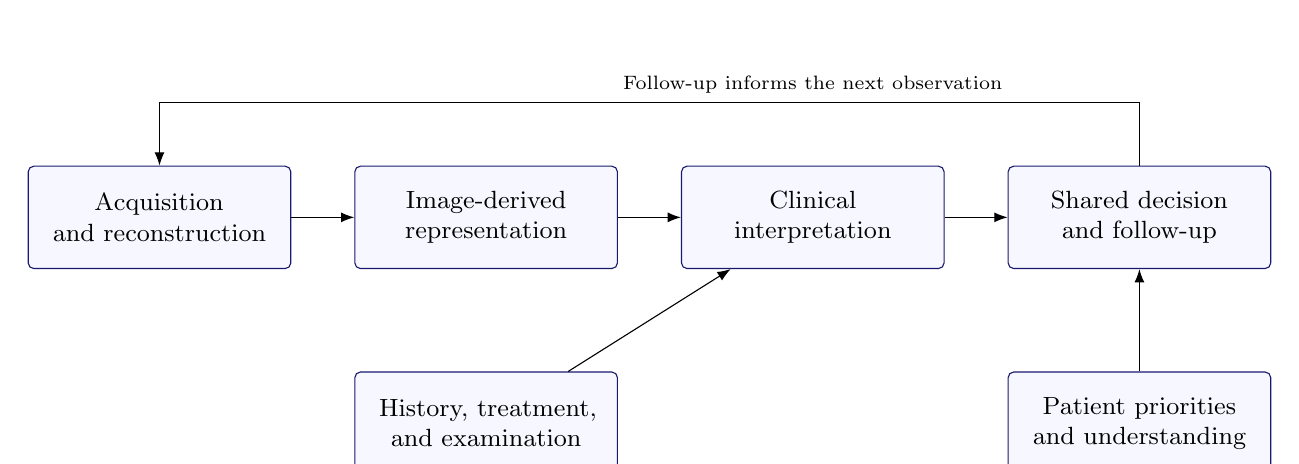
\begin{tikzpicture}[node distance=9mm and 8mm,>=Latex, every node/.style={font=\small},box/.style={draw=MidnightBlue,rounded corners=2pt,align=center,text width=31mm,minimum height=13mm,fill=blue!3}]
\node[box] (acq) {Acquisition\\and reconstruction};
\node[box,right=of acq] (img) {Image-derived\\representation};
\node[box,right=of img] (review) {Clinical\\interpretation};
\node[box,right=of review] (act) {Shared decision\\and follow-up};
\node[box,below=13mm of img] (context) {History, treatment,\\and examination};
\node[box,below=13mm of act] (patient) {Patient priorities\\and understanding};
\draw[->] (acq)--(img);\draw[->] (img)--(review);\draw[->] (review)--(act);
\draw[->] (context)--(review);\draw[->] (patient)--(act);
\draw[->] (act.north) -- ++(0,8mm) -| (acq.north);
\node[above=8mm of review,font=\scriptsize] {Follow-up informs the next observation};
\end{tikzpicture}
\caption{An original conceptual diagram of clinical interpretation. Arrows denote information or feedback, not validated causal effects. A model's output becomes useful within a larger process. The illustration synthesizes the imaging perspective of \citet{lundervold2019} and the clinical evaluation emphasis of \citet{decide2022}.}
\label{fig:pathway}
\end{figure}

\subsection{A published glioma example: from compartments to regional burden}
\citet{lundervold2026glioma} provide a concrete research counterpart to the hypothetical vignette. Their feasibility pipeline uses several complementary MRI contrasts: T1, gadolinium-enhanced T1, T2, and fluid-attenuated inversion recovery (FLAIR). T1 and T2 denote contrasts based on different tissue relaxation properties; FLAIR suppresses cerebrospinal-fluid signal. The pipeline combines these images with deep-learning tumour segmentation and subject-specific anatomical parcellation (division into named brain regions). It relates central non-enhancing/necrotic tumour, enhancing tumour, and surrounding oedema to brain regions, producing volumes and regional tumour-burden ``hit-plots''. Evaluation included 50 UCSF-PDGM glioblastoma cases and one longitudinal LUMIERE case with six timepoints. The reported agreement supports the evaluated segmentation task; the regional profiles supply anatomical context, while their effect on treatment decisions and outcomes remains to be established.

This example makes the distinction between representation and interpretation tangible: a tumour mask describes spatial membership, a volume summarizes extent, and a regional-burden profile describes overlap with named anatomy. Each summary preserves a different aspect of the image. Ask which aspect supports the intended clinical conclusion, and which evidence about tissue viability or function would have to come from another measurement.

Figures~\ref{fig:glioma-source-A3} and~\ref{fig:glioma-source-6} reproduce source Figure A3 and Figure 6, respectively. The original legends retain source numbering; [60] denotes \citet{suter2022}. Detailed descriptions are added here.

\clearpage
\begin{figure}[!ht]
\centering
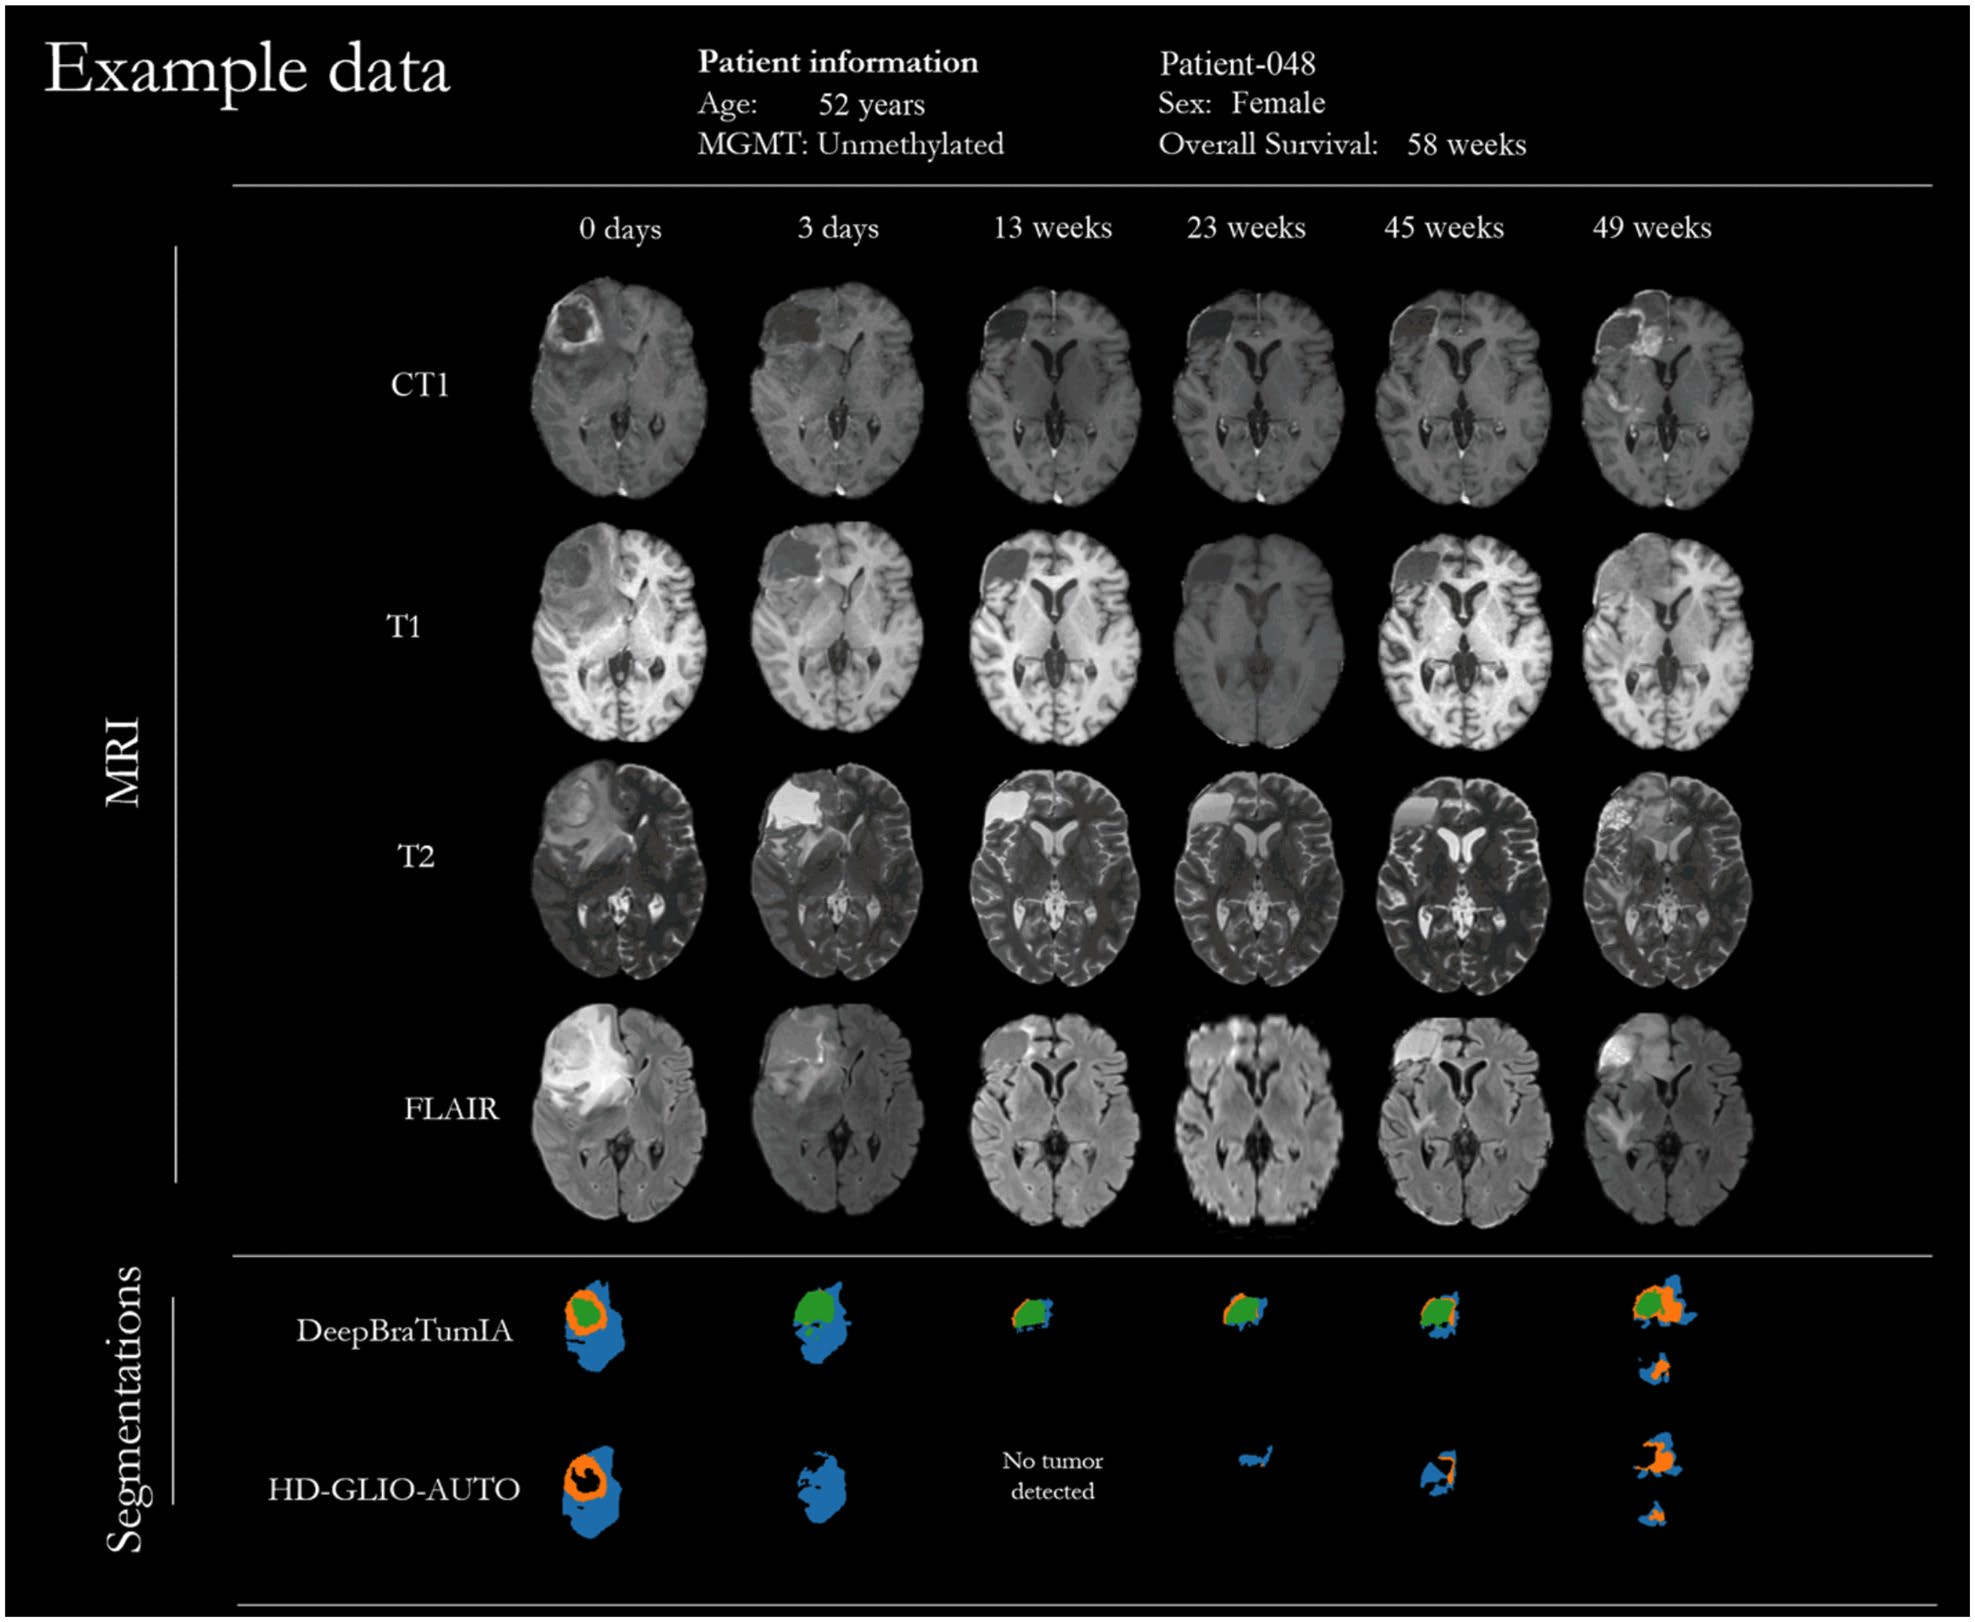
\includegraphics[width=0.90\linewidth]{figures/lundervold2026-appendix-A3.jpeg}
\caption[Longitudinal mpMRI and comparator segmentations: source Figure A3]{\textbf{Reproduction of Appendix Figure A3 from \citet{lundervold2026glioma}. Original legend:} ``Example of longitudinal data on GBM from the LUMIERE collection. CT1/T1: Post-/pre-contrast T1-weighted, T2-weighted, and fluid-attenuated inversion recovery (FLAIR). For this individual, the entire contrast enhancement was fully removed. Following a phase of complete response, there was a progression characterised by a highly rapid growth rate. In the present study we process all six mpMRI examinations of Patient-048 under the unified evaluation framework (Results, Figure 6). From Suter et al. [60] \url{https://www.nature.com/articles/s41597-022-01881-7} (CC BY 4.0).''}
\label{fig:glioma-source-A3}
\end{figure}

{\small\textbf{Detailed description.} Six columns follow the same published LUMIERE case from baseline and day 3 to weeks 13, 23, 45, and 49. Four axial MRI rows display contrast-enhanced T1 (CT1), unenhanced T1, T2, and FLAIR. The baseline images show a conspicuous lesion with enhancement and surrounding signal abnormality; the immediate postoperative images show the altered tumour bed. The later columns allow visual comparison of the low-enhancement interval and subsequent recurrence. Two lower rows show the corresponding colour-coded DeepBraTumIA and HD-GLIO-AUTO segmentation outputs. These are comparator outputs from the LUMIERE illustration, not the unified SegResNet output plotted next. Their colours should not be transferred to the next graph's legend. The ``No tumor detected'' annotation is an output of the displayed segmentation method, not proof of absence of all tumour cells. A single axial view illustrates morphology, while volumetry uses the three-dimensional masks. The source legend's description of complete removal should likewise be distinguished from the small postoperative enhancing volume estimated by the unified model.}

\medskip
{\footnotesize\textbf{Attribution.} Image extracted unchanged from Appendix Figure A3, printed p.~28 (PDF p.~29), of \citet{lundervold2026glioma}; the source credits \citet{suter2022}. Both articles identify CC BY 4.0 licensing. Image resized only; original legend retained, with typography reset. Licence: \url{https://creativecommons.org/licenses/by/4.0/}.}

\clearpage
\begin{figure}[!ht]
\centering
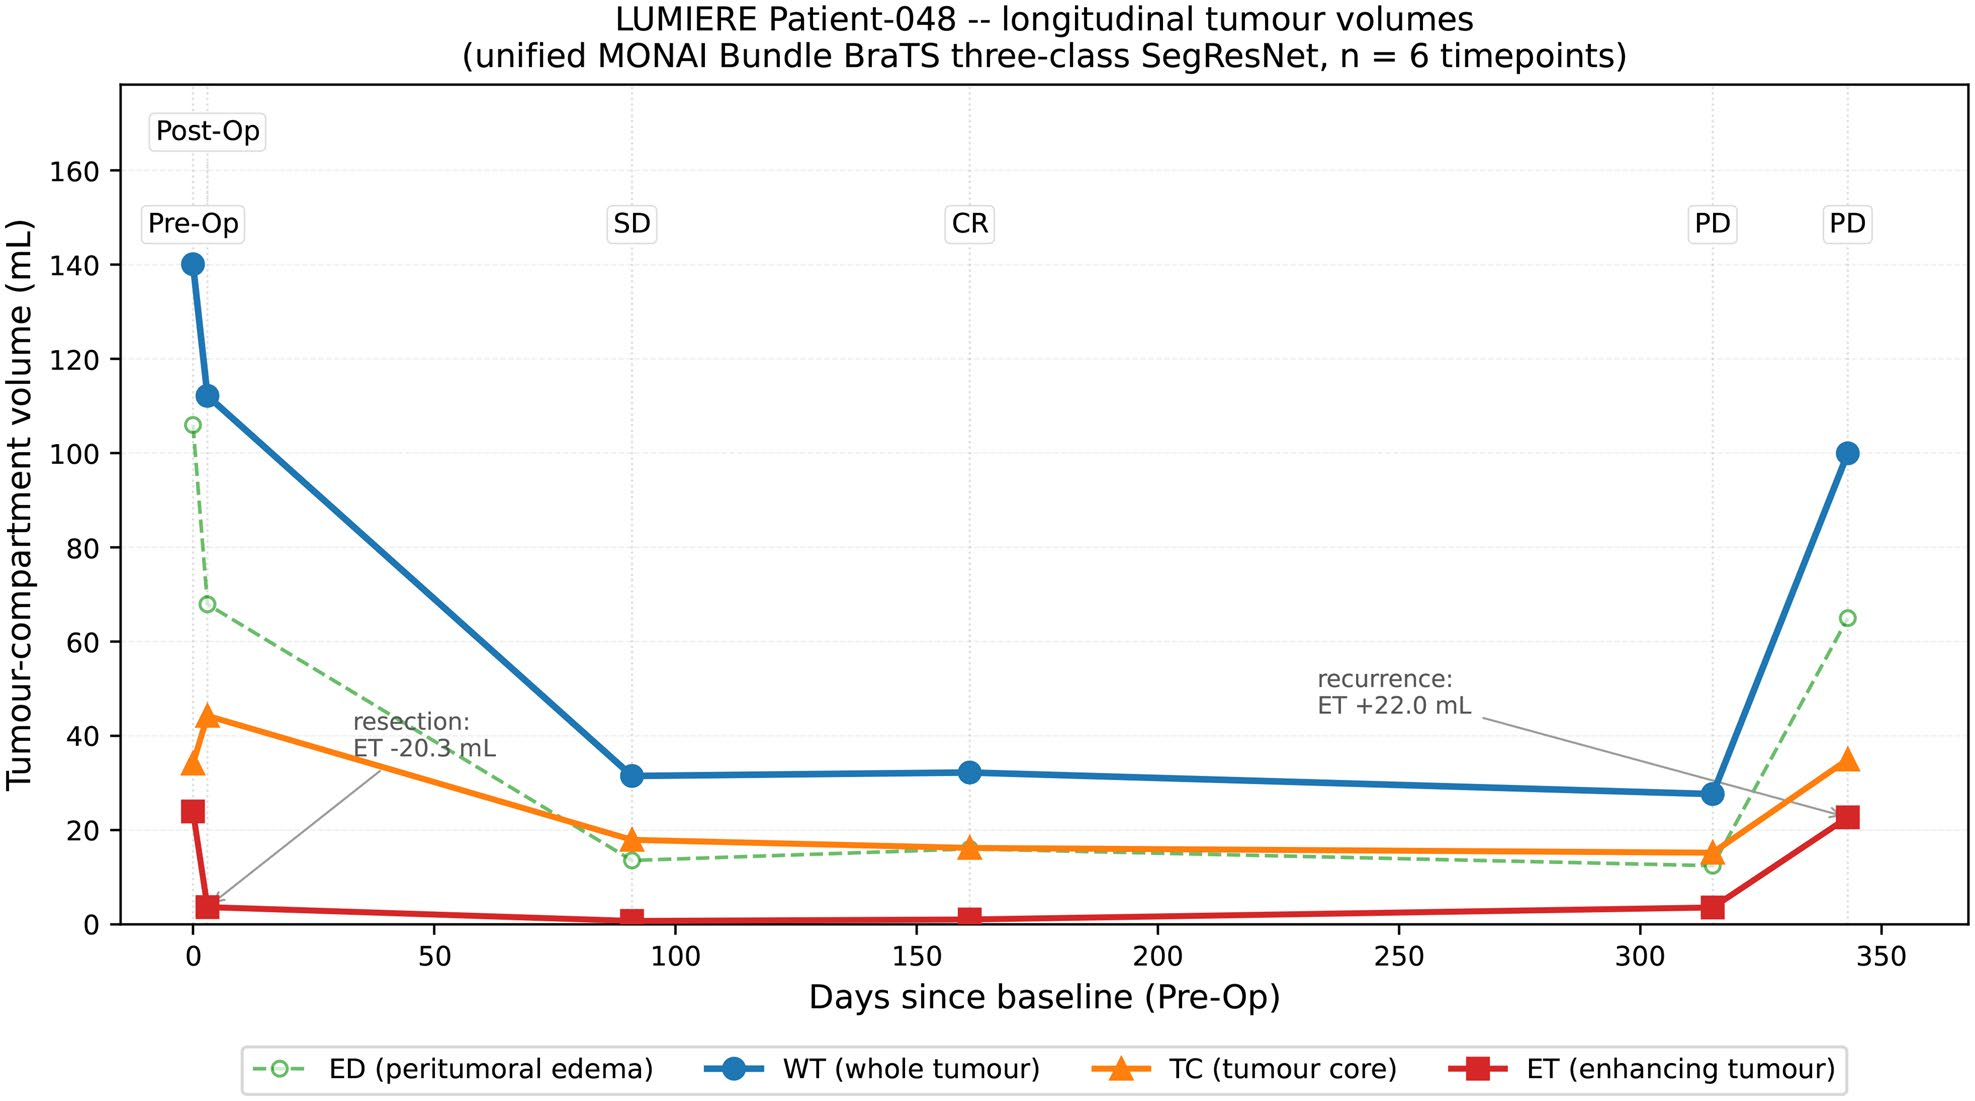
\includegraphics[width=\linewidth]{figures/lundervold2026-figure-6.jpeg}
\caption[Longitudinal SegResNet volumes: source Figure 6]{\textbf{Reproduction of Figure 6 from \citet{lundervold2026glioma}. Original legend:} ``LUMIERE Patient-048 -- longitudinal tumour volumes from the unified MONAI Bundle BraTS three-compartment SegResNet ($n=6$ timepoints). Per-compartment volume (mL) on a continuous day-resolved time axis: enhancing tumour (ET, red), necrotic core (NCR, blue), tumour core (TC$=$NCR$+$ET, dashed), edoema (ED, green), and whole tumour (WT$=$NCR$+$ED$+$ET, black). RANO labels (Pre-Op, Post-Op, SD, CR, PD, PD) and selected clinical event annotations (post-operative ET drop; recurrence trough/peak) are shown above the trajectories. LUMIERE anonymisation disclosure: the two baseline scans (week-000-1, week-000-2) carry day-resolution from the LUMIERE archive (0 and 3 days, respectively); from week-013 onward LUMIERE reports timepoints as floor-weeks [60], so days for week-013 / -023 / -045 / -049 are computed as week$\times7$ and carry a $\pm3$ day uncertainty.''}
\label{fig:glioma-source-6}
\end{figure}

{\small\textbf{Verification note.} The published legend above does not match all plotted encodings. The image actually shows \emph{four} series: WT as solid blue circles, TC as solid orange triangles, ET as solid red squares, and ED as dashed green open circles. NCR is not plotted separately. The image and original legend have been retained without correction; the description below follows the displayed plot.}

\medskip
{\small\textbf{Detailed description.} The horizontal axis gives days since baseline; the vertical axis gives compartment volumes in millilitres. Six visits correspond to days 0, 3, 91, 161, 315, and 343, with the source's timing qualification retained above. WT falls markedly after the preoperative scan, remains much lower through the middle visits, then rises at the final visit. ET also drops sharply after surgery, stays near the volume floor, and increases again at recurrence. The source text reports WT/ET of 140.1/24.0 mL at baseline, postoperative ET of 3.7 mL, and final WT/ET of 100.0/22.7 mL. The displayed RANO labels identify stable disease (SD), complete response (CR), and progressive disease (PD), in addition to the surgical visits. These clinical categories are annotations, not classifications established by a volume curve alone. Lines connect discrete examinations; they are not continuous observations of tumour growth. TC and WT are composite volumes, so the four plotted quantities should not be summed.}

\medskip
{\footnotesize\textbf{Attribution.} Image extracted unchanged from Figure 6, printed p.~15 (PDF p.~16), of \citet{lundervold2026glioma}, \copyright~2026 The Author(s), published by Informa UK Limited, trading as Taylor \& Francis Group. CC BY 4.0: \url{https://creativecommons.org/licenses/by/4.0/}. Image resized only; original legend retained, with typography reset.}
\clearpage


A useful exercise (a thought experiment) is to ask three people to state the output they need. The imaging scientist might require a reproducible boundary estimate. The clinician might require evidence that a change alters management. The patient might require an explanation of what remains uncertain and what happens next. These are compatible purposes, but they demand different evaluation targets. Confusing them makes technical improvements look more clinically complete than they are.

\learningcheck{A measured volume change needs separate evidence about measurement reliability, biological interpretation and consequences for a decision.}{A volume increases from 10 to 12~mL: what would you need to determine whether the change reflects progression?}

\section{AI-assisted model development and numerical verification}\label{sec:growth}
Marr's questions help organize an AI-assisted simulation. The \emph{task} is to investigate how cell spread and proliferation change a density field. The \emph{representation} is density over space and time; the algorithm approximates the field's evolution. The \emph{implementation} chooses a spatial grid, time steps, boundary treatment and numerical precision. Checking an implementation is distinct from testing whether the represented biology is adequate.

\subsection{Read the growth equation}
A population Fisher--Kolmogorov--Petrovsky--Piskunov (Fisher--KPP) model describes cell density $c(\mathbf{x},t)$ at position $\mathbf{x}$ and time $t$ by
\begin{equation}
\partial_t c=\nabla\!\cdot(D\nabla c)+\rho c(1-c/K),
\qquad \mathbf{n}\!\cdot D\nabla c=0\quad\text{on the boundary}.
\end{equation}
Read the equation as \emph{change in density = redistribution through space + local growth}. Its quantities and operators have distinct roles:
\begin{itemize}
\item $\partial_t c$ is the rate of change at a fixed location. The symbol $\partial$ denotes a derivative with respect to one variable while the others are held fixed.
\item $\nabla c$ is the spatial gradient: it records how density varies with position. The transport flux is $-D\nabla c$, toward lower density in isotropic diffusion. The divergence $\nabla\!\cdot(D\nabla c)$ gives the resulting local net gain or loss through transport.
\item $D$, in mm$^2$/day, controls dispersal; it may be a scalar coefficient or a tensor describing directional differences. The proliferation rate $\rho$ is in day$^{-1}$. Both $c$ and the carrying capacity $K$ are in cells/mm$^3$.
\item The growth term is approximately $\rho c$ when $c$ is small compared with $K$, and becomes zero at $c=K$. The outward unit normal $\mathbf{n}$ specifies the direction perpendicular to the boundary. The boundary equation sets transport through that surface to zero.
\end{itemize}
The no-flux boundary specifies a closed transport domain; growth inside it can still change the total cell number. The migration/proliferation dichotomy known as \emph{go-or-grow} is a separate mechanistic hypothesis \citep{hatzikirou2012}; the displayed equation has no explicit switching between migratory and proliferative cell states.

\begin{perspectives}{growth modelling}
\textbf{Biomedical and imaging perspective.} Read $c$ as an assigned cell density and ask how a measurement would relate to it. In the threshold example below, first change only the display threshold at a fixed time, then change a growth parameter while keeping the threshold fixed. Which change alters the simulated state, and which changes only its displayed extent?

\textbf{Computational perspective.} Separate the evolution equation from the rule that converts its field into observations. Use Notebook 13 to check growth, transport and boundaries independently; use 14a--14c to investigate thresholding, anatomy and fitting. Track which assumptions are shared by the observation generator and fitted model before interpreting a withheld forecast.
\end{perspectives}

\subsection{Check the implementation using simpler cases}
An AI assistant can propose equations, implement a solver and construct a display. To check the solver, remove transport by setting $D=0$. At each location the equation becomes $dc/dt=\rho c(1-c/K)$. For a starting density $c_0>0$ and constant $\rho,K$, its exact solution is
\[
c(t)=\frac{K}{1+(K/c_0-1)e^{-\rho t}}.
\]
At $t=0$ the denominator is $K/c_0$, giving $c(0)=c_0$; for $\rho>0$, the solution approaches $K$ as time increases. Comparing the numerical trajectory with this formula tests the implemented growth term.

Next set $\rho=0$ and retain zero boundary flux. Transport should redistribute cells while conserving their total number. A second check is needed for their location: periodic wraparound can conserve the total while moving cells across the wrong boundary. Reducing grid spacing and time steps tests how discretization error changes with resolution. \coursenotebook{13_verified_growth_model.ipynb}{Notebook 13} implements a small independent one-dimensional reference, plus a uniform-compartment coupled limit. An optional check exercises the pinned three-dimensional implementation on synthetic arrays without reading anatomy or patient data.

The separate BrainWeb demonstration adds an illustrative coupling of viable cells, oxygen and necrotic material, and compares it with a matched Fisher--KPP reference. Its reduced closure (the chosen relationships connecting the variables) and parameters are hypotheses for exploration. Removing oxygen uptake should recover the specified baseline; this checks consistency of the coupled equations. Testing physiological adequacy additionally requires independent oxygen and cell-density measurements, parameter estimation and withheld outcomes. The following exercises examine the simpler Fisher--KPP model on anatomy and with generated observations; they do not reproduce the full coupled implementation. The slide-to-resource guide records the external implementations and their versions.

\subsection{Separate a density field from a displayed boundary}
% Generated by scripts/build_growth_lessons.py; do not edit numbers by hand.
\newcommand{\GrowthBurden}{20.60}
\newcommand{\GrowthVolumeLow}{93.12}
\newcommand{\GrowthVolumeHigh}{36.67}
\newcommand{\GrowthForecastError}{0.00465}
\newcommand{\GrowthPersistenceError}{0.06288}

\coursenotebook{14a_growth_density_and_thresholds.ipynb}{Notebook 14a} extends verification into interpretation. It adapts the tissue and threshold experiments of the companion glioma teaching material \citep{gliomateaching2026}. For a spatially constant carrying capacity, define the dimensionless fraction $u=c/K$. The equation becomes $\partial_t u=\nabla\!\cdot(D\nabla u)+\rho u(1-u)$. An invented two-dimensional tissue map supplies a controlled comparison before introducing an anatomical phantom. Spatially varying cell motility in grey and white matter has a published glioma-model precedent \citep{swanson2000}; the coefficients here are assigned teaching values, not estimates from that study or a particular MRI.

For pixel area $a$, two readings of the same field are
\[
B_{2D}=a\sum_i u_i,\qquad A_\tau=a\sum_i\mathbf{1}[u_i\geq\tau].
\]
The indicator $\mathbf{1}[\cdot]$ is one when the condition holds and zero otherwise. The integral $B_{2D}$ weights every pixel by its density fraction; $A_\tau$ counts selected pixels equally. Both have units mm$^2$, but neither is a cell count or whole-tumour volume. A 1~mm$^2$ pixel at $u=0.8$ contributes 0.8~mm$^2$ to the integral and 1~mm$^2$ to $A_{0.2}$. Raising the reading threshold changes the displayed boundary without changing the simulated state.

\begin{figure}[!ht]\centering
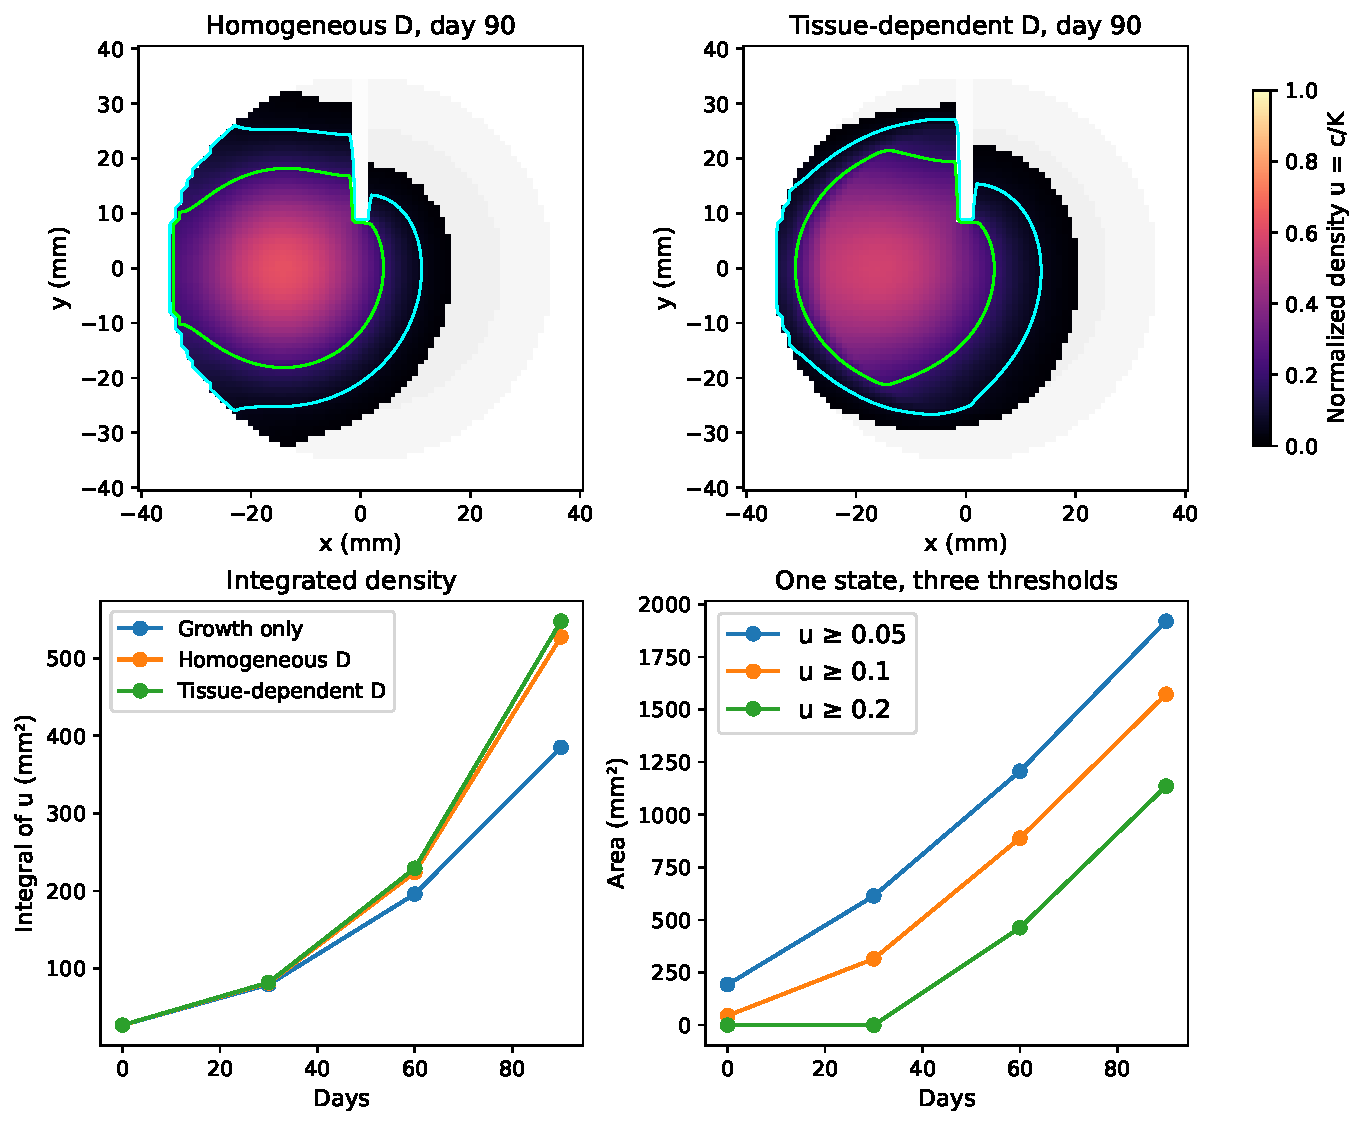
\includegraphics[width=.92\linewidth]{figures/growth_tissue_thresholds.pdf}
\caption{A constructed two-dimensional domain, not a patient image or BrainWeb slice. Homogeneous and tissue-dependent scalar diffusivities have the same domain mean, with the initial state and proliferation rate fixed. They need not produce the same spatial field or integrated density. The lower-right panel changes only the threshold applied to one simulation. The coefficients, closed barriers and thresholds are teaching assumptions.}\label{fig:growth-thresholds}
\end{figure}
\FloatBarrier

\subsection{Use anatomy without mistaking it for a tumour observation}
\coursenotebook{14b_brainweb_growth.ipynb}{Notebook 14b} uses the original normal BrainWeb digital phantom and its tissue labels \citep{collins1998,cocosco1997}. Both input volumes are bundled with the teaching code; no companion checkout or separate data download is needed. Its simulated T1 contains no tumour. The density seed and growth rates are specified separately. The loader checks paired image geometry and file checksums, then samples every fourth native voxel at 4~mm spacing while retaining physical coordinates. This coarse representation can lose thin barriers; changing the sampling changes both the numerical grid and tissue geometry.

The growth domain contains grey matter, white matter and the phantom's glial class, which shares the grey-matter coefficient. CSF and other classes are excluded and act as no-flux barriers. We assign $D_{WM}=0.5$ and $D_{GM}=0.1$~mm$^2$/day and $\rho=0.04$~day$^{-1}$. A Gaussian seed with standard deviation 8~mm and peak $u=0.12$ is centred at RAS+ coordinates $(-24,-12,24)$~mm and masked to that domain. RAS+ denotes axes increasing rightward, anteriorly and superiorly. A homogeneous comparison uses the mean coefficient over the same domain. These are spatially heterogeneous \emph{scalar} coefficients, not fibre-directed diffusion tensors.

For voxel volume $v$ in mm$^3$, normalized burden is $B=v\sum_i u_i/1000$ in mL, while threshold volume is $V_\tau=v\sum_i\mathbf{1}[u_i\geq\tau]/1000$. At 4~mm spacing, one voxel is 0.064~mL: at $u=0.25$ it contributes 0.016~mL to $B$ and 0.064~mL to $V_{0.2}$. In the specified tissue-dependent day-90 run, $B=\GrowthBurden$~mL, whereas $V_{0.05}=\GrowthVolumeLow$~mL and $V_{0.2}=\GrowthVolumeHigh$~mL. These computed quantities are not observed lesion volumes. An absolute model-implied cell count would additionally require a justified $K$ in cells/mm$^3$; a comparison with MRI would require a measurement model for the relevant sequence.

\begin{figure}[!ht]\centering
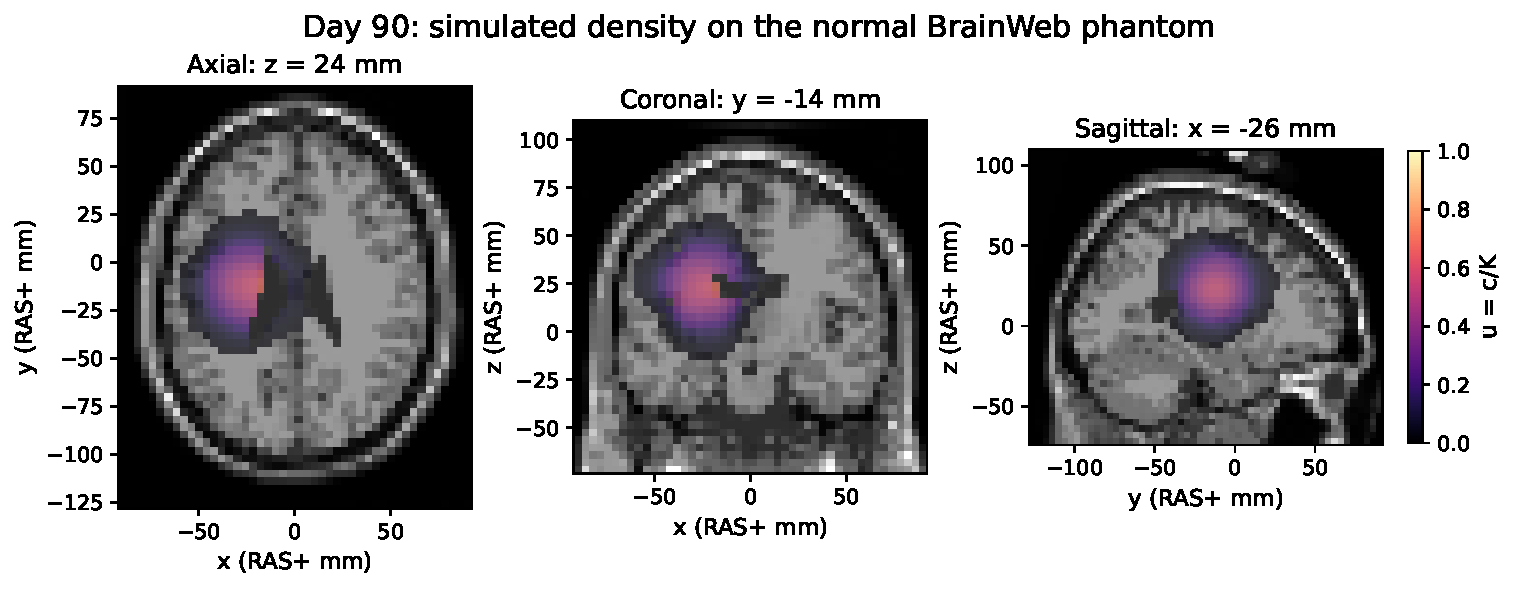
\includegraphics[width=\linewidth]{figures/growth_brainweb.pdf}
\caption{Simulated normalized density at day 90 on the normal BrainWeb phantom. Orthogonal planes pass through the specified seed, with actual sampled RAS+ coordinates labelled. The colour scale is fixed from zero to one; density below 0.01 is hidden for display and overlay opacity is 0.8. Geometry supplies anatomical context; the tumour field and rates are assigned. BrainWeb attribution: \citet{collins1998,cocosco1997}.}\label{fig:growth-brainweb}
\end{figure}
\FloatBarrier

\subsection{Estimate parameters, then test a withheld forecast}
A forward model computes a state from chosen parameters; an inverse problem estimates parameters from observations. \coursenotebook{14c_growth_parameter_recovery.ipynb}{Notebook 14c} makes this distinction testable with generated observations on BrainWeb anatomy. The unknowns are a multiplier $s$ of both tissue diffusivities and a shared proliferation rate $\rho$. The white-to-grey ratio remains fixed at five. The generator uses the stated seed, $s=1$ and $\rho=0.04$~day$^{-1}$ on a 6~mm grid. Seed, tissue geometry, carrying-capacity normalization and ratio are known assumptions.

Define an observation operator $\mathcal B$ that averages each non-overlapping $2\times2\times2$ block into a 12~mm sample. Unmatched high-index edge cells are trimmed consistently. Independent Gaussian noise with standard deviation 0.005 in normalized-density units is added without clipping. Thus
\[
y_i=\mathcal B[u(t_i;s,\rho)]+\epsilon_i.
\]
This is a density-proxy measurement model, not an MRI simulator. A 72~mm cube around the seed is specified before noise generation and fitting. Least squares within that cube compares 63 candidate pairs using days 20, 40 and 60 only. Day 90 is withheld from parameter selection. The generator uses 0.5-day time steps and candidates use 1-day steps, but both share the spatial grid, equation and observation operator.

For noise seed 7, the grid search selects the generating pair, which is present among the candidates. At day 90 the RMSE (root mean squared error) against the withheld noisy spatial samples is \GrowthForecastError, compared with \GrowthPersistenceError\ for persistence, which simply carries the observed day-60 map forward. These are normalized-density units, not MRI intensity or clinical error scores. The search-grid minimum is not a confidence interval, and one favourable noise realization does not establish robustness or interval coverage. Unknown initialization, separate tissue rates and an imperfect observation operator would create additional inference questions. The source companion contains more extensive recovery and uncertainty experiments; those results are not claimed by this compact exercise.

\begin{figure}[!ht]\centering
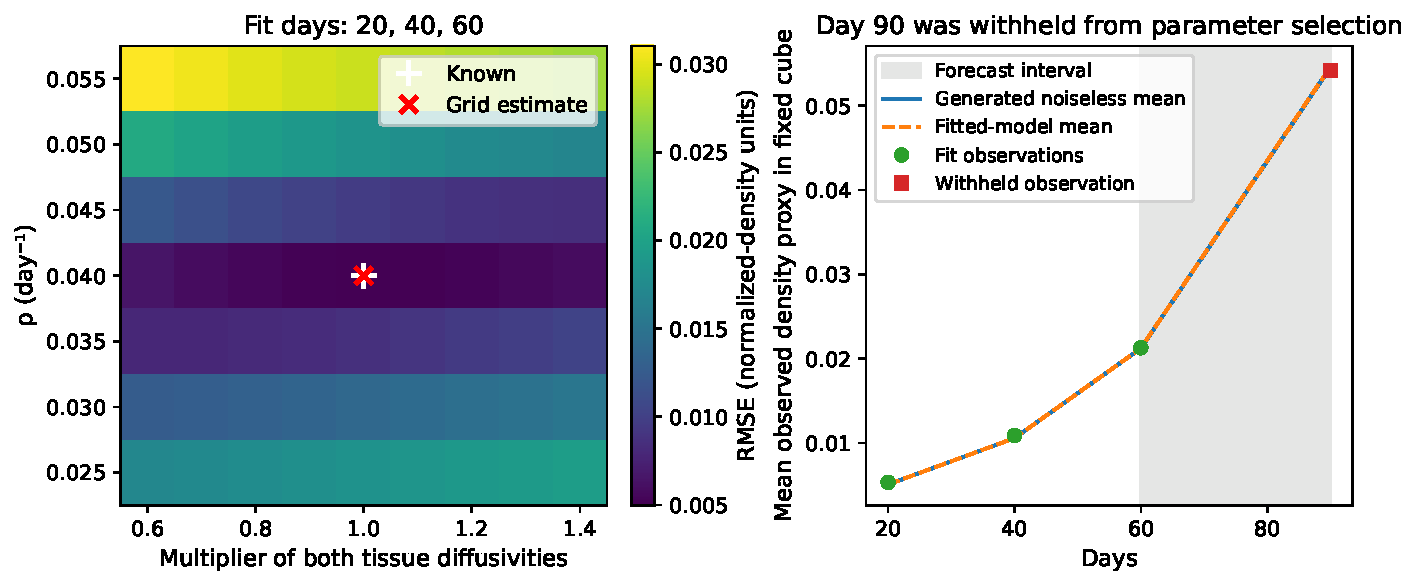
\includegraphics[width=\linewidth]{figures/growth_recovery.pdf}
\caption{Generated-data recovery and a withheld forecast on the 6~mm BrainWeb grid. The left panel shows fitting error over the candidate grid. The right panel averages samples within the fixed observation cube for display; fitting and reported RMSE use the spatial samples individually. Day 90 does not enter fitting. Shared model and measurement assumptions make this a controlled inference exercise, not independent biological validation.}\label{fig:growth-recovery}
\end{figure}
\FloatBarrier

\paragraph{Interactive exploration.} Notebooks 14a--14c provide live controls for tissue rates, numerical settings and inference choices. Time, threshold and image-view controls in 14a/14b read cached states; changing simulation parameters requires a new run. Notebook 14c varies noise, early observation times and search resolution while keeping day 90 withheld. The paper's figures retain the fixed reference settings stated above.

This example gives domain expertise a concrete role in AI-assisted research: specify the scientific question, check units and assumptions, compare with independent solutions, inspect failures, and distinguish an implemented proposal from an empirically supported model.

\learningcheck{A limiting case can check a solver against an independent answer; biological adequacy needs measurements of the system being modeled.}{A diffusion solver conserves total cells but wraps transport around the boundary: which additional test would reveal the error?}

\section{Shared vocabulary needs operational definitions}\label{sec:vocabulary}
\subsection{Representation: similar geometry is informative, but incomplete}
A representation makes some distinctions available to a downstream process: a later computation that uses it. For a model, this can mean that a layer's activations support a classifier or predict neural responses on held-out stimuli. For a person, representations are inferred from behavior, physiology, and interventions. Their relationships to meaning, action, and experience require additional arguments. ``Representation'' is useful precisely because it is broad, but that breadth can conceal changes in the claim being made.

For a concrete model example, freeze an image encoder (keep fixed the weights that map an image to a feature vector) and fit a linear classifier to its embeddings to distinguish lesion-containing from lesion-free patches. Evaluate it on patients excluded from both encoder training and classifier fitting. Successful decoding indicates that this distinction is available to that readout under those conditions. It does not show that the encoder's original output head uses it, or that the signal is the lesion rather than a correlated feature.

For a human comparison, ask participants to categorize objects viewed from unfamiliar angles and test whether an independently fitted encoding model predicts their measured visual responses. Behaviour, neural prediction, and a causal intervention address different claims. Recognizing a cup across views, reaching to grasp it, and experiencing its appearance are related phenomena, but a decoder of object category measures only one part of that relationship. An intervention that disrupts grasp selection would add evidence about action; category decoding alone would not establish the experience of seeing.

\citet{yamins2014} tested a more specific connection. They optimized hierarchical models for object categorization and assessed their ability to predict neural responses to images in macaque visual cortex. The stimuli varied object appearance and included background variation. Higher model representations predicted inferior temporal responses, while intermediate representations predicted V4 responses. The important point is that an engineering objective helped select representations informative about independently measured biology; a network was not simply assigned a cortical label because its diagram looked hierarchical. This is a substantive bridge between engineering and neuroscience. Its evidential force depends on the stimuli, recording conditions, model comparisons, and evaluation procedure. Predicting some neural responses does not identify the biological learning rule. It also does not show that every layer has a one-to-one cortical counterpart. A model may approximate an input-output relation while implementing it differently.

An optimization-based approach to neuroscience asks how objective functions, learning rules, and architectures jointly constrain behavior \citep{richards2019}. For medical AI, this motivates comparing models under changed conditions rather than only comparing average test scores. Does a representation retain the lesion information needed after an acquisition change? Does it support appropriate abstention---declining to provide an ordinary prediction---when a required sequence is absent? These questions connect representation to its practical role without assuming that a successful embedding explains the whole person.

An illustrative experiment makes the optimization argument tangible. Train the same architecture with either a lesion-label objective or an image-reconstruction objective; separately hold the objective fixed while changing the architecture or learning rule. Use matched data and report any unmatched training budget. Then test whether lesion information remains decodable and usable after a controlled change in image contrast. The first comparison examines the effect of the objective; the others examine architectural and learning constraints. This is a proposed experiment, not a result attributed to \citet{richards2019}.

In the MRI vignette, compare lesion masks on paired images with identical anatomy but a specified synthetic intensity transformation, and then validate on an independent acquisition setting. Report lesion-wise failures and boundary changes as well as average overlap. Separately remove a required sequence and record whether a system designed to abstain does so. Preserved average performance, preserved lesion information, and appropriate abstention are three distinct outcomes. Synthetic transformations help isolate a question, but do not reproduce every consequence of a scanner change.

\learningcheck{Information decodable from a representation is available to the chosen readout; an intervention tests whether a particular output uses it.}{A lesion label is decodable from an embedding: what intervention would test whether the original classifier depends on lesion information?}

\subsection{Attention: a weighting operation and a family of human capacities}
A Transformer is a neural-network architecture that updates representations using attention and other operations. Its attention operation lets one input position combine information from other positions using weights that depend on their representations. The positions can contain image patches or tokens: units such as words, word parts or characters. A query specifies what is being matched, keys provide the quantities against which it is matched, and values carry the information to be combined. For example, an image-patch representation can be updated using information from other patches. These are learned numerical transformations, rather than literal questions or labels supplied by a person. Appendix~\ref{app:attention} gives the equation, dimensions, and a worked calculation \citep{vaswani2017}.

This computational definition does not define human attention, which is studied through selective processing, task performance, and neural mechanisms. The shared name invites hypotheses about selection; it does not establish identity. A useful teaching question is: what information is being selected, by which operation, and for which output?

A heatmap is a display format, not a single explanation method. An attention map displays internal weighting coefficients. A gradient saliency map displays derivatives: how a chosen output changes under sufficiently small input changes. A perturbation map compares outputs after specified input changes. These quantities answer different questions; none becomes a clinical explanation simply by being overlaid on an anatomical image.

To see the distinction, imagine a classifier whose overlay highlights an enhancing region. This may be compatible with appropriate use of lesion information, but visual plausibility alone cannot exclude dependence on another feature. A saliency method can even produce plausible structure after learned parameters have been randomized. Model-parameter and training-label randomization are therefore useful sanity checks: an explanation that claims to describe a learned decision should be examined for dependence on that learning \citep{adebayo2018}. Passing these checks is a starting point, not proof of a biological mechanism.

A complementary exercise is to change a suspected acquisition cue while preserving the lesion as far as possible, then inspect the prediction and explanation together. Such experiments also need controls: masking a region can create an unfamiliar image, so a changed prediction may reflect the intervention artifact. The explanatory claim and the validity of its test both require scrutiny. When an interpretable model can meet the clinical task, the trade-off should be examined explicitly \citep{rudin2019}.

For a specific controlled example, put a bright site marker outside the anatomy in otherwise identical synthetic images. Change only that marker and recompute the score and maps. The anatomy is exactly preserved by construction, so a score change establishes sensitivity to the marker in this model. In a real exported image, remove or replace an existing border annotation without altering anatomical pixels, and compare with an equally sized control edit elsewhere in the border. The latter comparison helps detect sensitivity to the editing procedure. It still cannot establish that the marker explains all errors or that arbitrary inpainting is a valid counterfactual.

Appendix~\ref{app:maps} and \texttt{code/src/brainsmodels/attention\_maps.py} make these distinctions executable. A small, explicitly specified self-attention sublayer and scalar readout produce an attention matrix, a signed input gradient, and a patch-occlusion map for the same synthetic input (\coursenotebook{08_attention_maps.ipynb}{notebook 08}; the two-key calculation is in \coursenotebook{10_two_key_attention.ipynb}{notebook 10}). The example also changes a marker while holding the central pattern fixed and randomizes parameters. It is a transparent computational exercise, not a trained clinical Transformer or a reproduction of a saliency validation study.

\begin{perspectives}{attention and image overlays}
\textbf{Biomedical and imaging perspective.} Before interpreting an overlay, identify what its colours encode and which output is being examined. In the synthetic marker experiment, compare the score before and after the marker changes while the central pattern stays fixed. Anatomical plausibility and dependence of a prediction on a feature are separate questions.

\textbf{Computational perspective.} Work through Appendix~\ref{app:attention} with Notebook 10: keep query and keys fixed, then change the second value from 10 to $-10$. Explain why the weights stay fixed while the output changes. In Notebook 08, compare a local derivative with a finite replacement, keeping the output target and replacement baseline explicit.
\end{perspectives}

\learningcheck{Attention weights, gradients and finite replacements describe different operations and must be interpreted with their output and scale.}{If attention weights stay fixed while the values change, must the final weighted output stay fixed?}

\subsection{Memory: distinguish parameters, context, retrieval, and recollection}
A language model estimates probabilities for tokens given a preceding context. In a deployed language-model system, ``memory'' can refer to trained parameters, the current context (input available for the current calculation), an external retrieval store, or an application-maintained record. These differ in persistence, update mechanism, provenance, and access. A statement available through retrieval may disappear when the index changes; a statement encoded in parameters may be difficult to locate or revise. Neither should be casually equated with an autobiographical episode.

For example, trained parameters may support completing a familiar phrase; a current prompt may contain a newly supplied fictional identifier; retrieval may supply a versioned teaching protocol; and an application may reload the preference ``explain abbreviations.'' Only the last three examples require access to those particular records at inference time. Even there, the mechanisms can overlap: a retrieved passage usually becomes part of the generator's context.

Autobiographical remembering adds a different explanatory target. Remembering one's first day in a laboratory can include a place, an event sequence, personal significance, and a sense of having been there. A system could store and accurately reproduce a dated account of that day, but this establishes access to information about an event, not the first-person experience of recollecting it. The distinction does not prove that artificial recollection is impossible; it specifies why factual accuracy alone cannot settle the question.

Consider a report assistant that correctly recalls a patient's stated preference within a conversation. The preference may be present in the current input, loaded from an application record, or retrieved from a document. Correct output alone does not reveal which mechanism supplied it. Removing the earlier message, disabling retrieval, or changing the stored record are different interventions. They help identify the source of the behavior without assuming that the system has recollected an event.

\begin{table}[htbp]\centering\small
\caption{Four engineering uses of ``memory.'' Persistence depends on the deployed system; these are mechanisms, not human memory categories.}
\begin{tabularx}{\linewidth}{p{24mm}XX}\toprule
Mechanism & Concrete illustrative example & A discriminating check \\\midrule
Parameters & A familiar phrase can be completed without providing its source in the prompt; learned weights influence the completion. & Compare documented model versions or controlled training interventions.\\
Context & A prompt states that fictional sample Q7 has label blue; the next answer uses that statement. & Remove the relevant passage while holding the other input fixed.\\
Retrieval & A versioned teaching protocol is retrieved from an index and supplied with the question. & Inspect retrieved sources and repeat with retrieval disabled.\\
Application record & Software reloads the saved preference ``explain abbreviations'' at the start of a new session. & Inspect what was saved and what is actually reintroduced.\\\bottomrule
\end{tabularx}
\end{table}

Retrieval-augmented generation explicitly combines parametric and external information \citep{lewis2020}. Access to a source does not guarantee that the source was selected correctly or used faithfully. In a clinical report exercise, one should therefore record both the retrieved passage and the generated statement. Provenance is a property to inspect, rather than infer from the confidence of the language.

In complementary learning systems theory, rapid hippocampal learning and slower neocortical learning help reconcile two needs: acquiring a particular event and integrating regularities across events without excessive interference \citep{mcclelland1995}. A teaching example is learning a new colleague's name after one introduction while gradually learning the conventions of a new laboratory. These are illustrative cases, not clean anatomical assignments: the theory concerns interacting systems, and learning rate alone does not identify a brain region.

An engineering comparison could store each new meeting note immediately in an external index while updating a general model only periodically. This separates rapid item availability from slower changes in generalization. However, retrieval into a fixed-weight generator does not itself implement hippocampal--neocortical consolidation. To test the narrower analogy, add conflicting records and then revise selected facts. Measure item-specific recall, interference with older items, and transfer to questions whose answers are not copied from any one record. If apparent ``integration'' disappears whenever retrieval is disabled, the claim that knowledge was consolidated into model parameters is unsupported. Conversely, persistent performance alone is insufficient if the answer was already learned; novel controlled facts and held-out questions are needed.

Why introduce a Hopfield network here? It isolates a modest but recognizable operation: recovering a whole pattern from a corrupted cue. Think of recognizing a familiar pattern despite missing or misleading details. In the model, ``remembering'' means that repeated local updates settle into a stored configuration. This makes associative retrieval explicit enough to inspect mathematically \citep{hopfield1982}; it does not model the feeling of recollection or the history of a personal episode.

Its didactic advantage is that storage and retrieval become different operations that students can inspect. During storage, pairwise weights are set from a pattern; during retrieval, those weights remain fixed while the state changes. A partial cue can therefore be completed without an exact address lookup or further weight training. Students can corrupt a cue, predict which unit will change next, and then check both the recovered pattern and the energy. This connects the earlier distinctions between parameters, transient state, and retrieval to an executable mechanism.

Imagine recognizing a familiar melody after hearing only fragments. Pattern completion is the selected functional analogy; the 12 binary units below do not represent a realistic auditory circuit. The model's value is to generate questions: how much corruption can retrieval tolerate, which competing pattern is recovered, and can the dynamics settle confidently into the wrong state? A wrong attractor is especially useful pedagogically because it separates convergence from correctness.

Figure~\ref{fig:hopfield} shows a 12-unit example in which three signs of a stored pattern have been flipped. Each unit is updated in turn using a weighted signal from the others. A scalar energy tracks the settling process. Under the stated assumptions, each actual change lowers the energy, but an unchanged update leaves it flat. Appendix~\ref{app:hopfield} derives this result; \coursenotebook{12_hopfield_12_units.ipynb}{notebook 12} records each update. Successful settling is not guaranteed to recover the intended memory in more complex cases: there can be competing or spurious attractors.

Can this tell us how the brain might work? It demonstrates the sufficiency of one recurrent mechanism for content-addressable pattern completion and suggests tests of attractor-based accounts. A biological prediction is that degrading retrieval cues should expose a dependence on circuitry that supports completion. In mice, \citet{nakazawa2002} found impaired recall under reduced spatial cues after a CA3-targeted NMDA-receptor manipulation, despite preserved performance under full cues. This supports a role for CA3-related processes in associative recall; it does not establish the Hopfield update equation or isolate all contributions of encoding and retrieval.

Stronger tests would compare neural population trajectories and behavioural errors across cue quality, competing memories, and interventions, against alternative models such as feed-forward classification. The classical network assumes symmetric weights, binary states, and asynchronous updates, whereas biological circuits have richer dynamics and plasticity. Its energy is a mathematical function, not a measurement of metabolic expenditure. Thus the model can reveal a candidate computational principle and its failure modes while leaving its biological realization open.

\begin{perspectives}{associative retrieval}
\textbf{Biomedical and imaging perspective.} Compare the corrupted cue, final pattern and energy trace in Notebook 12. Ask separately whether the system settles and whether it retrieves the intended pattern. Then identify the behavioural and neural observations that would be needed to investigate pattern completion in a biological system.

\textbf{Computational perspective.} Follow one asynchronous update in Appendix~\ref{app:hopfield}, checking where symmetry and the zero diagonal enter the energy argument. Next start at the sign-reversed target: it is stable and has the same energy as the target in this construction. Report retrieval accuracy alongside energy; a decreasing energy trace alone does not select the intended memory.
\end{perspectives}

\begin{figure}[htbp]\centering
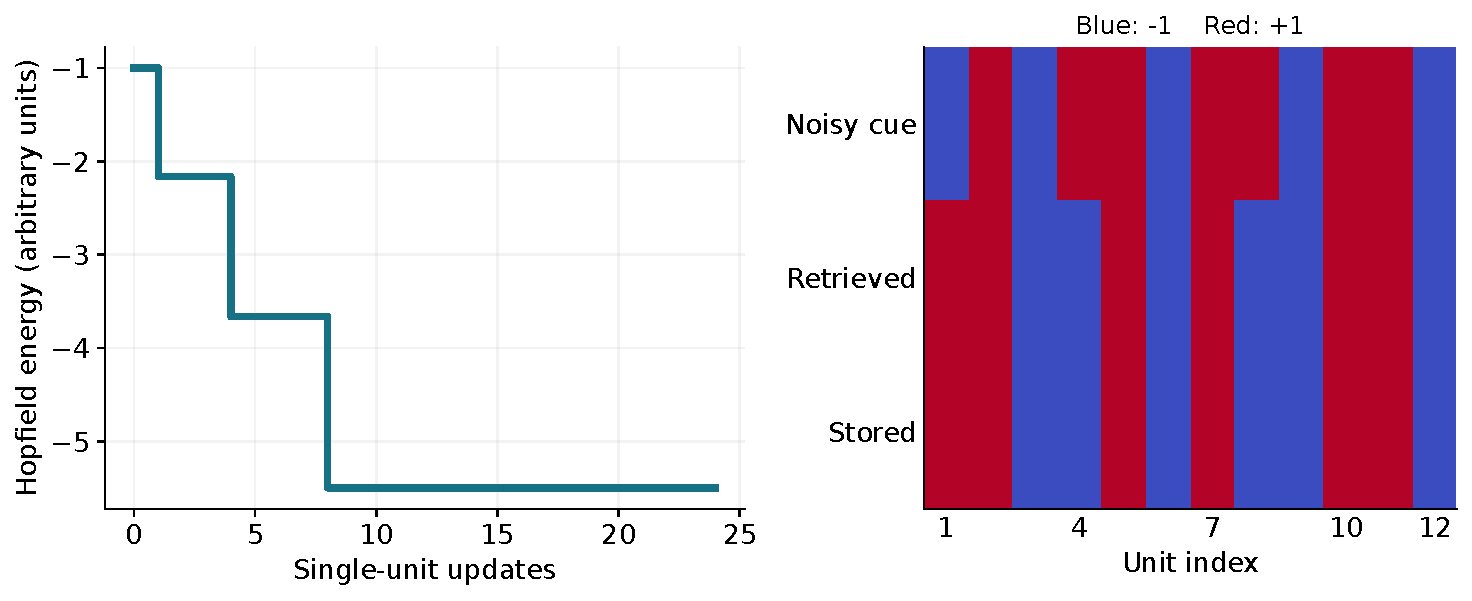
\includegraphics[width=\linewidth]{figures/hopfield.pdf}
\caption{A computed 12-unit Hopfield example with one stored pattern and three flipped bits in the initial cue. The left panel records the energy after individual asynchronous updates; the right panel compares states. The result illustrates associative retrieval under specified assumptions, not human recollection or consciousness. Source code and numeric outputs accompany the paper.}\label{fig:hopfield}
\end{figure}

\begin{table}[htbp]\centering\small
\caption{A vocabulary for careful brain--model comparison. Each row identifies a question rather than a verdict on equivalence.}
\begin{tabularx}{\linewidth}{p{23mm}XX}\toprule
Term & An operational model meaning & What remains to be established \\\midrule
Representation & Information usable by a downstream computation. & Which biological or semantic relationships the representation captures.\\
Attention & Input-dependent weighting in a specified architecture. & Relationship to human selection, control, and awareness.\\
Memory & Parameters, context, retrieval, or stored application state. & Relationship to learning, consolidation, recollection, and selfhood.\\
Reasoning & Performance on inference tasks with explicit tests. & Robustness, mechanism, causal competence, and transfer.\\
Understanding & A stipulated capacity, such as explanation and counterfactual use. & Whether performance supports the intended stronger interpretation.\\\bottomrule
\end{tabularx}\label{tab:vocabulary}
\end{table}

\learningcheck{Parameters, transient context, external retrieval and application records have different update and persistence mechanisms; pattern completion makes one retrieval mechanism explicit.}{A report assistant reproduces a saved preference: which controlled removal would help identify where the preference was supplied?}

\section{Compare systems through controlled tests}\label{sec:comparison}
A brain--model comparison becomes testable when it names an ability and asks which mechanisms could produce it. Searching for a uniquely human remainder by subtracting model successes can obscure this question. If a model succeeds at a task, the result demonstrates that the implemented system is sufficient for that tested behavior under those conditions. It does not establish that its components are necessary for the behavior, or that humans use the same components. If it fails, the cause might be a poor interface, insufficient training, a mismatched task, or a genuine missing capacity.

A stronger protocol therefore starts with a named ability and competing explanations. For example, both a clinician and an image classifier may detect a lesion. One explanation is sensitivity to relevant anatomy; another is reliance on a correlated acquisition cue. Change the cue while preserving the target as far as technically possible, evaluate the change in behavior, and check whether the intervention itself introduces artifacts. Repeat across alternative models and appropriate human comparison groups. Control training exposure and test contamination where feasible, and acknowledge when they cannot be matched.

Agreement in aggregate accuracy is particularly weak evidence for shared mechanisms. Two systems may succeed on different cases, express different uncertainty, or fail for different reasons. Compare error structure, responses to perturbations, and the information available to each system. Ablation can establish dependence on a component within a particular implementation, but the component may be replaceable in a different implementation. These distinctions are also relevant to claims about human-like learning \citep{lake2017}.

\subsection{A transparent shortcut experiment}
Suppose a binary label $Y$ is balanced (half the cases have each label) and a site marker $S$ agrees with it with probability $a$. A shortcut is a predictive cue that works in the development data but need not remain reliable under the intended conditions of use. A fixed rule $\widehat Y=S$ has expected accuracy $a$. Suppose another binary image feature agrees with the label with probability $0.8$, independently of the site--label relation. A fixed feature rule then has expected accuracy $0.8$ under the stipulated changes. At $a=0.95$, the site rule wins. At $a=0.50$, it falls to chance. At $a=0.05$, its predictions are usually wrong. Figure~\ref{fig:shortcut} follows directly from these assumptions; no classifier has been trained and no hospital data have been analyzed.

\begin{figure}[htbp]\centering
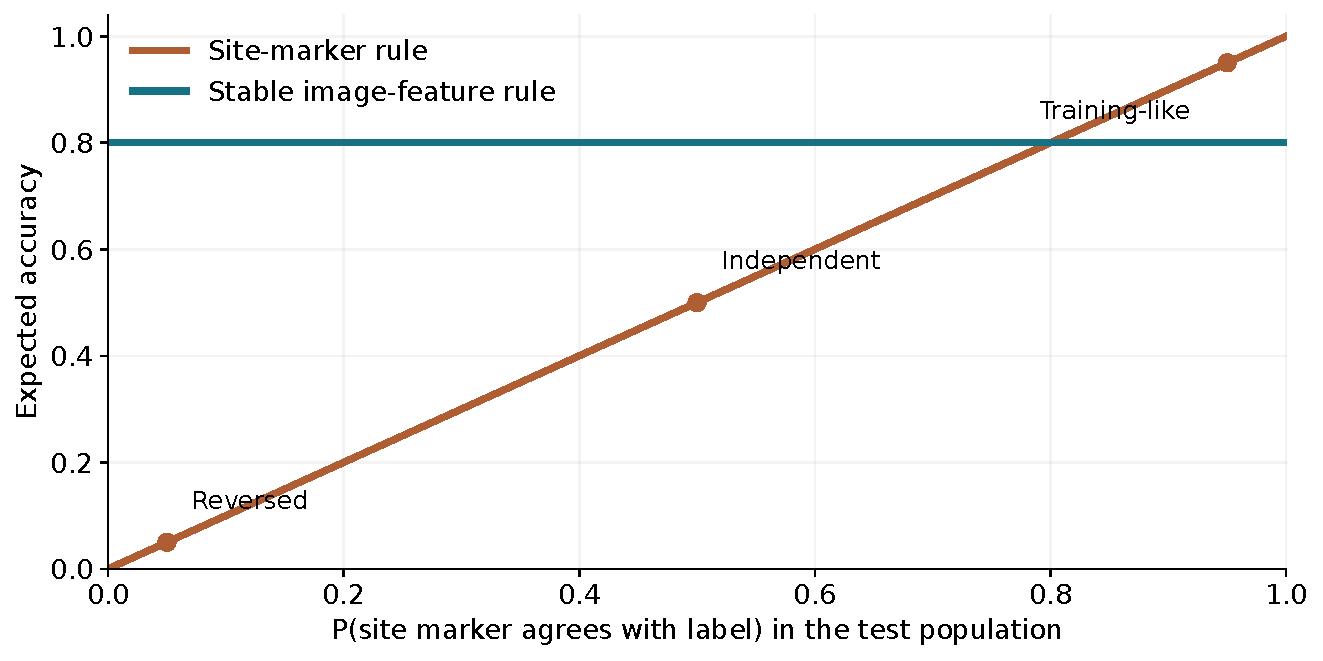
\includegraphics[width=.96\linewidth]{figures/shortcut.pdf}
\caption{Analytic teaching example of shortcut dependence. The site rule's accuracy equals the marker--label agreement probability. The stable feature rule remains at 80\% by construction. The figure illustrates how a ranking can reverse across environments; it does not estimate the performance of a medical AI system.}\label{fig:shortcut}
\end{figure}

The broader shortcut-learning problem is documented across deep learning \citep{geirhos2020}. In chest radiography, cross-hospital evaluation has exposed variable generalization and hospital-associated signals \citep{zech2018}. These findings motivate tests tailored to the proposed shortcut. Keeping each patient entirely within one data partition helps prevent leakage (evaluation information entering development). Site-aware and temporal evaluation test transfer across institutions and time; inspecting acquisition cues tests a proposed source of dependence. A random split alone may leave important correlations untouched. \coursenotebook{11_shortcut_dependence.ipynb}{Notebook 11} reconstructs the three analytic accuracy comparisons.

\learningcheck{A useful comparison changes a suspected cause while controlling alternatives; average accuracy alone leaves many mechanisms compatible with the result.}{The site rule falls from 95\% to 5\% accuracy: which stipulated change produces the reversal?}

\section{Prediction acquires meaning inside a decision}\label{sec:decisions}
A probability is useful when its target and intended use are clear. \emph{Ranking} concerns the order of cases: do cases with the condition tend to receive higher scores? \emph{Calibration} concerns numerical probabilities: among comparable cases assigned a probability near 0.2, does the condition occur about 20\% of the time? \emph{Utility} concerns the consequences of using the output. A model can rank cases well while assigning overly extreme probabilities. Calibration methods can improve probability estimates on suitable evaluation data \citep{guo2017}; calibration should also be checked in the intended population, with uncertainty and subgroup sample size reported.

\subsection{Count the positive results before using the formula}
For a specified target condition and classification threshold, \emph{sensitivity} is the fraction of condition-present cases classified positive. \emph{Specificity} is the fraction of condition-absent cases classified negative. \emph{Prevalence} is the fraction of the population with the condition. \emph{Positive predictive value} (PPV) asks the reverse question from sensitivity: among positive results, what fraction have the condition?

Consider 10,000 hypothetical people with 1\% prevalence, 90\% sensitivity and 90\% specificity. First, $0.01\times10{,}000=100$ have the condition and 9,900 do not. Next, sensitivity gives $0.9\times100=90$ true positives. The false-positive fraction is $1-0.9=0.1$, giving $0.1\times9{,}900=990$ false positives.

\begin{center}\begin{minipage}{\linewidth}\centering
\captionof{table}{Expected counts in the hypothetical 10,000-person example. Rows group people by condition status; columns group them by the classifier's result.}
\begin{tabular}{lrrr}\toprule
Condition status & Positive result & Negative result & Total \\\midrule
Present & 90 & 10 & 100 \\
Absent & 990 & 8,910 & 9,900 \\\midrule
Total & 1,080 & 8,920 & 10,000 \\\bottomrule
\end{tabular}
\end{minipage}\end{center}

There are $90+990=1{,}080$ positive results, so $\mathrm{PPV}=90/1{,}080\approx8.3\%$. The low prevalence supplies many more opportunities for false positives than true positives. This explains why ``90\% accurate'' cannot substitute for a specified performance measure and population.

The same counting argument gives Bayes' formula. In a population of size $N$, the expected true-positive count is $N\,\mathrm{Se}\,\pi$ and the expected false-positive count is $N(1-\mathrm{Sp})(1-\pi)$, where $\pi$ is prevalence, $\mathrm{Se}$ sensitivity and $\mathrm{Sp}$ specificity. Dividing true positives by all positives cancels $N$:
\begin{equation}
\operatorname{PPV}=\frac{\mathrm{Se}\,\pi}{\mathrm{Se}\,\pi+(1-\mathrm{Sp})(1-\pi)}.
\end{equation}
Keeping sensitivity and specificity at 90\%, PPV is 50\% at 10\% prevalence and 90\% at 50\% prevalence (Figure~\ref{fig:ppv}). These are hypothetical calculations. The fixed sensitivity and specificity assumption isolates the effect of prevalence; case mix and acquisition can also change those quantities in practice.

\begin{figure}[htbp]\centering
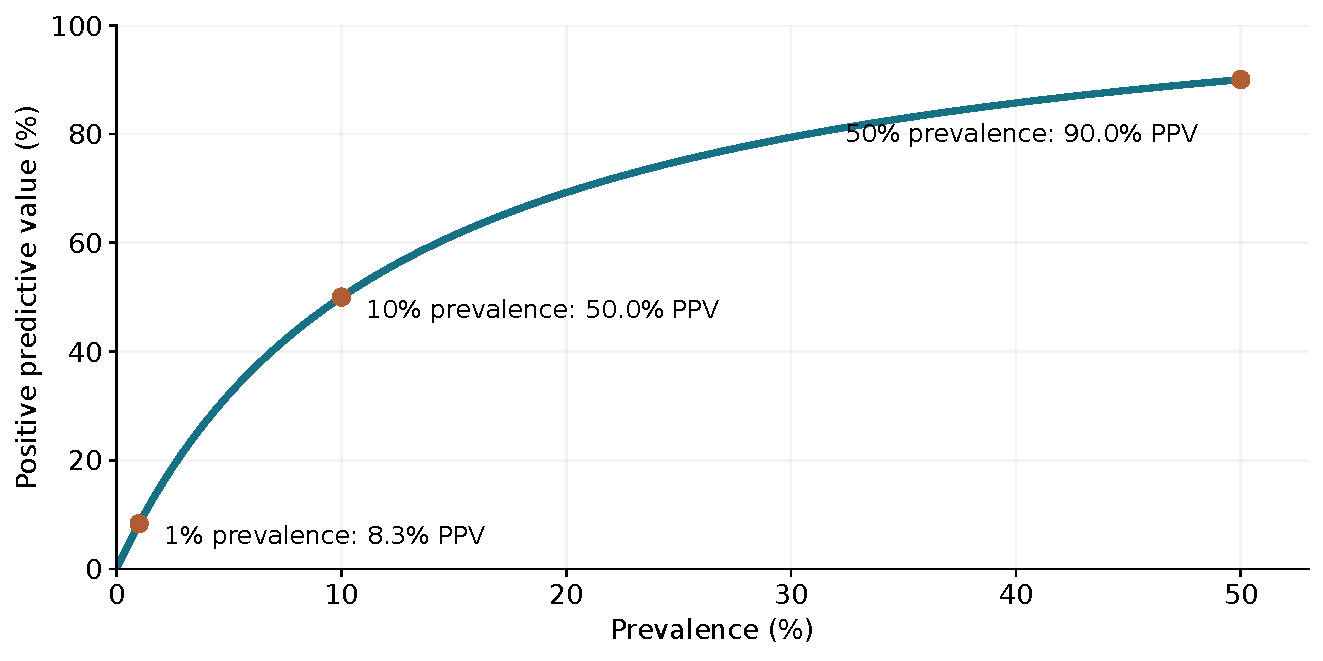
\includegraphics[width=.96\linewidth]{figures/ppv.pdf}
\caption{Positive predictive value under fixed 90\% sensitivity and 90\% specificity. The plotted values are calculated from Bayes' rule. Changing prevalence changes the meaning of a positive classification even before considering calibration drift or altered test performance.}\label{fig:ppv}
\end{figure}

\subsection{Compare the expected consequences of acting}
Let $p$ be the probability of the target condition given the available evidence, used as the decision probability in this simplified model. Let $C_{\mathrm{FP}}$ be the cost of acting when the condition is absent and $C_{\mathrm{FN}}$ the cost of not acting when it is present. If correct actions have zero cost, the expected costs are
\[
L_{\mathrm{act}}=(1-p)C_{\mathrm{FP}},\qquad L_{\mathrm{no\ act}}=pC_{\mathrm{FN}}.
\]
Choose the action when its expected cost is lower. For positive costs, rearrange $(1-p)C_{\mathrm{FP}}<pC_{\mathrm{FN}}$ to obtain
\begin{equation}
p > \frac{C_{\mathrm{FP}}}{C_{\mathrm{FP}}+C_{\mathrm{FN}}}.
\end{equation}
For an arithmetic example, if a missed condition costs four units and an unnecessary action costs one, the threshold is $1/(1+4)=0.2$. These stipulated costs demonstrate the calculation. A clinical decision model would also need justified estimates of treatment harms, delays, competing outcomes, repeated tests and patient preferences. The mathematical point is that an objective does not specify its own acceptable consequences. Someone must justify the target, the actions, and the values represented by their costs.

\coursenotebook{15_ppv_and_decisions.ipynb}{Notebook 15} reproduces the counts and cost comparisons, with separate controls for population rates, decision probability and costs.

\begin{perspectives}{predictive value and decisions}
\textbf{Biomedical and imaging perspective.} Use the 10,000-person table to explain why only 90 of 1,080 positive results are true positives in this example. Identify the population to which those counts refer. Before proposing an action, ask which consequences and patient preferences the simplified cost model leaves out.

\textbf{Computational perspective.} Reconstruct the expected counts and cancel the population size to obtain PPV. Keep population prevalence $\pi$ distinct from the decision probability $p$. Derive the action threshold by comparing the two expected costs, then ask whether the probabilities are calibrated in the population where the rule will be used.
\end{perspectives}

\subsection{Evaluate the system people actually use}
A workflow may change who sees a case, when they see it, and what they believe before reviewing the image. A nominal human checkpoint does not establish effective oversight. The reviewer needs relevant information, sufficient time, the ability to challenge an output, and an actionable fallback. Performance should be assessed for the combined human--AI process, including errors introduced or amplified by that process.

Clinical studies can investigate this process directly. The MASAI randomized mammography screening study illustrates evaluation of an AI-supported reading workflow rather than a model in isolation \citep{masai2023}. Its findings should be interpreted within the intervention and endpoints studied, not generalized to every imaging modality. Reporting guidance provides complementary structure: STARD-AI addresses diagnostic accuracy studies, DECIDE-AI early live clinical evaluation, and TRIPOD-LLM studies involving large language models \citep{stard2025,decide2022,gallifant2025}. A completed checklist is not evidence of benefit; it makes the design and evidence easier to assess.

\begin{table}[htbp]\centering\small
\caption{Moving from a technical result to justified clinical reliance. These are examples of evidence questions, not a certification checklist.}
\begin{tabularx}{\linewidth}{p{28mm}XX}\toprule
Claim & Evidence to examine & What it does not establish alone \\\midrule
A mask is accurate & Relevant reference labels; overlap and boundary errors; small-lesion failures. & Correct diagnosis, response assessment, or treatment benefit.\\
A score transports & External, temporal, and subgroup evaluation; calibration and missing-input behavior. & Utility at the intended action threshold.\\
A report is clearer & Fidelity, omissions, uncertainty preservation, and reader comprehension. & Appropriate advice or improved outcomes.\\
Oversight works & Observed review behavior, correction, workload, escalation, and fallback. & That a nominal human checkpoint prevents harm.\\
The system helps & Prospective workflow comparison and outcomes appropriate to intended use. & Durability after model, population, or workflow changes.\\\bottomrule
\end{tabularx}\label{tab:evidence}
\end{table}

\learningcheck{A positive result depends on prevalence and test performance; an action also depends on justified consequences and the workflow.}{In the 10,000-person example, what happens to false positives and PPV if specificity rises while prevalence and sensitivity stay fixed?}

\section{Research extension: observing reasoning and brain representations}\label{sec:research}
The core examples have distinguished an output from the mechanism producing it. This extension applies the same question to language-model reasoning and brain imaging. It examines representations and algorithms in Marr's framework: what can be observed, what can be decoded from that observation, and what further test would show that a candidate representation contributes to an output?

\subsection{Model interfaces and the observability of reasoning}
An interface specification describes available inputs, outputs and resource limits of a large language model (LLM) application. A long context window specifies how much input may be available to a computation; it does not establish reliable recall of every item or autobiographical memory. Reproducible experiments should record the model version, application configuration, prompts and tools separately from claims about internal architecture or measured performance.

A chain of thought is a sequence of generated intermediate reasoning steps, usually expressed in text. Monitoring it raises a different question: can an observable reasoning trace help detect a specified property of the computation or resulting action? A trace may supply useful evidence, but it is not a complete record of internal activity. Research on monitorability emphasizes that relevant computation may remain unexpressed, and that changes in training or reasoning methods can weaken this source of evidence \citep{korbak2025}. A displayed explanation or summary should also be distinguished from the underlying trace available to an evaluator.

The underlying computational ideas have primary research examples. \emph{Coconut} abbreviates \emph{Chain of Continuous Thought}: it is a method for reasoning through numerical hidden states rather than emitting a natural-language token at every intermediate step \citep{hao2024}. Its last-layer hidden state---a vector of activations---is fed back as the next input embedding. Training progressively replaces explicit reasoning steps with such latent steps; ordinary token generation can resume to produce an answer. This is a particular model-and-training procedure, not a name for every recurrent network.

Recurrent-depth models instead apply an internal block repeatedly, allocating additional computation before producing an output token \citep{geiping2025}. A schematic description is
\begin{equation}
 h^{(k+1)}=F_\theta\!\left(h^{(k)},x\right),\qquad k=0,\ldots,K-1.
 \label{eq:latent-loop}
\end{equation}
Here $x$ denotes the encoded task input or conditioning context; $h^{(k)}\in\mathbb{R}^{d}$ is the numerical latent state after internal step $k$; $d$ is its dimension; $F_\theta$ is the update operation with learned parameters $\theta$; and $K$ is the number of internal updates. The superscript $(k)$ indexes an iteration, not a power. The initial state $h^{(0)}$ is supplied by the model's initialization or input-processing stage. The parameters are held fixed during this schematic inference loop. An actual transformer may maintain a sequence of vectors and cached context, so the equation suppresses implementation details. By contrast, an external text loop decodes and appends tokens between steps. Both can supply additional inference-time computation; neither establishes a human-readable inner language or identifies the architecture of a proprietary system.

\subsection{From fMRI representations to interpretation and understanding}
Functional MRI (fMRI) and language-model monitoring both require an observation to be interpreted through a model, but they expose different kinds of evidence. The blood-oxygen-level-dependent (BOLD) fMRI signal measures haemodynamic changes related to neural activity, rather than individual neural spikes \citep{logothetis2001}. Its spatial pooling and delayed temporal response constrain inferences about rapid processing. A chain-of-thought trace is generated symbolic output; an activation probe reads numerical states when these are accessible. Neither channel becomes an explanation simply because an investigator can decode information from it.

Three operations should be distinguished. An \emph{encoding model} predicts measured brain responses from stimulus features, for example contextual language-model embeddings. A \emph{decoder} predicts stimulus content or a report from brain measurements. An \emph{explanatory test} asks whether a proposed feature or mechanism survives a discriminating experiment. For encoding, independent test stories or images are essential, with temporal alignment and feature selection fitted without test leakage. For decoding, comparisons with language-only, image-only, shuffled-input, and zero-input controls establish what the brain signal adds. For explanation, new stimuli or targeted interventions must challenge alternatives. Similar representational geometry is evidence of a relationship under a chosen analysis, not proof of identical computation.

A foundational example is \citet{tang2023}: their fMRI decoder generated language capturing aspects of perceived and imagined speech and silent-video content. Its dependence on participant cooperation illustrates why successful decoding in a trained setting should not be generalized to unrestricted access to thought. More recent work extends the comparison in several directions. The following studies illustrate different tests of representation and interpretation.

\paragraph{Visual meaning in a language-model space.}
\citet{doerig2025} showed that embeddings of scene captions predict fMRI responses to viewed scenes and support caption reconstruction. Controlled comparisons implicated contextual information beyond individual words; image networks trained to predict these embeddings also acquired representations aligned with brain responses. This provides a quantitative account of some high-level visual information, while leaving open whether humans use the model's representational format or learning procedure.

\paragraph{Readable hypotheses tested in the scanner.}
\citet{antonello2026} developed \emph{generative causal testing}: descriptions of what drives a brain-response model are used to generate new linguistic stimuli, and the resulting brain responses test those descriptions. The method connects prediction to experimentally tested selectivity. Manipulating stimulus content strengthens an explanation of response tuning, but does not by itself identify a necessary neural circuit or explain subjective understanding.

\paragraph{Sparse features and competing predictors.}
In the cited preprint, \citet{lepori2026} replaced dense language-model states with sparse-autoencoder features (a learned representation that uses relatively few active components) and included surprisal as a separate predictor. Surprisal is $-\log P(w\mid\text{context})$: an unlikely word $w$ has greater surprisal. Using 7-T fMRI from eight participants listening to 200 sentences, they identified interpretable response profiles, including sensitivity to people-related content; frontal responses were relatively well explained by surprisal alone. This is a useful bridge between model interpretation and brain encoding, and a reminder to test simpler predictors before attributing explanatory power to a complex embedding.

\paragraph{Inner speech and the contribution of context.}
The \emph{MindAlign} preprint maps fMRI during silent image description into a semantic space (a vector representation of meaning-related distinctions), then combines that representation with visual context to prompt a frozen multimodal language model \citep{liu2026mindalign}. The authors report improvements over fMRI-only and random baselines. Because the image supplies information about the intended description, the central explanatory question is what neural input adds beyond an image-only account. The trained task should not be equated with unconstrained inner-speech reading.

\paragraph{A recent decoding failure that sharpens the test.}
The preprint by \citet{suvakovic2026} reports that apparently strong candidate-ranking performance in an fMRI-to-language system remained essentially unchanged when fMRI inputs were zeroed. The result is specific to their system and evaluation; it does not invalidate neural decoding generally. It does show why fluent output and above-chance ranking cannot establish brain-signal use without appropriate controls. Their decoding regimes and test stories also differ across comparisons, limiting broad performance conclusions.

These studies suggest a concrete connection to monitoring LLM inference. A probe can reveal that information is available in a hidden state, just as a decoder can recover information from fMRI; demonstrating that the system \emph{uses} that information requires further evidence. In an accessible model, activation replacement, ablation, or a controlled input change can test whether the candidate representation contributes to an output. In a person, experimentally varied stimuli, behavioural measurements, and appropriately justified neural interventions answer related but non-identical questions. A readable reasoning trace, an activation-based interpretation, and an fMRI reconstruction should therefore be evaluated against a specified target, such as detecting an error or distinguishing two hypotheses, rather than treated as interchangeable windows into thought. Understanding advances when the proposed account predicts what will change under a new test.

\learningcheck{Decoding information and demonstrating its contribution to an output require different tests.}{If candidate-ranking performance is unchanged after fMRI inputs are zeroed, what contribution of the brain signal has that evaluation established?}

\section{Embodiment and viability: a hypothesis with limits}\label{sec:embodiment}
A useful introduction is the family of \emph{4E approaches}: cognition is considered as embodied, embedded, enactive, and extended \citep{newen2018}. Embodied emphasizes bodily contributions; embedded emphasizes environmental and social supports; enactive emphasizes cognition through active engagement; extended asks whether some tightly integrated external resources constitute parts of a cognitive process. These approaches overlap, but they are not one theory with a single test. Appendix~\ref{app:4e} develops the distinctions through the imaging vignette.

For this paper, their value is to broaden the unit of analysis. A clinician's interpretation depends on a body, a working environment, active inspection, and external records. Whether an external resource merely supports cognition or partly constitutes it is a further philosophical claim \citep{clark1998}. Workflow dependence can be studied without first deciding that stronger question.

A substantive philosophical proposal concerns prediction under viability constraints: the conditions an organism must maintain to remain alive. Biological cognition occurs in organisms that regulate bodily conditions, develop over time, act in an environment, and can be injured. This gives perception and action a practical significance that is not captured by a task score alone. Predictive and interoceptive accounts (concerning sensing and regulation of internal bodily conditions) make aspects of this proposal computationally explicit \citep{friston2010,seth2013}.

The proposal should not be inflated into the claim that all behavior is governed by a single literal survival objective. People pursue social, intellectual, moral, and self-destructive goals. Nor is embodiment uniquely human: it characterizes many living systems. Calling it the human remainder would therefore confuse a contrast with certain engineered systems and a definition of humanity. The defensible claim is that bodily regulation and lived context deserve explicit consideration when interpreting human cognition and clinical needs.

The artificial side needs equal care. A base language model's next-token training objective is not a complete description of every deployed AI system. Post-training, multimodal input, retrieval, external tools, memory, and robotic interaction alter the system being evaluated. Some artificial systems act through bodies and feedback loops. Being embodied in an engineering sense does not itself settle whether a system has biological needs or experience. Conversely, the absence of biological metabolism is not a proof that experience is impossible.

A more precise comparison therefore names the systems: for example, an adult human regulating bodily state and a specified language-model application with fixed weights, a given context window, and defined tools. It asks which feedback signals are available, what changes through learning, how goals are represented, and what counts as failure. These questions can be investigated without first settling a universal boundary between humans and machines.

\learningcheck{Body, environment and feedback can change the appropriate unit of analysis; a proposed role should be tied to an observable comparison.}{How would you distinguish an effect of active image exploration from an effect of seeing different images?}

\section{Consciousness: experience, access and evidence}\label{sec:consciousness}
``Consciousness'' can name different explanatory targets. Here, \emph{phenomenal consciousness} means subjective experience: there being something it is like to see a colour, feel pain, or hear a sound. \emph{Access consciousness} concerns information being available for use in reasoning, report, and deliberate control \citep{block1995}. The first asks about experience; the second asks about availability for cognitive use. These are conceptual distinctions, not two established anatomical compartments.

Consider seeing a red warning on a display. Its visual appearance illustrates the phenomenal question. Using the warning to explain a concern or decide what to inspect next illustrates the access question. The example distinguishes questions about an ordinary event; it does not demonstrate that the two properties can be cleanly separated experimentally. Wakefulness, selective attention, self-awareness, and verbal report are also relevant concepts, but none should be used as a synonym for all consciousness.

Global neuronal workspace theory proposes that information becomes widely available through interactions among specialized processors. Such broadcasting is a proposed mechanism for aspects of conscious access; it is not simply a restatement of the definition. Integrated information theory makes different commitments about the causal organization relevant to experience \citep{sethbayne2022}. A theory, a measured correlate, and a definition must therefore be kept distinct when interpreting experiments.

An AI system can produce a sentence about pain, uncertainty, or self-awareness. The sentence is an observable output. Whether it provides evidence of experience depends on additional assumptions about the system and the relation between report and consciousness. The same caution applies to the reverse inference: inability to give a verbal report does not show absence of experience. This matters in medicine, where patients may have impaired communication.

An adversarial collaboration, in which proponents of competing theories agree on tests, examined predictions of global neuronal workspace and integrated information theories \citep{cogitate2025}. It does not establish a universally accepted test for consciousness in artificial systems. Theory-derived indicator approaches offer a structured way to assess AI while retaining uncertainty about both the theories and their application \citep{butlin2025}.

Two positions deserve a fair hearing. A functionalist approach holds that relevant organization could, in principle, be implemented in more than one substrate. A biologically oriented approach argues that details of living organization may matter in ways current models omit. Neither position is resolved by a fluent conversation or by showing that a model uses matrix multiplication. The purpose of the keynote is to explain why the question remains open and how stronger evidence might be sought, not to announce that consciousness has been detected or excluded.

There is also an ethical distinction between determining a machine's possible moral status and determining its effect on people. A nonconscious system could profoundly alter a patient's care, expectations, or opportunities. Clinical responsibility therefore cannot wait for agreement about machine experience. People and institutions remain the parties who select, deploy, oversee, and respond to the consequences of clinical systems.

\learningcheck{Experience, access, report and proposed mechanisms are different explanatory targets.}{A model accurately reports information from an earlier input: which observation concerns access, and what additional argument would be needed to infer experience?}

\section{A report exercise that bridges into RadKom}\label{sec:report}
The RadKom workshop on patient-friendly radiology language provides a practical setting for this exercise. Consider the invented sentence: \emph{``The enhancement is indeterminate; treatment-related change and progression remain possible.''} Ask participants to produce a plain-language rendering while preserving both possibilities and the uncertainty.

A reasonable answer is: \emph{``The scan shows a change whose cause is not yet clear. It may be related to treatment, or it may mean the tumour has grown.''} The source supplies two possible causes and no definite plan. The rendering preserves those possibilities without adding a diagnosis, treatment recommendation or promised follow-up.

A technically fluent model may make the passage shorter and warmer while changing its meaning. An expert may preserve meaning while using language that is hard to understand. These are separate dimensions and should be evaluated separately. In Marr's terms, preserving clinically relevant meaning is the task, the wording and transformation procedure are the representation and algorithm, and the particular model/application supplies the implementation. Record the input, exact model or system version, prompt, output, and human revisions. Reviewers assess contradiction, unsupported additions, omissions, uncertainty, and readability. Patient or public involvement should shape what counts as understandable communication in the intended setting.

This example also connects to a linguistic debate. Bender and Koller distinguish linguistic form from meaning and caution against unexamined claims of understanding \citep{bender2020}. Their argument concerns the relationship between a learning setup and a stronger semantic claim; it should not be turned into a blanket empirical verdict on all multimodal or interactive AI. For this exercise, the operational question is more tractable: did the transformation preserve the source's clinically relevant propositions and their uncertainty?

\learningcheck{Plain language should preserve the source propositions and their uncertainty while making them easier to understand.}{Does replacing ``may mean the tumour has grown'' with ``the tumour has grown'' preserve the source meaning?}

\section{Teaching transferable judgment}\label{sec:teaching}
A mixed cohort benefits when each technical concept ends in an interpretable question. After the attention example, ask what operation it implements; use Appendix~\ref{app:attention} for the calculation. After the Hopfield example, ask which assumptions ensure energy decreases. After the shortcut plot, ask which test would distinguish useful anatomy from acquisition cues. After the prevalence calculation, ask what additional information is needed before acting. The same activity can be approached computationally by one participant and conceptually by another.

Use the perspective boxes for a paired explanation: one reader explains what a result could mean for an observation or decision, and another reconstructs the calculation and its assumptions. Exchange roles before proposing a further test. Both readers should be able to state what was computed and which interpretation the evidence supports.

The educational aim is not simply to teach students how to obtain an answer from a model. It is to make them specify what they would accept as evidence and notice when an answer exceeds that evidence. A practical assessment can ask students to submit a result together with one falsification attempt: a changed population, a perturbed input, a contradictory example, or a check of the source text. An unsuccessful model can still teach something if the failure is characterized accurately; a successful one can still be misunderstood.

The accompanying code uses small deterministic examples that run on an ordinary CPU. No large-model download is required. Keeping the demonstrations modest supports inspection and reproducibility. For substantive model experiments, resource reporting should name the model, precision, context, software, workload, and measurement method. Memory estimates for weights alone exclude runtime buffers and other overhead.

A useful collaboration between the two school communities would pair a computational claim with a conceptual audit. One participant states the target, data, and test. Another asks what the target leaves out, whose purposes it serves, and which stronger interpretations might be mistakenly inferred. Both then revise the experiment. This is not an opposition between engineering and ethics; the questions jointly determine whether the technical result is relevant to the proposed use.

\learningcheck{An informative exercise reports both a result and an attempt to challenge its interpretation.}{Choose one notebook result: which alternative explanation would your next controlled test address?}

\section{Conclusion}\label{sec:conclusion}
AI can serve as a comparative instrument for studying human abilities and as a practical instrument for medicine. Its value in both roles increases when the claims become narrower and more testable. Shared outputs do not by themselves imply shared mechanisms. Shared terminology does not settle shared experience. A successful model needs a justified connection to the actions people take with it.

The most useful conclusion for clinical integration is therefore a disciplined allocation of questions. Ask the model what it can estimate under specified conditions. Ask the experiment which alternative explanations have been excluded. Ask the clinical team and patient what matters for the decision. Being human need not be defined as whatever the latest model cannot yet do. In medicine, our responsibilities become clearer when we understand both the power of these models and the lives into which their outputs enter.

\learningcheck{Specify the computation, test competing explanations, and connect the result to the purposes of the people using it.}{For a model claim you encounter next, what single observation would make you revise your interpretation?}

\section*{Reproducibility and provenance}
The training examples and simulated tumour states are generated for teaching; the glioma and fMRI studies are empirical research identified separately. Reproduced figures contain published LUMIERE case information; no patient imaging volumes or additional patient records are distributed here. The normal BrainWeb T1 phantom and tissue labels used in Notebooks 14b/14c are bundled with the code, with source attribution and checksums. The \href{https://github.com/arvidl/brains-to-models/blob/main/talk/resources.md}{presentation guide} maps topics to local notebooks and versioned external implementations. The \href{https://github.com/arvidl/brains-to-models/blob/main/code/notebooks/README.md}{notebook guide} supplies learning goals, setup instructions and Colab links. AI assistance was used in preparing text and code; scientific interpretation and responsibility rest with the named author. Source, dependencies and reproduction commands are recorded in \url{https://github.com/arvidl/brains-to-models}. A short \href{https://github.com/arvidl/brains-to-models/blob/main/paper/background/README.md}{repository note} documents the preserved background manuscript.

\FloatBarrier
\appendix
\section{Attention: from similarity scores to a weighted output}\label{app:attention}
\subsection{The operation and its dimensions}
For one attention head, let $X\in\mathbb{R}^{n\times d_{\mathrm{model}}}$ contain $n$ token or image-patch representations, one per row. The notation $\mathbb{R}^{n\times d}$ means a matrix of real numbers with $n$ rows and $d$ columns; $d_{\mathrm{model}}$ is the number of features per representation. Learned projection matrices give $Q=XW_Q$, $K=XW_K$, and $V=XW_V$, with $Q,K\in\mathbb{R}^{n\times d_k}$ and $V\in\mathbb{R}^{n\times d_v}$. Thus $d_k$ is the query/key dimension and $d_v$ the value dimension. A superscript $\top$ denotes transpose, exchanging rows and columns. Scaled dot-product attention is
\begin{equation}\label{eq:attention}
 A=\operatorname{softmax}_{\mathrm{row}}\!\left(\frac{QK^\top}{\sqrt{d_k}}+M\right),
 \qquad Z=AV.
\end{equation}
The $n\times n$ matrix $A$ contains normalized weights; $Z$ has shape $n\times d_v$. For scores $s_{ij}$, row-wise softmax computes $A_{ij}=e^{s_{ij}}/\sum_\ell e^{s_{i\ell}}$: exponentiate each score and divide by the total in its row. An optional mask $M$ excludes disallowed positions by adding $-\infty$ to their scores, making their exponential zero; allowed positions receive zero in $M$. With finite allowed scores and at least one allowed key, each row of $A$ sums to one. Causal masking prevents access to later positions when predicting a sequence one token at a time. In cross-attention, queries and keys/values come from different sequences and $A$ need not be square \citep{vaswani2017}.

\subsection{An original two-key calculation}
Take one query $q=(1,0)$, two keys $k_1=(1,0)$ and $k_2=(0,1)$, and scalar values $v_1=2$, $v_2=10$. With $d_k=2$ and no mask, the scores are $z_1=1/\sqrt{2}$ and $z_2=0$. Thus
\begin{align}
\alpha_1&=\frac{e^{1/\sqrt{2}}}{e^{1/\sqrt{2}}+1}\approx0.6698,
&\alpha_2&\approx0.3302,\\
o&=\alpha_1\,2+\alpha_2\,10\approx4.6419.
\end{align}
The larger match receives more weight, but the other value still contributes. If both scores were equal, the output would be their average, 6. If only the first key were allowed by the mask, the output would be 2. These are consequences of this toy calculation, not measurements from a trained model.

The weights alone do not determine the output. Keeping the same query and keys while changing $v_2$ from 10 to $-10$ leaves the displayed attention weights unchanged, yet changes the output from about 4.6419 to $-1.9629$. This is a simple counterexample to treating a weighting plot as a complete explanation of the computation. The example is reproduced in \texttt{code/src/brainsmodels/clinical\_appendix.py}.

To check the intermediate arithmetic, $e^{1/\sqrt{2}}\approx2.0281$, so the weights are approximately $2.0281/3.0281$ and $1/3.0281$. Using the unrounded weights, their contributions to the original output are $\alpha_1v_1\approx1.3395$ and $\alpha_2v_2\approx3.3024$. The second value contributes more despite its smaller weight. In the intervention, only the sign of that second contribution changes. \coursenotebook{10_two_key_attention.ipynb}{Notebook 10} performs the calculation at full precision.

Why divide by $\sqrt{d_k}$? Under the illustrative assumptions that query and key components are independent, zero-mean, and unit-variance, their dot product has variance $d_k$. Scaling gives variance one. Large unscaled scores can concentrate softmax weights and reduce its local sensitivity. This calculation motivates the scale; it does not assert that trained representations meet those distributional assumptions exactly \citep{vaswani2017}.

Multiple heads apply different projections and their outputs are combined. A full Transformer also has other operations, including feed-forward transformations and residual paths. Accordingly, an attention matrix describes one intermediate operation. It neither identifies human attentional mechanisms nor by itself establishes which input features causally determine the final prediction.

\subsection{Executable maps from one self-attention sublayer}\label{app:maps}
The accompanying NumPy exercise uses 16 synthetic image patches and one summary token (CLS). Each row of $X\in\mathbb{R}^{17\times4}$ contains an intensity, two position coordinates, and a CLS indicator. The projection matrices are explicitly specified in the code. They are not fitted to data. The sublayer and scalar output are
\[
Q=XW_Q,\quad K=XW_K,\quad V=XW_V,\qquad
Y=X+AVW_O,\qquad f(X)=Y_{0,:}w.
\]
Here $W_Q,W_K\in\mathbb{R}^{4\times2}$, $W_V,W_O\in\mathbb{R}^{4\times4}$, and $w\in\mathbb{R}^{4}$. Attention uses Equation~\ref{eq:attention} without a mask. The residual path is retained, but layer normalization, a feed-forward block, multiple heads, and training are omitted so that every dependency is inspectable. This is the attention operation used within a Transformer, not a complete trained Transformer. The output $f$ is an arbitrary score, not a clinical probability.

Three maps are computed for this same output. The attention map is the CLS row $A_{0,1:17}$ reshaped onto the patch grid; the CLS self-weight is omitted without renormalization. The signed gradient is $\partial f/\partial X_{j,0}$: it measures local sensitivity to patch intensity while holding position fixed. The occlusion effect is $f(X)-f(X^{(j\leftarrow b)})$, where only patch $j$'s intensity is replaced by baseline $b$. A positive gradient means a sufficiently small intensity increase raises the score. A positive occlusion effect means the chosen replacement lowers the score. The two need not agree in magnitude or ranking because occlusion is a finite change and depends on the baseline.

\begin{figure}[htbp]\centering
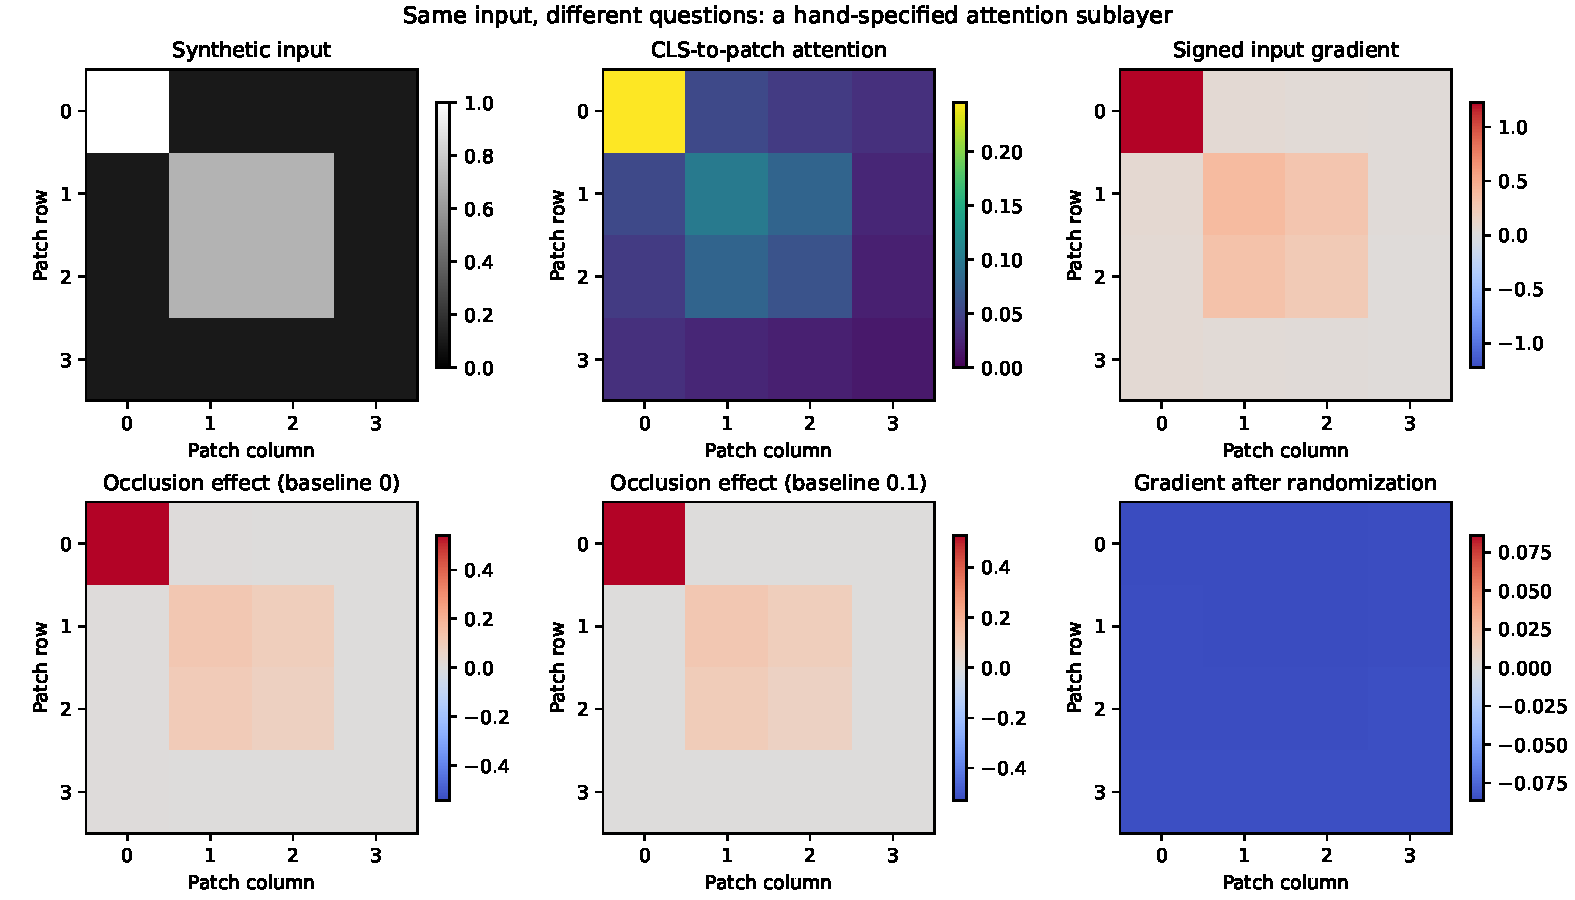
\includegraphics[width=\linewidth]{figures/attention_maps.pdf}
\caption{Computed maps from the same hand-specified self-attention sublayer. The central square is a synthetic pattern and the upper-left patch is a marker. Each panel has its own numerical scale: colours across panels are not directly comparable. The lower row compares two occlusion baselines and a gradient after parameter randomization. These are illustrative computational quantities, not anatomical explanations.}\label{fig:maps}
\end{figure}

For the supplied input, $f=1.586054$. Replacing the upper-left marker intensity 1.0 by the background value 0.1 leaves the central pattern unchanged and gives $f=1.057792$, a decrease of 0.528262. This demonstrates marker sensitivity by construction; it does not demonstrate that training learned a shortcut. In a second intervention, reversing the intensity contribution to the values leaves attention weights exactly unchanged but gives $f=-1.457165$. Thus the same attention display can accompany different outputs. Replacing all parameter arrays with seeded random draws supplies a further parameter-dependence illustration. Since no model is trained, this exercise does not implement a training-label randomization test and should not be presented as reproducing \citet{adebayo2018}.

The implementation computes the gradient analytically by the chain rule and verifies every input component against central finite differences with step $10^{-6}$. A central finite difference estimates a derivative by evaluating the output just above and below an input value and dividing the difference by twice the step. The maximum absolute discrepancy in the recorded check was below $10^{-8}$. It also checks row normalization and the unchanged attention matrix in the value-only intervention. The JSON output preserves full matrices, scores, both occlusion baselines, and package versions. After setting up the project environment as described in the repository, run the example from the project root:
\begin{verbatim}
python -m brainsmodels.attention_maps
\end{verbatim}
A notebook calls the same shared implementation in \path{code/notebooks/08_attention_maps.ipynb} with instructions. An extension for students is to change the occlusion baseline or readout while holding everything else fixed and predict which map will change. Applying these methods to a trained clinical system would additionally require a specified model, preprocessing, output target, valid intervention, and independent evaluation data.

\learningcheck{A weighted output depends on scores and values; a gradient and a finite replacement describe different changes to that output.}{If both scalar values equal $-3$, what output must any normalized pair of attention weights produce?}

\section{Hopfield memory: a cue, an update rule, and an energy}\label{app:hopfield}
\subsection{An explicit model of pattern completion}
A stored configuration can act as an attractor: nearby starting states may settle into it. A landscape analogy is helpful if used carefully. A state is a location, the energy is its height, and the update rule restricts the available moves. Descending does not guarantee arrival at the intended valley. The construction below specifies what ``descending'' means, making the analogy checkable rather than explanatory by itself.

Let $s\in\{-1,+1\}^{N}$ be the current state: a vector of $N$ units, each with sign $-1$ or $+1$. For a single target pattern $\xi$ of the same size, define
\begin{equation}
w_{ij}=\frac{\xi_i\xi_j}{N}\quad(i\ne j),\qquad w_{ii}=0,
\qquad E(s)=-\frac12\sum_{i,j}w_{ij}s_i s_j.
\end{equation}
The weights are symmetric. The zero diagonal excludes self-input, and the factor $1/2$ avoids counting each pair twice. This is a classical associative-memory construction motivated by \citet{hopfield1982}; the following calculations spell out the particular teaching example.

For a selected unit $i$, compute its local field $h_i=\sum_jw_{ij}s_j$, the weighted input from the other units. Set $s_i'=+1$ if $h_i>0$, $s_i'=-1$ if $h_i<0$, and retain $s_i$ if $h_i=0$. The prime marks the new value. All other units remain unchanged; this is an asynchronous update. Cycle through the units, repeating until a complete pass makes no changes. The plotting implementation uses two passes for its specified cue, which is sufficient for that example.

\subsection{Why this update cannot increase energy}
Only terms involving $i$ change. Symmetry and the zero diagonal give
\begin{equation}
\Delta E=E(s')-E(s)=-(s_i'-s_i)h_i.
\end{equation}
If the sign stays the same, $\Delta E=0$. If it changes, $s_i'=-s_i$ and $s_i h_i<0$, hence $\Delta E=2s_i h_i<0$. Our tie rule prevents changes at zero field. Thus every actual change strictly decreases energy. With a finite state space and repeated visits to every unit, this rule reaches a fixed point. It need not reach the global minimum or the desired pattern. Simultaneous updates change the argument and can produce cycles; the proof does not apply to arbitrary network dynamics.

\subsection{Connecting the proof to Figure~\ref{fig:hopfield}}
The target in the supplied code is
\[
\xi=(1,1,-1,-1,1,-1,1,-1,-1,1,1,-1).
\]
The cue flips units 1, 4, and 8 (indices 0, 3, and 7 in Python). Write $m=\sum_i\xi_i s_i$ for the unnormalized overlap. For this single-pattern construction,
\begin{equation}
E(s)=-\frac{m^2-N}{2N}.
\end{equation}
Initially $N=12$ and $m=6$, so $E=-1$. After the three incorrect signs are corrected, $m$ takes values 8, 10, and 12, giving energies approximately $-2.1667$, $-3.6667$, and $-5.5$. Updates of already aligned units leave the energy unchanged. These steps explain both the drops and flat segments in the plot.

For the first correction, unit 1 is misaligned with its target: $\xi_1=+1$ and $s_1=-1$. Its local field is $h_1=\xi_1(m-\xi_1s_1)/N=7/12$, so $s_1'=+1$. Substitution into the energy-change formula gives $\Delta E=-(1-(-1))(7/12)=-7/6$. Adding this to the starting energy $-1$ gives $-13/6\approx-2.1667$, matching the first drop in the recorded trajectory.

There is a revealing limitation even here: $-\xi$ has the same minimum energy as $\xi$ and is also stable. Energy minimization alone cannot distinguish the intended pattern from its inverse. With several patterns, one can use $w_{ij}=N^{-1}\sum_\mu\xi_i^\mu\xi_j^\mu$ for $i\ne j$, but interference and additional attractors complicate retrieval. A useful extension exercise is to vary the initial flips and stored patterns, recording which attractor is reached. The energy proof remains valid when its assumptions hold, while retrieval success can change. This separates a proved dynamical property from a claim about memory performance.

\learningcheck{The energy proof concerns an update rule under stated assumptions; retrieval success additionally depends on the cue and stored patterns.}{Why does starting at $-\xi$ give a counterexample to the claim that descending energy always recovers the intended target?}

\section{4E cognition: four questions about the clinical setting}\label{app:4e}
The 4E vocabulary identifies related but distinct emphases \citep{newen2018}. \emph{Embodied} approaches attend to bodily contributions to cognition. \emph{Embedded} approaches attend to its environmental and social setting. \emph{Enactive} approaches emphasize activity and ongoing organism--environment engagement. \emph{Extended} approaches ask whether some external resources can be constituents of cognition. The distinction between a causal influence and a constituent is consequential: showing that a tool changes performance is insufficient, by itself, to establish that it is part of a mind.

The following applications are proposed teaching examples, rather than empirical findings about radiology teams.

\begin{table}[htbp]\centering\small
\caption{Applying the four questions to the hypothetical MRI review. The examples translate concepts into investigable workflow questions.}
\begin{tabularx}{\linewidth}{p{21mm}XX}\toprule
Emphasis & Illustrative question & A possible comparison \\\midrule
Embodied & Does the clinician's bodily state affect sustained inspection and interpretation? & Compare controlled viewing tasks across recorded fatigue or ergonomic conditions.\\
Embedded & How does access to prior scans, team discussion, and the reporting environment shape interpretation? & Compare available information and coordination under specified workflows.\\
Enactive & How does scrolling, changing the view, and revisiting a region alter the evidence obtained? & Compare active image exploration with matched prerecorded viewing.\\
Extended & Does a reliably integrated record function as part of the ongoing reasoning process? & Document patterns of reliance and disruption, while separating performance effects from the constitutive claim.\\\bottomrule
\end{tabularx}
\end{table}

Under suitable functional integration, the extended-mind proposal treats external resources as constituents of a cognitive process \citep{clark1998}. A performance difference with and without a longitudinal record measures dependence on the record; identifying it as a cognitive constituent requires an additional argument.

Specify what each comparison holds constant. Prerecorded viewing can change both agency and visual evidence; withdrawing a record changes task difficulty as well as tool availability. These alternatives need controls, as in the earlier shortcut example.

The four questions broaden the explanation of a clinical decision to include the patient, clinician, tool and environment, each with a proposed observable role.

\learningcheck{A workflow study can measure dependence on a tool while leaving the stronger claim about cognitive constitution open.}{If withdrawing a longitudinal record reduces accuracy, which task-difficulty explanation would you need to examine before making an extended-mind claim?}

% One source thumbnail and two reading paths per teaching page.
\clearpage
\begingroup
\newcounter{courseslide}
\newenvironment{slidenotes}[3]{%
  \ifnum#1=1\relax
    \section{Slide-by-slide syllabus companion}\label{app:slides}
    {\small Read either path, then compare explanations. Thumbnails reproduce the supplied slides unchanged; the notes clarify their interpretation. Slide numbers follow the presentation.}\par
  \else\clearpage\fi
  \begin{center}#3\end{center}\vspace{-2mm}
  \refstepcounter{courseslide}
  \subsection*{Slide #1. #2}\label{app:slide-#1}
  \addcontentsline{toc}{subsection}{Slide #1. #2}
  \small
}{\par}
\newcommand{\biopath}{\par\smallskip\textbf{Biomedical and imaging path}\par\nobreak}
\newcommand{\comppath}{\par\medskip\textbf{Computational path}\par\nobreak}

\begin{slidenotes}{01}{From brains to models}{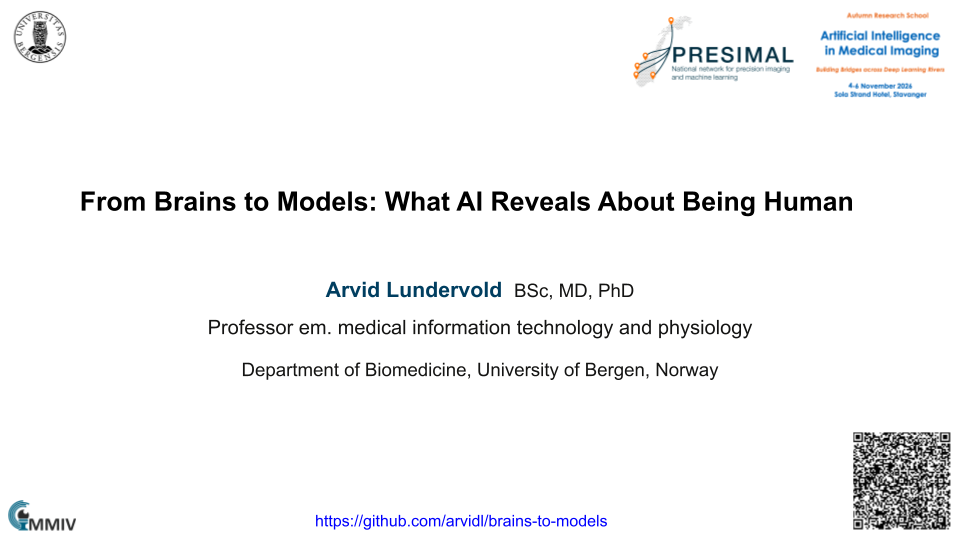
\includegraphics[width=.64\linewidth]{figures/talk/slide-01.png}}
\biopath
The title introduces a comparison between biological cognition and engineered systems. In medicine, the comparison becomes concrete when a model reads an image, produces a lesion outline, or drafts an explanation. Each activity resembles something a professional does, but resemblance leaves several questions open. Does the system detect the relevant tissue? Does it use the same evidence as the professional? Does its output help a patient? A successful answer to one question supplies a starting point for the next investigation.

Use three distinctions throughout this syllabus: performance, mechanism and consequence. Performance concerns what a system achieves under a specified test. Mechanism concerns how it achieves that result. Consequence concerns what happens when people act on it. For example, a more reproducible tumour-volume estimate could improve measurement without yet establishing a treatment benefit. Keep the person whose care is at stake in the account: symptoms, preferences and acceptable burdens are part of the problem being solved. As you work, choose one imaging task and write a sentence for each distinction. Revisit those sentences after the modelling and decision examples.
\comppath
A model is a deliberately selective representation. A neural network represents relationships through learned parameters; a growth equation represents chosen processes through variables and update rules. Both require an account of their inputs, outputs and intended use. Begin by specifying a function, a data-generating setting and an evaluation criterion. A segmentation system, for example, maps an image array to labels. Agreement with a reference mask measures one property of that mapping; it leaves the reference policy and its clinical relevance to be justified.

Brain--model comparisons require equally explicit targets. Similar outputs can arise from different algorithms, and similar internal patterns can support different behaviours. Ask what intervention would distinguish competing explanations: remove a suspected image cue, change the input distribution, or alter a model component while holding the task fixed. \coursenotebook{00_intro_timeline.ipynb}{Notebook 00} introduces this explanatory discipline. Keep a record of the claim, test, result and remaining uncertainty for each exercise. This turns the talk into a sequence of research questions and makes clear which conclusions depend on measurements, stipulated assumptions or philosophical interpretation.
\end{slidenotes}

\begin{slidenotes}{02}{A learning programme}{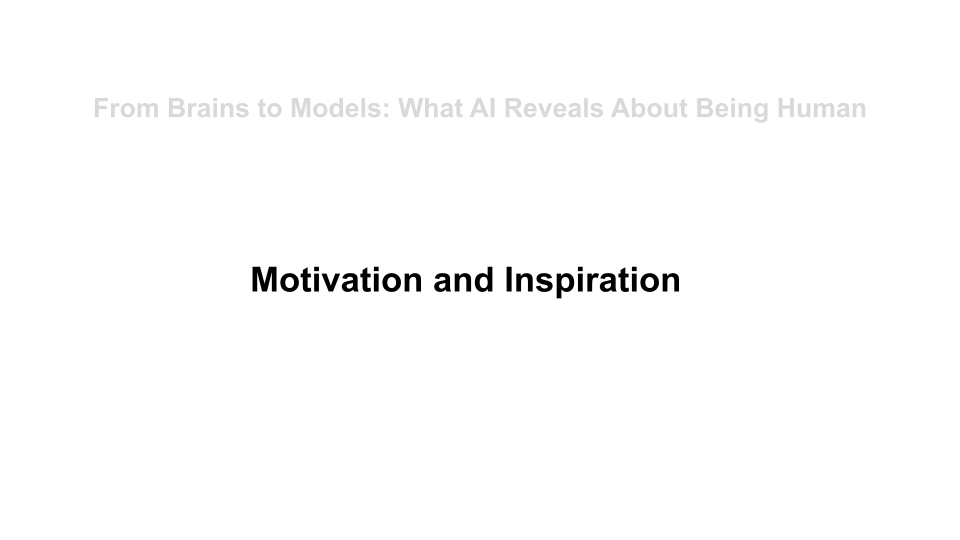
\includegraphics[width=.64\linewidth]{figures/talk/slide-02.png}}
\biopath
This divider invites you to identify a reason for learning the material. A useful starting question is: what would I need to understand before relying on an AI output in my own field? Choose an example such as identifying an enhancing lesion, following change over time, or explaining a positive screening result. List what is observed, what is inferred and what decision might follow. These are different stages, and each can fail in a different way. Image contrast can change with acquisition; a segmentation can inherit an annotation convention; an accurate probability can still leave a difficult choice.

The biomedical route begins with these meanings and then introduces the machinery needed to examine them. Predict a result before opening a notebook, inspect the result, and explain any surprise in ordinary language. For the screening example, try counting affected and unaffected people before using a formula. For the growth example, distinguish a simulated tissue state from the coloured boundary drawn around it. By the end, aim to give a colleague an explanation that includes the purpose, the evidence and one unresolved assumption. That is a stronger learning outcome than remembering a sequence of model names.
\comppath
Treat motivation as problem specification. An attractive implementation can quietly answer a different question from the one that motivated it. Write down an input, an output, an intended population and a criterion for success before choosing an architecture. Then identify the smallest runnable example that exposes the central issue. The course uses small systems because their assumptions can be inspected: fixed analytic classifiers, a trainable synthetic segmenter, an exact attention calculation, and reaction--diffusion simulations.

Distinguish three activities when using them. Demonstration shows that a phenomenon can occur under chosen conditions. Verification checks whether code implements the stated mathematics. Empirical validation asks whether the model describes observations sufficiently well for a specified purpose. A single notebook can support more than one activity, but the evidence for each must be identified separately. Start a learning log with a prediction and a possible failure criterion. After running, record the observed discrepancy and a proposed explanation. If a result agrees with your prediction, ask whether the test could have exposed a plausible bug or alternative mechanism. The computational route develops this habit alongside the calculations.
\end{slidenotes}

\begin{slidenotes}{03}{Biological brains across scales}{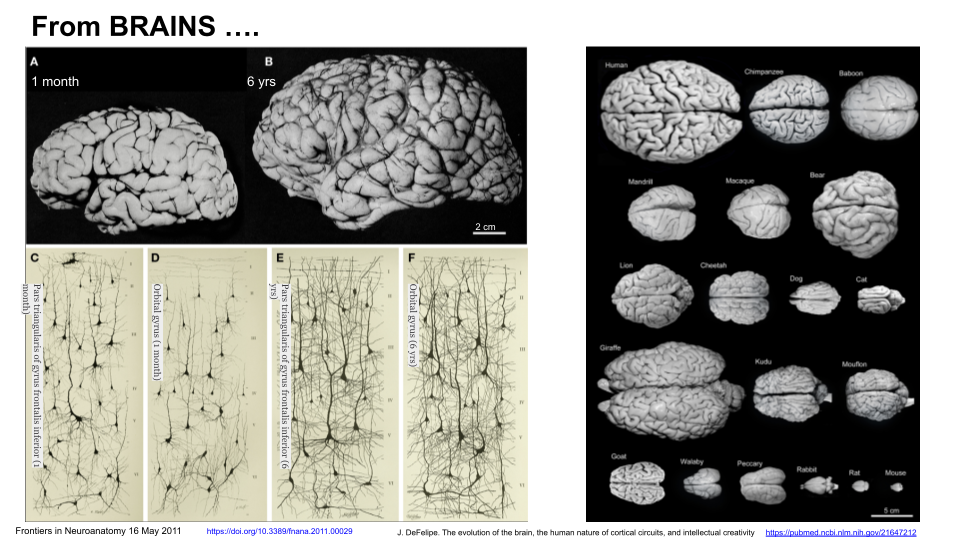
\includegraphics[width=.64\linewidth]{figures/talk/slide-03.png}}
\biopath
The slide juxtaposes cortical drawings at different developmental ages with brains from different mammals, drawing attention to biological diversity across scales. The neuron drawings concern local organisation; the whole-brain images concern macroscopic form. Their scale bars matter. A larger drawing on the page does not necessarily represent a larger biological structure. Nor does a difference in visible branching establish a difference in intelligence. Such claims would require appropriate measurements, comparable sampling and an account of development, species and behaviour.

For imaging students, this is a reminder that an MRI voxel aggregates signals from many microscopic components. A change in a macroscopic measurement may have several biological explanations. Conversely, a cellular change may occur without a detectable change in gross anatomy. Move carefully between scales: state which structure was observed, by which method, and which further process is being inferred. Brain development also includes interaction with a body and environment over time; a static anatomical panel captures only part of that history. As an exercise, choose one visible contrast in the slide and write a descriptive claim supported by the picture. Then write a mechanistic claim that would require additional data. Explain what those data would need to measure.
\comppath
The route from biology to computation begins with deciding which properties to model. A neuron can be represented by a detailed biophysical system, a firing-rate variable or a simple threshold unit, depending on the question. Each choice discards information. This is useful abstraction when the retained variables suffice for the target phenomenon; it becomes misleading when the omitted properties are needed to support the conclusion. The drawings therefore motivate a modelling decision rather than prescribe a particular artificial architecture.

Separate structural similarity from functional and causal similarity. Two networks could have comparable connection statistics yet compute different mappings. Two systems with different connectivity could produce similar answers on a restricted task. A convincing comparison needs a shared observable and a test that probes how it arises. For example, compare responses to the same controlled stimulus and then perturb a proposed pathway. \coursenotebook{03_bio_vs_artificial.ipynb}{Notebook 03} offers a supplementary comparison of learning systems; its architectures and learning rules change together, so an observed difference cannot be attributed to either factor alone. Design a hypothetical comparison that tests each learning rule in each architecture, so the two factors can be separated. This makes the limitations of an analogy informative rather than merely disappointing.
\end{slidenotes}

\begin{slidenotes}{04}{Architectures encode choices}{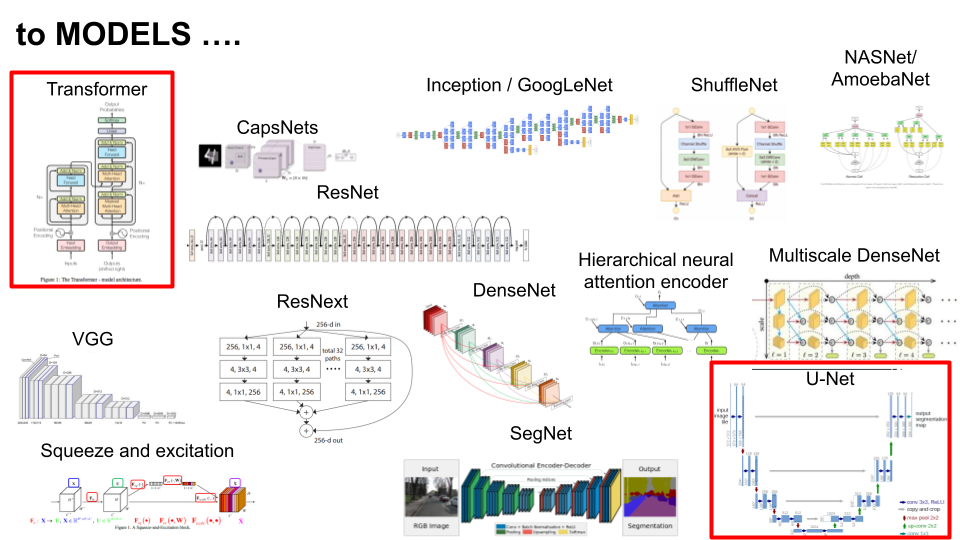
\includegraphics[width=.64\linewidth]{figures/talk/slide-04.png}}
\biopath
The architecture collage shows that there is no single design called ``the neural network''. Networks arrange computations in different ways to suit different tasks. A classifier may compress an entire image into a diagnosis-related score. A segmentation network must also preserve enough spatial information to assign labels to individual pixels or voxels. The highlighted U-Net family combines information at broader and finer spatial scales; the highlighted Transformer uses attention operations to combine information according to relationships within its input representation \citep{ronneberger2015,vaswani2017}.

For an imaging application, begin with the output needed and work backwards. Does the task require a local boundary, a whole-image category or a report? Which image contrasts and spatial relationships are available? A sophisticated architecture cannot restore information that was never measured, and a high average score can conceal failures on small lesions or unfamiliar acquisitions. Architecture names also say little about annotation policy, training population or calibration. Compare two candidate systems by asking what each sees, what it predicts, and how its errors would affect the intended use. The purpose of this slide is to recognise design choices and their implications; memorising every branch of the collage contributes much less to that judgment.
\comppath
An architecture specifies a family of functions and constrains how information flows. Convolutions reuse local filters; residual connections provide additive routes through a network; encoder--decoder structures combine spatial compression with reconstruction of an output grid. Attention computes input-dependent combinations of value vectors. These choices influence optimisation and the kinds of regularity that can be represented efficiently. Training then selects parameters within that family using a dataset, objective and optimisation procedure.

Do not infer an explanation from the diagram alone. A skip connection permits information flow, but demonstrating that a particular cue controls a prediction requires an intervention. Likewise, an attention matrix is one intermediate quantity rather than a complete account of the network's dependence on its input. Use \coursenotebook{01_tiny_transformer.ipynb}{Notebook 01} to trace a small Transformer and \coursenotebook{09_segmentation_reflection.ipynb}{Notebook 09} to inspect a trained synthetic segmentation example. Keep the output definition and evaluation examples fixed when comparing models. If several architectural and training choices change together, report the comparison as a comparison of systems. To attribute an improvement to a specific component, construct an ablation (a controlled removal or alteration of that component) and assess whether the conclusion survives relevant data shifts.
\end{slidenotes}

\begin{slidenotes}{05}{Four questions about intelligence}{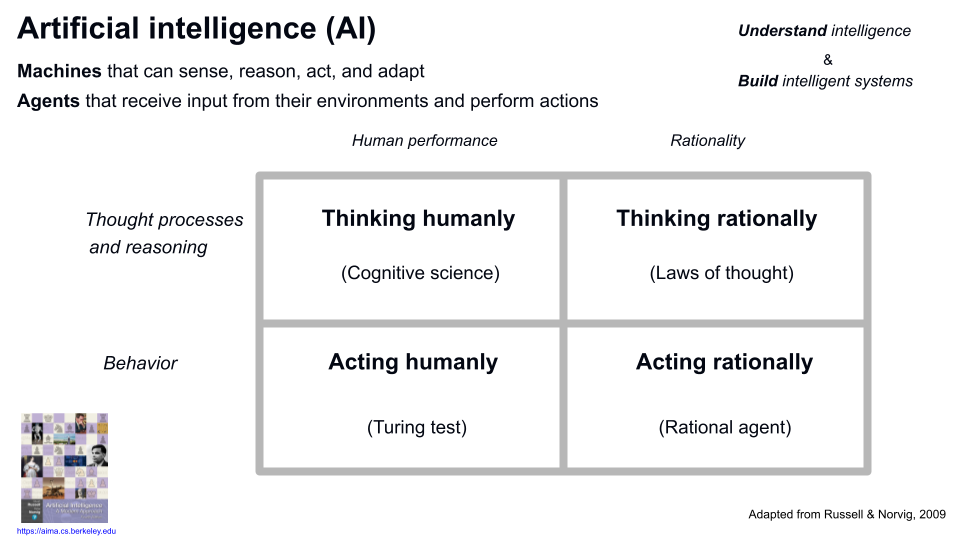
\includegraphics[width=.64\linewidth]{figures/talk/slide-05.png}}
\biopath
The Russell--Norvig grid crosses two distinctions: thinking versus acting, and human resemblance versus rational performance. Each cell asks a different question. A system can reproduce a clinician's answers, model the clinician's reasoning process, make formally consistent inferences, or select actions that serve a specified objective. These achievements can come apart. Matching a historical prescribing pattern, for example, could reproduce a systematic mistake. Following a formal rule could also be inappropriate if the rule omits an important patient concern.

Use the grid to clarify what an evaluation establishes. Agreement with an expert measures a form of behavioural resemblance. A study of response times or error patterns can contribute evidence about processing. Expected-utility analysis evaluates actions relative to stated outcomes, probabilities and preferences. Calling an action rational does not make those preferences universal or remove uncertainty. In clinical work, ask who defined the objective and whose outcomes were counted. Take a familiar diagnostic decision and place four possible research questions into the four cells. Then choose the evidence each would require. The same AI system may be relevant to all four questions, but a successful test in one cell does not answer the others.
\comppath
Translate each cell into an observable target. ``Acting humanly'' could mean that a judge cannot reliably distinguish a model's answers from human answers under a fixed protocol. ``Thinking humanly'' needs a model of process and predictions that discriminate it from alternatives. ``Thinking rationally'' might concern valid inference within a specified formal system. ``Acting rationally'' concerns action selection relative to an objective and available information. The labels become useful only when the task and success criterion are explicit.

\coursenotebook{04b_four_views_of_AI.ipynb}{Notebook 04b} treats the grid as a catalogue of evaluation questions. It does not supply a measured verdict on a named model. Use it to identify a common category error: optimising agreement with human labels and then claiming optimal decisions. A classifier trained to minimise prediction loss does not automatically minimise the downstream cost of acting. Conversely, a decision policy can be useful while producing explanations unlike human reasoning. For an exercise, define separate metrics for human agreement and expected decision cost on the same constructed cases. Work out a case in which the metrics rank two systems differently. The disagreement identifies the extra assumptions needed to choose between them.
\end{slidenotes}

\begin{slidenotes}{06}{Embodiment, judgment and collaboration}{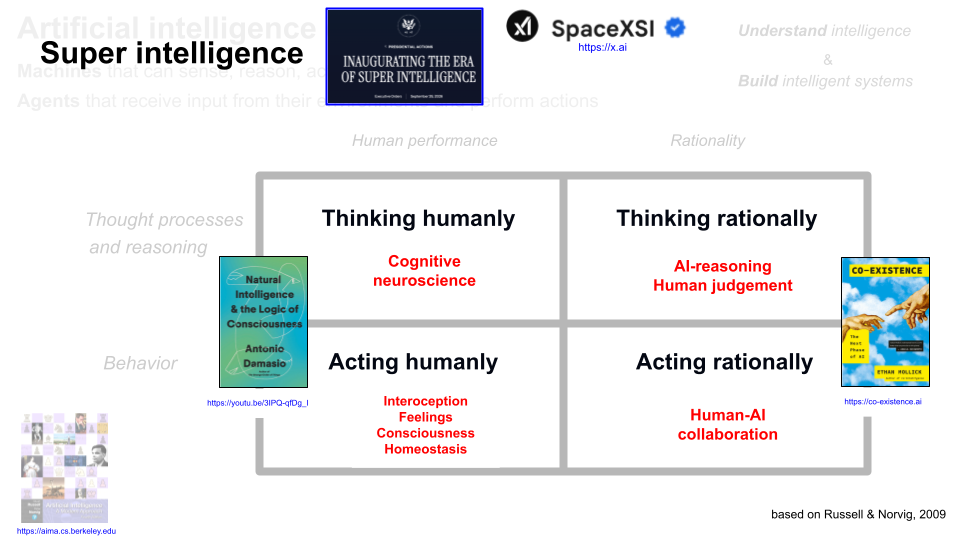
\includegraphics[width=.64\linewidth]{figures/talk/slide-06.png}}
\biopath
The annotated grid extends the previous slide towards cognitive neuroscience, judgment, feelings and collaboration. Interoception concerns signals about the body's internal condition; homeostasis concerns regulation that keeps physiological variables within viable ranges. These processes help explain why biological cognition is bound to needs, action and a continuing life. Their presence in the discussion motivates questions about embodied understanding. It does not supply a simple anatomical test for consciousness or a proof that one particular mechanism is sufficient for experience \citep{seth2013,sethbayne2022}.

In medicine, collaboration can be evaluated even when these philosophical questions remain open. Consider an AI-drafted explanation of a scan. Its wording may be fluent while the clinician must still recognise uncertainty, respond to distress and connect the explanation to the patient's circumstances. Assess the combined interaction: what information was conveyed, what the patient understood, and what responsibility the professional exercised. The books and headlines on the slide are prompts for discussion rather than experimental evidence. Choose one claim, such as ``this system understands the patient's concern'', and specify a narrower observation that could be tested. Then identify what would remain uncertain even if that observation were positive.
\comppath
A regulated software system can monitor variables, maintain constraints and pursue goals. These functional properties are worth describing precisely. They do not by themselves settle whether its states have the biological or experiential significance of hunger, pain or concern. Keep functional terms tied to an operation: a controller reduces an error signal; an agent selects tool calls; a language model produces a context-dependent continuation. Moving from an operation to a claim about subjective experience requires a further argument and evidence.

Human--AI collaboration introduces another unit of analysis: the coupled system of model, interface, professional and environment. Measure whether assistance improves performance under the actual division of labour. Useful comparisons include unaided judgment, unaided model output and the combined workflow, with the same cases and outcome definition. Examine whether assistance changes error detection or encourages inappropriate agreement. Appendix~\ref{app:4e} develops embodied, embedded, enactive and extended perspectives as questions that can guide such studies. As a computational exercise, describe a feedback loop and identify the state variables that belong to the software, the user and the environment. This makes the brain analogy specific enough to investigate without allowing the analogy to stand in for evidence.
\end{slidenotes}

\begin{slidenotes}{07}{What a Turing-like test measures}{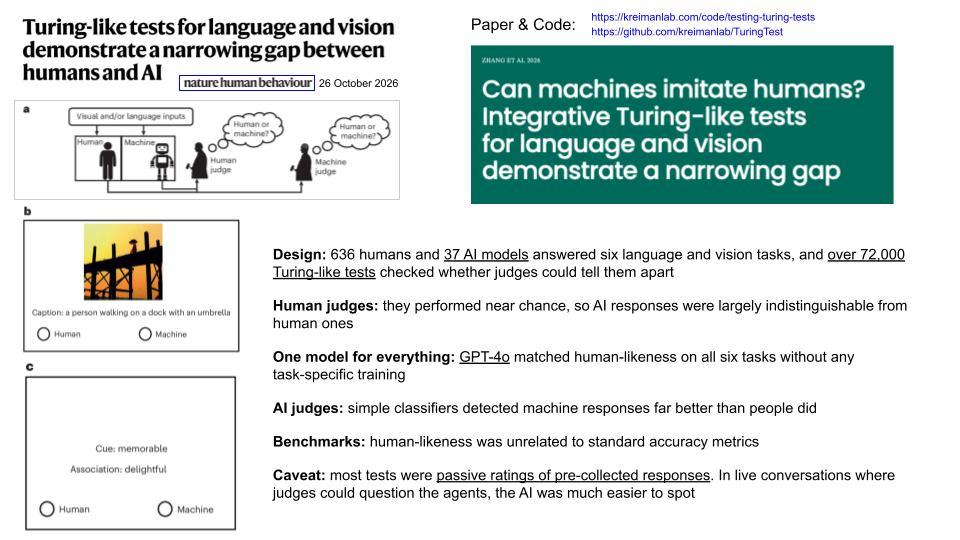
\includegraphics[width=.64\linewidth]{figures/talk/slide-07.png}}
\biopath
The displayed study examines whether judges can distinguish human from machine responses on specified language and vision tasks. It is a test of detectable human resemblance under a protocol. In the published version, 636 human contributors and 37 AI models supplied responses; 72,191 refers to judgment trials, not independent participants. Near-chance discrimination in some conditions does not imply that all models passed every task \citep{zhang2026turing}.

An everyday clinical analogy helps separate the questions. A machine-written report may sound convincingly human while containing an incorrect measurement. A terse, recognisably automated output may contain the correct measurement. Humanness, accuracy and usefulness therefore need separate assessments. A judge may also rely on a superficial cue, such as habitual wording, rather than the quality of the reasoning. Suppose an apparently human report contains a subtle contradiction between the findings and conclusion. What would a source-identification test reveal, and what would a clinical review reveal? Use the distinction to design two evaluation forms: one asks who produced the report; the other checks its factual and interpretive content. Neither should be used as a substitute for the other. The slide invites an operational question about behaviour, while leaving mechanisms and experience open.
\comppath
Treat source identification as a classification problem. Specify the sampling of human and model answers, information available to the judge, class balance and metric. Fifty per cent accuracy is a chance reference for a balanced binary task, but a confusion matrix reveals whether the judge systematically favours one source. Repeated judgments about the same answer are dependent observations; uncertainty estimates should respect the sampling structure rather than count every click as a new independent response.

Separate answer quality from detectability by measuring both on the same items. A model could become harder to identify by reproducing human mistakes, so improved imitation need not indicate improved task performance. Similarly, a detector can exploit a collection artefact that disappears in a new setting. Hold out stimuli or participants as appropriate and ask whether source-specific preprocessing creates unintended cues. The authors also evaluate AI judges; comparisons require attention to differences in training and task conditions. For a small exercise, create responses with an irrelevant formatting cue correlated with source. Compare a detector before and after the cue is removed. A large performance drop would diagnose a property of the benchmark construction rather than a general ability to recognise machine reasoning.
\end{slidenotes}

\begin{slidenotes}{08}{Read results in their time and protocol}{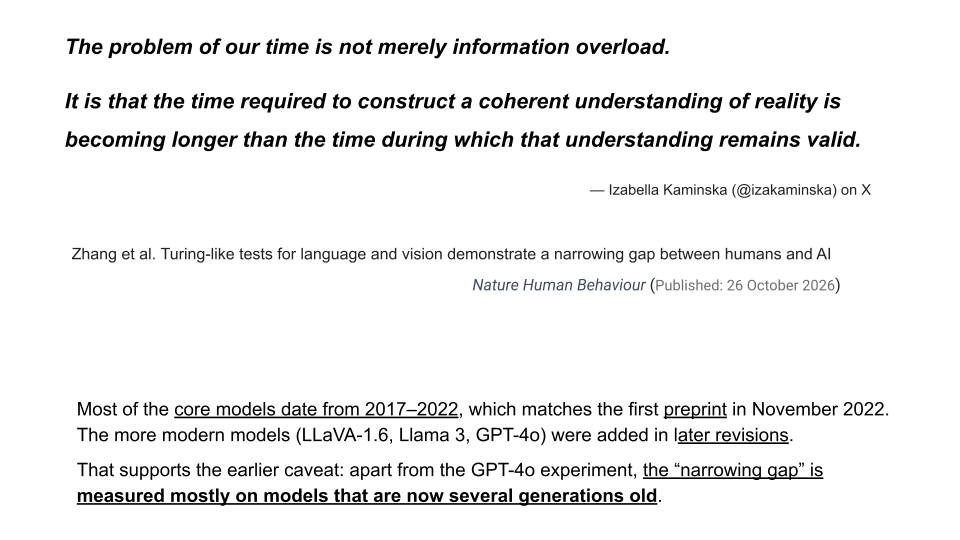
\includegraphics[width=.64\linewidth]{figures/talk/slide-08.png}}
\biopath
The quotation on the slide encourages scrutiny of a study's continuing relevance. A publication date and a model's release date answer different questions: when evidence appeared and which system was tested. Findings about an older system remain evidence about that system and setting. Applying them to a newer tool requires an additional comparison. The published Turing-like study also includes Claude 3.7 and LLaMA 3.3 conversation experiments, so the thumbnail's emphasis on older models is incomplete \citep{zhang2026turing}.

For clinical readers, think of a diagnostic assay that changes between study and deployment. Evidence is neither automatically obsolete nor automatically transferable. Identify what changed: the instrument, instructions, sampled population or outcome definition. An updated language model could improve factual responses while becoming easier to recognise, or the reverse. The original study can still offer a useful protocol, error taxonomy or comparison baseline. Write a short appraisal with three sentences: what was actually measured, which features of your intended use match that setting, and which difference requires new evidence. This practice avoids turning a debate about the age of technology into a vague verdict on an entire paper. It also makes a replication question sufficiently precise to answer.
\comppath
Version is part of the experimental specification. Record the model identifier, access date, system instructions, generation settings and input preprocessing alongside the evaluation code. A name that refers to a changing service is weaker provenance than a fixed snapshot. Where exact replay is unavailable, save permissible inputs and outputs and describe the limits of repeatability. These records allow a later researcher to separate a changed system from a changed measurement procedure.

The published study distinguishes passive assessment of existing responses from interactive questioning. Those protocols provide different information to a judge; changes in models and instructions also prevent treating every difference as an isolated effect of interactivity. To investigate one factor, hold the others fixed where possible. A useful replication matrix crosses model version with protocol, using matched tasks and explicit human sampling. Predefine the source-identification metric and a separate task-quality score. Do not tune the prompt on the final evaluation items. Finally, state whether the replication tests a historical result, an updated capability or transfer to a clinical task. Each objective supports a useful experiment, but combining them without a design makes a changed score difficult to interpret.
\end{slidenotes}

\begin{slidenotes}{09}{Turn a model suggestion into a study}{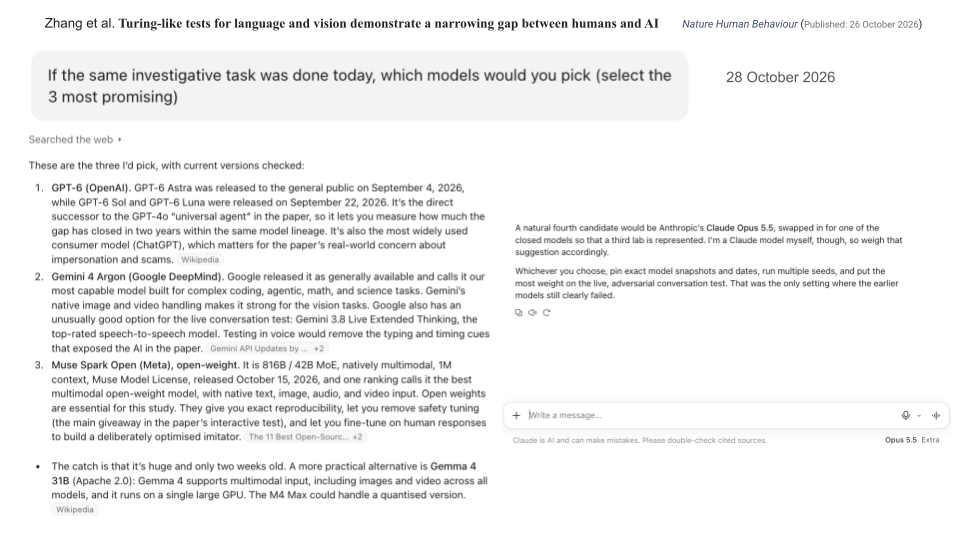
\includegraphics[width=.64\linewidth]{figures/talk/slide-09.png}}
\biopath
This slide shows an AI-generated proposal for choosing contemporary models to revisit the preceding study. Read it as a draft research suggestion. A confident list of names and capabilities is not a completed comparison, and the screenshot supplies no performance evidence for the proposed systems. The first educational task is to turn the suggestion into a question: are we testing human resemblance, answer accuracy, or suitability for a particular clinical activity?

Choose a clinically intelligible task before choosing a favourite model. For example, ask whether a short explanation preserves uncertainty and agrees with a supplied imaging report. Define what a human comparison group receives and what the judges are allowed to inspect. Include experts when factual adequacy requires domain knowledge; a general reader can judge clarity but may miss a subtle diagnostic error. Decide in advance what would count as improvement and what kind of error would be unacceptable for the proposed use. A small pilot can expose ambiguous instructions, but pilot cases should not silently become the final test set. The value of the suggestion is therefore its capacity to initiate a disciplined comparison. Its persuasive presentation should not determine the conclusion.
\comppath
Convert the screenshot into a reproducible protocol. First verify that each candidate system exists, is accessible and supports the required input modality at the time of the experiment. Record exact versions and settings instead of treating the proposed list as a current recommendation. Next define shared inputs, allowed tools, response limits, parsing rules and handling of failed or incomplete outputs. Differences in tool access or context can otherwise masquerade as differences between base models.

Separate protocol development from evaluation. Use development items to resolve formatting and instructions, then freeze the procedure before testing held-out stimuli. Repeated runs estimate variability under the chosen generation settings; report that variability alongside the human sampling uncertainty. Inspect whether multiple judgments or outputs share the same underlying item, and analyse the corresponding dependence. Include a straightforward baseline so that elaborate prompting must justify its added complexity. Save a failure log with examples and explanations that can be checked independently. Finally, distinguish a prospective design from measured results in every table and caption. This exercise illustrates a productive use of AI in research: generating a candidate plan whose assumptions, feasibility and conclusions are then examined by the investigator.
\end{slidenotes}

\begin{slidenotes}{10}{From patient data to a useful decision}{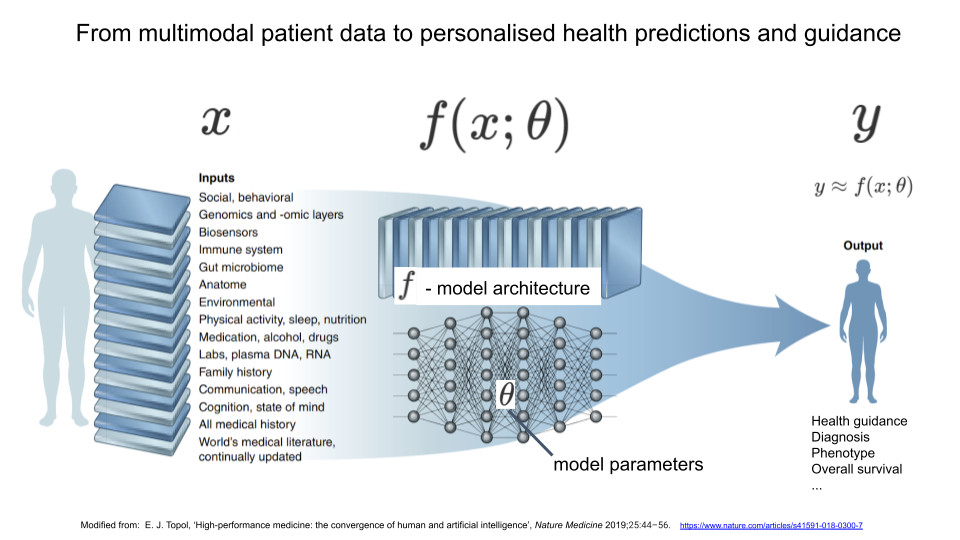
\includegraphics[width=.64\linewidth]{figures/talk/slide-10.png}}
\biopath
The diagram brings together measurements such as images, molecular data and clinical information as inputs to a model, which produces an output relevant to care. The notation $x\mapsto f(x;\theta)\mapsto y$ compresses a long chain. Someone decides what to measure, aligns records, defines an outcome and chooses how a predicted quantity enters practice. A probability of progression, an anatomical label and a treatment recommendation have different meanings and require different evidence.

Consider predicting an outcome at the time of a scan. Only information available then belongs in the intended prediction setting. A later investigation or a note written after the outcome can make retrospective accuracy look impressive while being unavailable when needed. Missing measurements can also carry information about referral and clinical practice rather than disease alone. Ask when each input was obtained and why it exists. Then distinguish prediction from action: an estimated risk does not specify how a patient values treatment burdens. Section~\ref{sec:decisions} and \coursenotebook{15_ppv_and_decisions.ipynb}{Notebook 15} show why prevalence and stipulated consequences matter. A useful explanation of this diagram should therefore connect the patient, measurement process, predicted quantity and decision, rather than stop at the central model box.
\comppath
Here $x$ denotes the input representation, $\theta$ the fitted parameters and $y$ the target or predicted output, depending on the diagram's convention. Make that last distinction explicit in implementation: a reference outcome and an estimate of it are separate objects. Multimodal learning also requires an alignment rule. Images, laboratory results and notes must refer to the appropriate person and time; otherwise the apparent benefit of combining modalities can arise from leakage or mismatched sampling.

Evaluate the full pipeline, including preprocessing and missing-data handling, using patient-level separation where patients contribute repeated records. A held-out hospital or later time period can probe transfer beyond the development setting. Assess calibration when predicted probabilities will support decisions, and measure clinically relevant error patterns as well as aggregate discrimination. A model estimating outcomes under observed care does not automatically estimate the effect of changing treatment: treatment selection and confounding enter that causal question. \coursenotebook{11_shortcut_dependence.ipynb}{Notebook 11} provides a controlled illustration of reliance on constructed cues using fixed analytic rules. Use it to formulate an intervention on an irrelevant input feature before claiming that a multimodal representation has learned the intended biological relationship.
\end{slidenotes}

\begin{slidenotes}{11}{Keep the task fixed across Marr's levels}{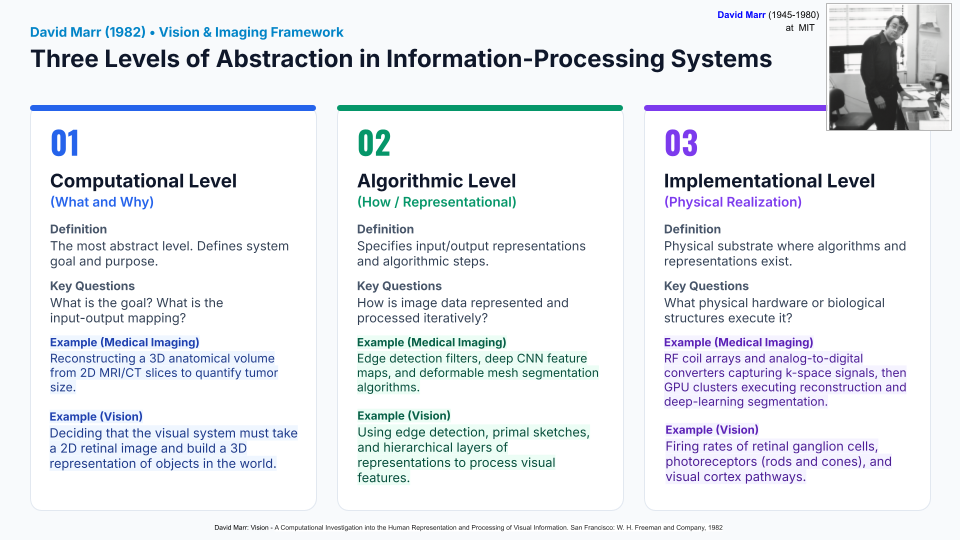
\includegraphics[width=.64\linewidth]{figures/talk/slide-11.png}}
\biopath
Marr separates an explanation of what a system does and why, an account of its representations and algorithms, and its physical implementation \citep{marr2010}. Keep one task fixed to see the distinction. Suppose the aim is to compare the spatial extent of enhancing tissue across two examinations. At the computational level, define that target and explain why measuring it is useful. At the algorithmic level, describe how an image becomes a mask and how the mask becomes a volume. At the implementation level, identify the hardware that stores the data and executes those operations.

A simple volume calculation makes this tangible. If a mask contains 1,000 voxels and each voxel occupies 2~mm$^3$, the represented volume is 2,000~mm$^3$, or 2~mL. This calculation can be exact even when the mask boundary is uncertain or enhancement is an imperfect marker of the biological quantity of interest. The slide ranges across acquisition, reconstruction and segmentation; in discussion, avoid switching among them unnoticed. MRI reconstruction estimates an image from acquired signals, while segmentation assigns labels to an image. Choose one of these tasks before filling in the three columns. The framework then helps locate a disagreement rather than merely rename it.
\comppath
For the fixed lesion-volume task, specify the input image and target convention first. A possible representation is a binary array $m_i\in\{0,1\}$ with voxel volumes $v_i$; an algorithm computes $V=\sum_i m_iv_i$. The mask itself may come from manual annotation, a convolutional network or another procedure. Those alternatives share a downstream calculation while differing in how they obtain its inputs. The physical realisation includes memory, processors and numeric representations used to execute the chosen procedure.

Different levels constrain one another without being interchangeable. Available memory can restrict image resolution, which can affect the accuracy of a boundary estimate. Yet identifying a GPU does not establish that the segmentation policy is appropriate. Likewise, agreeing on the clinical purpose does not specify a correct algorithm. In MRI, radiofrequency signals are sampled in a measurement domain often described through k-space; a stack of reconstructed slices is already a processed representation. Keep these stages distinct when describing the implementation examples on the slide. \coursenotebook{00_intro_timeline.ipynb}{Notebook 00} offers a starting exercise. For a proposed improvement, identify which level changes and which observation would demonstrate its benefit. Explicit clinical context accompanies all three levels; it is not a fourth level in Marr's original framework.
\end{slidenotes}

\begin{slidenotes}{12}{Read about AI with an application in mind}{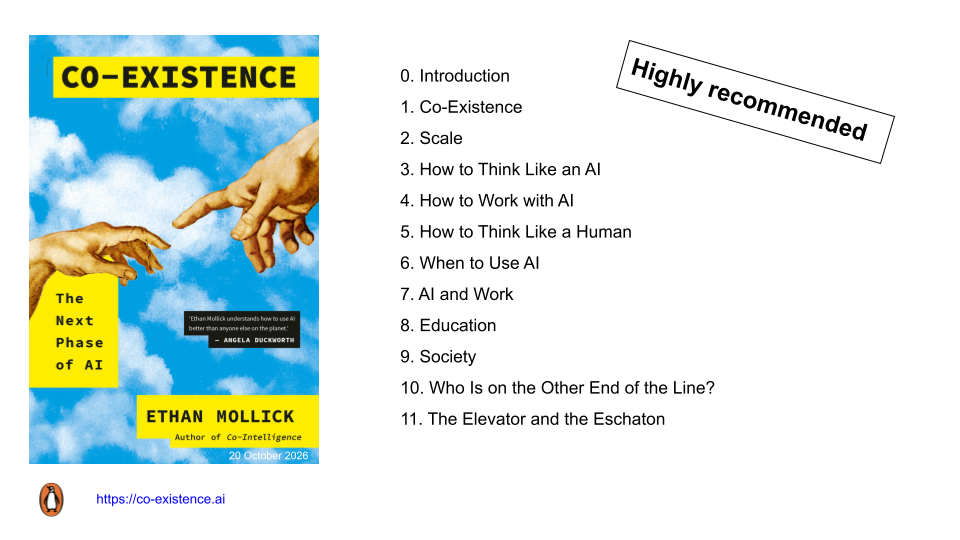
\includegraphics[width=.64\linewidth]{figures/talk/slide-12.png}}
\biopath
The book recommendation marks a move from comparing systems to learning how to work with them. Mollick's \emph{Co-Existence} spans AI capabilities, human thinking, work, education and society \citep{mollick2026coexistence}. Use that breadth to generate questions relevant to your own practice. A chapter about education, for example, can prompt a distinction between completing an assignment and acquiring the ability to solve the next problem unaided. A chapter about work can prompt an examination of how verification effort changes when drafting becomes easier.

Read actively rather than treating a recommendation as a settled account of every domain. Select one claim, identify the setting in which it might apply, and ask what evidence would support transfer to biomedical work. A tool that helps brainstorm a patient-information leaflet still needs checking for factual accuracy, audience understanding and suitability for the situation. Keep a short reading note with a claim, a concrete example and a testable implication. Then compare your interpretation with someone taking the other path. The aim is to connect a broad account of technological change to a carefully bounded learning or research task. The book is a discussion resource; the particular application supplies the evaluation question.
\comppath
Use the table of contents as a map of levels at which an AI system can be studied: model behaviour, user interaction, organisational workflow and social consequences. A performance benchmark concerns a different unit of analysis from a study of whether a team becomes more effective. The same underlying model can support very different outcomes depending on the interface, instructions, checks and division of labour. Define that surrounding system before comparing productivity claims.

For a small study, choose a task with a checkable output, such as extracting a fixed set of fields from supplied reports. Measure accuracy, completion time and review time separately. Record corrections and unresolved cases rather than counting every generated field as completed work. If the goal is learning, add a later unaided task; if the goal is workflow improvement, include the cost of detecting errors. These choices allow a clear comparison between immediate output and retained competence. Make explicit which parts of the procedure come from your own design and which are hypotheses inspired by the reading. A general book can help formulate useful questions, while a reproducible protocol determines what your experiment can establish about a specific tool and context.
\end{slidenotes}

\begin{slidenotes}{13}{Preserve the ability to judge}{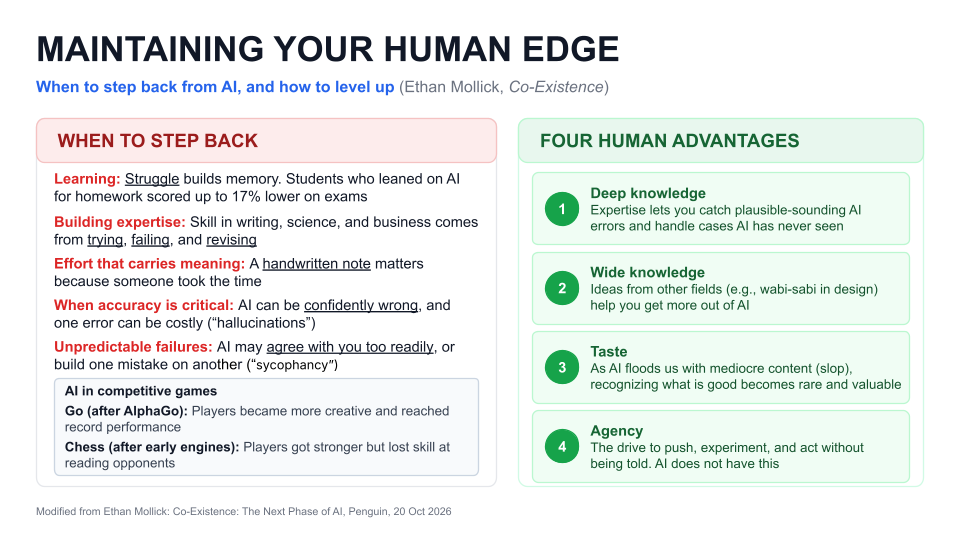
\includegraphics[width=.64\linewidth]{figures/talk/slide-13.png}}
\biopath
The slide asks when assistance strengthens your work and when it removes the practice needed to become competent. Its examination statistic refers to a particular high-school mathematics experiment: the unrestricted GPT-4 group scored 17\% lower than the control group when assistance was removed; a tutor designed with learning safeguards largely mitigated that effect \citep{bastani2025learning}. This is not a universal effect size for AI use, university students or medical education. It illustrates why assisted performance and subsequent independent learning should be measured separately.

Hallucination is plausible but unsupported content; sycophancy is inappropriate agreement with the user. In imaging education, try describing a scan or checking a volume calculation yourself before viewing an AI answer. Then compare the explanations, identify the discrepancy and solve a related case without assistance. Asking for a hint can preserve more of this work than requesting a finished answer. The slide's proposed human strengths---depth, breadth, taste and agency---can be translated into practice: know enough to detect an error, connect ideas across fields, justify a quality judgment and take responsibility for a choice. Treat its game-playing examples as discussion prompts rather than evidence of a general educational law. The central question is whether a particular pattern of tool use develops or bypasses the competence you are trying to acquire.
\comppath
When studying assistance, choose outcomes that distinguish output production from skill acquisition. Immediate accuracy, review accuracy and delayed unaided transfer are different variables. A learner can complete more tasks with a tool while becoming less able to diagnose a new failure independently. Randomised assistance conditions and common unaided assessments can help identify that distinction. Preserve the task difficulty and scoring rule across groups, and account for the possibility that users respond differently to direct answers and guided hints.

The slide's statement about agency also needs a precise reading. Software agents can select actions and pursue assigned objectives; this is a functional property that can be implemented and tested. The broader claim concerns self-originated human motivation, meaningful commitments and responsibility, which are not established merely by observing a sequence of tool calls. Describe the operational capability before drawing a philosophical conclusion. As an exercise, inspect an AI-produced solution that contains one subtle unit error. Record whether you can find and explain it before running a checker. Then design assistance that supports diagnosis without immediately revealing the correction. A useful learning system should make the student's reasoning more inspectable and transferable, not only increase the number of plausible answers on the page.
\end{slidenotes}

\begin{slidenotes}{14}{Map the frontier task by task}{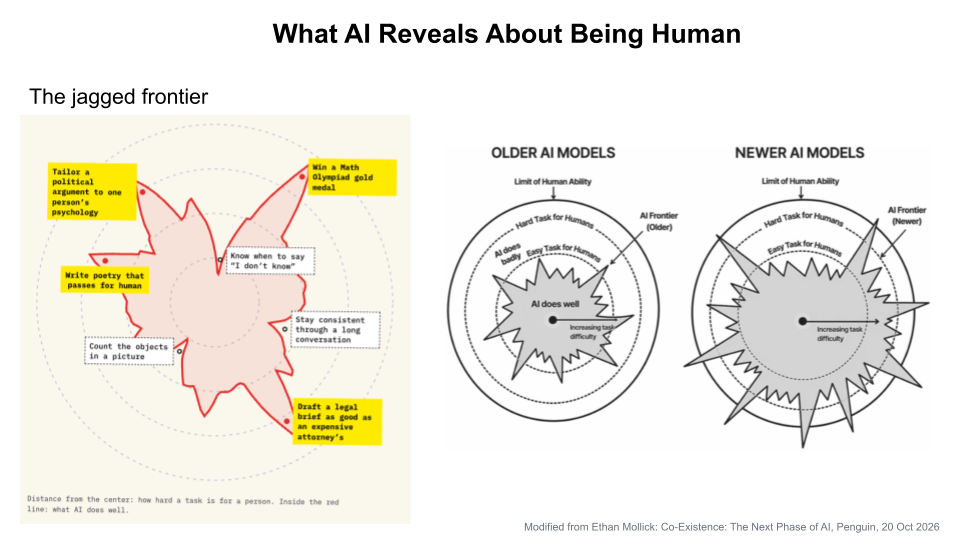
\includegraphics[width=.64\linewidth]{figures/talk/slide-14.png}}
\biopath
The jagged boundary represents uneven capability: a system may perform well on a task people find difficult yet fail on a task people find easy. The diagrams are conceptual illustrations, not measured maps of a clinical tool \citep{mollick2026coexistence}. Their radial arrangement should not be read as a calibrated scale of intelligence. The useful message is that intuition about human difficulty offers an unreliable guide to the reliability of an unfamiliar AI system.

Apply this to an imaging workflow. A model might produce a fluent summary yet mishandle a small numerical comparison, laterality or the timing of an examination. Conversely, it might identify a subtle image pattern consistently while failing to explain its significance. These are candidate failure modes to test, not conclusions supplied by the diagram. Break the workflow into observable operations and evaluate each on representative cases. Include uncommon but consequential situations rather than relying entirely on average performance. If a system changes, repeat the relevant checks instead of assuming that every capability improves together. The practical exercise is to draw your own evidence map: put a task, its observed errors and its tested conditions beside each point. Leave untested territory explicitly unmeasured.
\comppath
A capability frontier depends on model version, prompting, tool access, data distribution and the chosen success threshold. It is therefore a property of an evaluation setting as well as a model. Replace the sketch with a table of tasks and measurable criteria. For each task, report the number and source of examples, the metric, uncertainty and observed failure modes. A boundary inferred from a handful of demonstrations is likely to move when the input distribution changes.

Avoid selecting only examples that confirm a preferred picture. Use a development set to formulate the task categories and an independent test set to estimate performance. If an agent can retry or use tools, include those resources in the protocol and cost comparison. Compare the same tasks across system versions rather than comparing different benchmark collections. A regression on one operation can matter even when an aggregate score rises. \coursenotebook{11_shortcut_dependence.ipynb}{Notebook 11} supplies a small example of how changing a cue relationship can alter the ranking of fixed classifiers. Use it to explain why capability under one distribution does not establish robustness under another. The operational counterpart of the jagged sketch is a maintained set of relevant tests, including the failures that motivated them.
\end{slidenotes}

\begin{slidenotes}{15}{Specify, inspect, revise and stop deliberately}{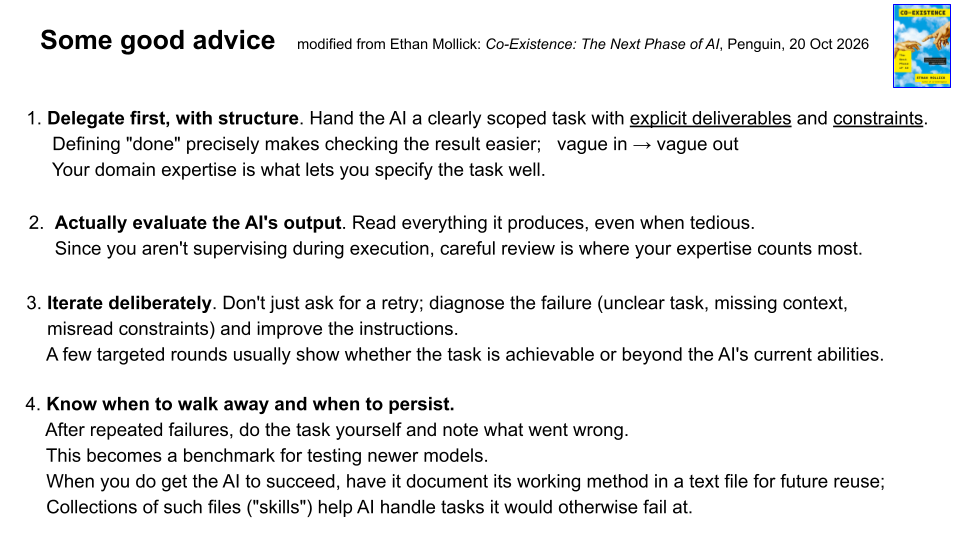
\includegraphics[width=.64\linewidth]{figures/talk/slide-15.png}}
\biopath
The four recommendations turn collaboration into a sequence you can inspect: define a bounded task, examine the result, diagnose the failure and decide whether further work is worthwhile. Consider asking for an explanation of a segmentation result. Specify the intended audience, the supplied evidence and the distinction between an image finding and a biological interpretation. A useful deliverable might be a short explanation that preserves uncertainty and defines the unfamiliar terms. You can then assess whether the result meets those requirements.

Evaluation must include the content that a polished answer makes easy to overlook. Check numbers against the source, follow citations to the actual passage, and ask whether the conclusion goes beyond the observations. If a term was misunderstood, revise that part of the instructions and retain the failed example for comparison. Repeated confident errors suggest that more prompting may be less useful than doing the task directly or consulting an appropriate source. When a procedure works, document the inputs and checks that made it work. A reusable method should help the next user recognise a failure as well as reproduce a success. This is a practical interpretation of the advice on the slide, adapted to accountable biomedical work.
\comppath
Express the task as an input--output contract with acceptance criteria. For a simulation request, specify the equation, units, boundary conditions, parameters and outputs before requesting code. Then use independent checks: a spatially uniform solution, a conservation property or a comparison with a trusted limiting case. Successful execution and attractive plots are weak evidence if no test could distinguish the intended model from a plausible incorrect implementation. \coursenotebook{13_verified_growth_model.ipynb}{Notebook 13} demonstrates several stronger checks.

Iteration should be diagnostic. Preserve the failing input, error and expected behaviour; change the suspected cause; then rerun the relevant check. Changing many instructions simultaneously can repair an output while obscuring what was wrong. A model-generated explanation of its own success is a hypothesis to investigate, not an independent verification. Define a stopping rule in terms of unresolved errors, available evidence and the cost of further attempts. Save a working method with its environment, dependencies and known limits so that another person can use it. This makes the slide's practical advice testable and supports a useful division of labour: AI can propose and implement, while acceptance rests on explicit criteria and evidence that can be examined outside the generation process.
\end{slidenotes}

\begin{slidenotes}{16}{Compartments, anatomy and measurement}{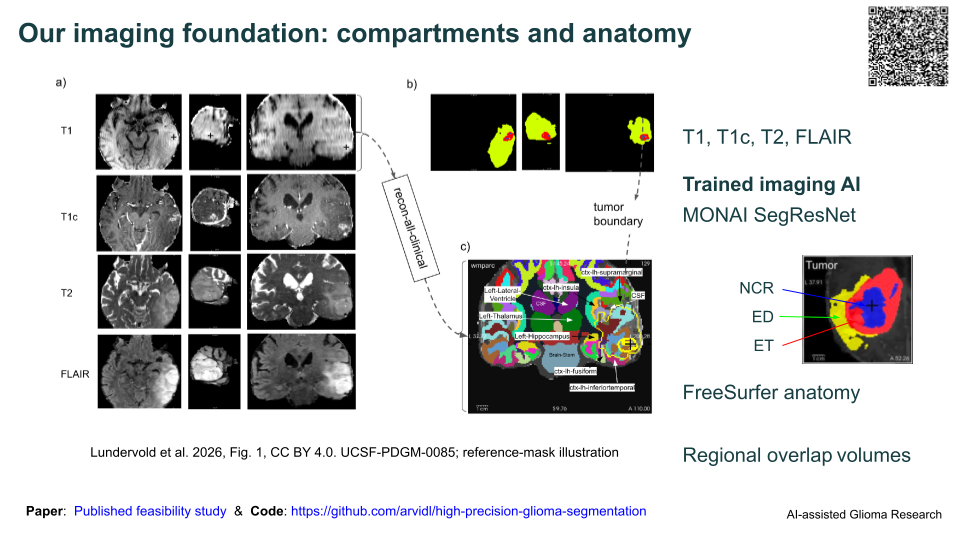
\includegraphics[width=.64\linewidth]{figures/talk/slide-16.png}}
\biopath
The multiparametric MRI panel combines T1-weighted images, contrast-enhanced T1 (T1c), T2-weighted images and fluid-attenuated inversion recovery (FLAIR). T1c emphasises contrast enhancement; T2 and FLAIR reveal different water-related signal changes, with FLAIR suppressing cerebrospinal-fluid signal. In the displayed compartment convention, NCR denotes a necrotic/non-enhancing core category, ED an oedema-related region, and ET enhancing tumour. They are imaging label categories; their boundaries are not direct microscopic maps of every viable tumour cell. Enhancement and surrounding signal changes require interpretation in their clinical context.

The slide links those compartments to anatomical regions obtained with FreeSurfer, enabling overlap volumes. For example, the amount of a labelled lesion region inside an anatomical parcel answers a spatial measurement question. It does not alone establish functional impairment or identify infiltrating cells beyond the visible abnormality. The displayed compartment panel uses reference masks from the published feasibility study, credited in the thumbnail; it should not be read as a newly computed SegResNet prediction \citep{lundervold2026glioma}. When discussing a volume, name the compartment, anatomical coordinate system and annotation convention. Ask how partial volume, registration errors or a different labelling policy could alter the number. This connects a visually convincing overlay to the practical work required for a defensible measurement.
\comppath
Trace two outputs that are combined in the figure: a tumour-compartment segmentation and an anatomical parcellation. An overlap calculation requires both to occupy the same physical coordinate frame. Matching array dimensions is insufficient; orientation, voxel spacing and image-to-world transforms matter. For masks $m_i$ and $a_i$ on a common grid, the intersection volume is $\sum_i \mathbf{1}[m_i=1\land a_i=1]v_i$. Resampling labels generally requires a method that preserves discrete categories rather than inventing intermediate class values.

Evaluate the segmentations and the derived measurements separately. A modest boundary discrepancy can matter substantially for a small compartment or a regional overlap. Also distinguish a reference annotation from biological ground truth: agreement measures consistency with the reference policy. The slide identifies MONAI SegResNet as trained imaging AI, while \coursenotebook{09_segmentation_reflection.ipynb}{Notebook 09} is a separate synthetic exercise with a tiny NumPy model. Its controlled labels and interventions support teaching about dependence and policy; they do not reproduce the research system's patient results. For an exercise, translate one mask by a voxel and recompute regional overlap. Compare how much the total compartment volume and the intersection change. The difference demonstrates why registration quality belongs in the measurement pipeline.
\end{slidenotes}

\begin{slidenotes}{17}{Population growth and a mechanistic hypothesis}{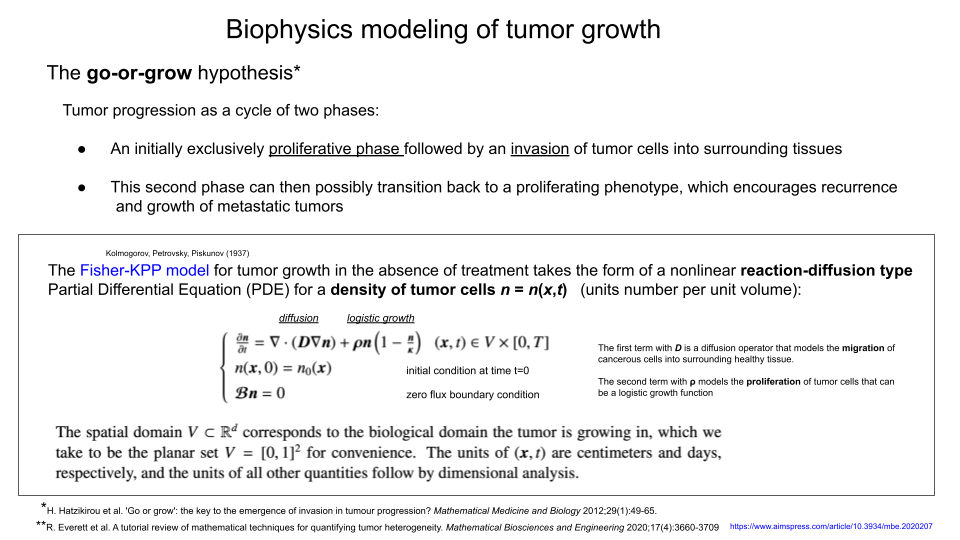
\includegraphics[width=.64\linewidth]{figures/talk/slide-17.png}}
\biopath
The equation combines spatial dispersal with local growth. A cell-density field says how many cells are represented per unit volume at each location. The dispersal term smooths density differences, while logistic growth slows as density approaches a chosen carrying capacity. These are population-level approximations. They can illustrate an advancing infiltrative pattern without tracing individual cells or resolving blood vessels and tissue microstructure.

The go-or-grow hypothesis concerns a possible trade-off between migration and proliferation, potentially involving changing cellular states \citep{hatzikirou2012}. The slide's wording about two phases should not be read as a compulsory, globally synchronised sequence. The displayed Fisher--KPP equation has one density variable and includes dispersal and growth simultaneously; it contains no explicit phenotype switching. Its mention of metastatic growth is also broader than the intended local glioma-invasion example. Keep the biological hypothesis distinct from what the equation actually implements. In \coursenotebook{14a_growth_density_and_thresholds.ipynb}{Notebook 14a}, change a display threshold while leaving the simulated state fixed. The visible boundary moves even though the underlying density does not. This is an important bridge to imaging: a thresholded outline is an observation convention, whereas a mechanistic claim concerns the process generating the state.
\comppath
Write the model as $\partial_t c=\nabla\!\cdot(D\nabla c)+\rho c(1-c/K)$, with initial density $c(\mathbf{x},0)=c_0(\mathbf{x})$ and a zero-flux boundary. If distance is measured in millimetres and time in days, $D$ has units mm$^2$/day, $\rho$ has units day$^{-1}$, and $c$ and $K$ share density units. Every term then has units of density per day. The slide's spatial-unit convention differs from the local notebooks; numerical parameter values must follow their units.

A no-flux boundary prevents transport across the domain boundary; it does not prevent the reaction term from increasing total burden. With growth disabled, a conservative discretisation should preserve integrated density. With diffusion disabled and uniform initial density, the analytic logistic solution provides another check. \coursenotebook{13_verified_growth_model.ipynb}{Notebook 13} uses these limiting cases and refinement checks to test the implementation. They verify properties of the numerical model, while evidence for glioma biology requires observations and a measurement model. If go-or-grow switching is the research target, introduce explicit states and exchange terms, specify their biological interpretation, and derive tests of that extended system. Renaming a diffusion coefficient is insufficient to add the missing mechanism.
\end{slidenotes}

\begin{slidenotes}{18}{An interactive simulation is an experiment}{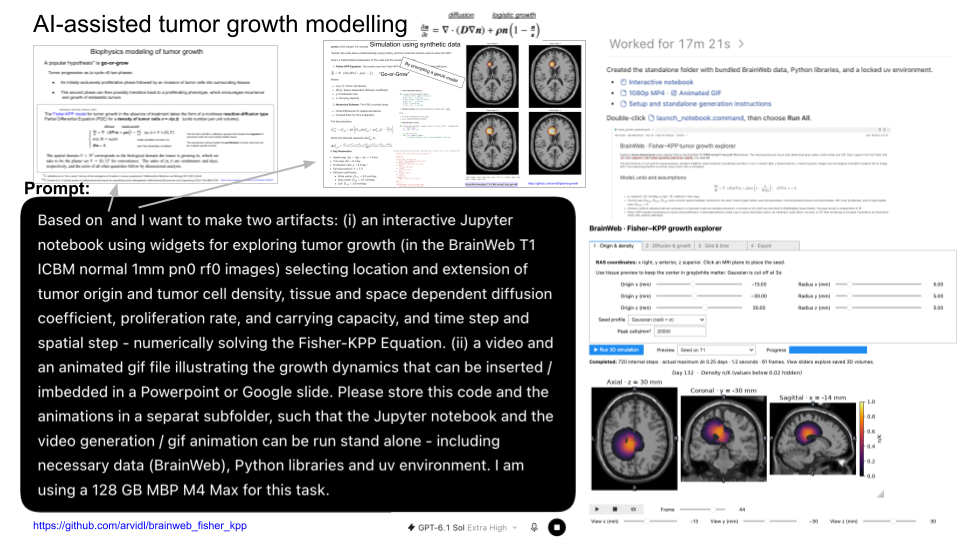
\includegraphics[width=.64\linewidth]{figures/talk/slide-18.png}}
\biopath
The prompt asks AI to build an interactive growth model in a BrainWeb anatomical image and to export an animation. The resulting interface makes assumptions manipulable: starting location, seed size, dispersal, proliferation and time can be varied. This is useful for learning because a predicted consequence can be compared with a simulated result. However, the normal BrainWeb brain is an anatomical phantom. The tumour field is generated by the model; it is not a tumour observed in that brain.

Use \coursenotebook{14b_brainweb_growth.ipynb}{Notebook 14b} for the self-contained course version. Before running, predict which tissue regions the chosen coefficients will make easier to traverse. Then change one assumption and compare matched times and display settings. Ask separately how the density changes and how a visible outline changes. A larger coloured region could reflect greater density, a lower threshold or a more permissive display. A more realistic-looking background does not turn assumed dynamics into patient-specific evidence. Record the anatomical source, model parameters and displayed quantity when sharing an animation. This preserves its value as an experiment on a mathematical model while making clear what additional observations would be needed to study an actual patient's progression.
\comppath
The prompt mixes scientific specification, software engineering and media production. Decompose it into a solver with testable inputs and outputs, an interface that changes parameters, and a renderer that reads saved states. The solver should work without the widgets. Cached states should allow slice, threshold and time controls to update displays without silently rerunning a different simulation. Exported animations should record the same parameter settings and states shown interactively.

The local BrainWeb lesson uses a density fraction $u=c/K$ and tissue-dependent scalar diffusivity. Scalar white/grey matter differences do not implement directional diffusion along fibre tracts. Physical voxel spacing and orientation must enter the calculation; coarser sampling can remove narrow barriers. Explicit time steps also need a stability bound that reflects grid spacing and diffusion. The course interface rejects unstable requested steps and distinguishes pending parameter changes from displayed cached states. Inspect these behaviours before interpreting an animation. As an exercise, keep the physical seed definition fixed while changing the grid, then compare integrated density and spatial spread. Explain which discrepancies plausibly arise from discretisation and which arise because the sampled anatomy itself has changed. This is more informative than checking whether both movies look smooth.
\end{slidenotes}

\begin{slidenotes}{19}{From a biological diagram to coupled variables}{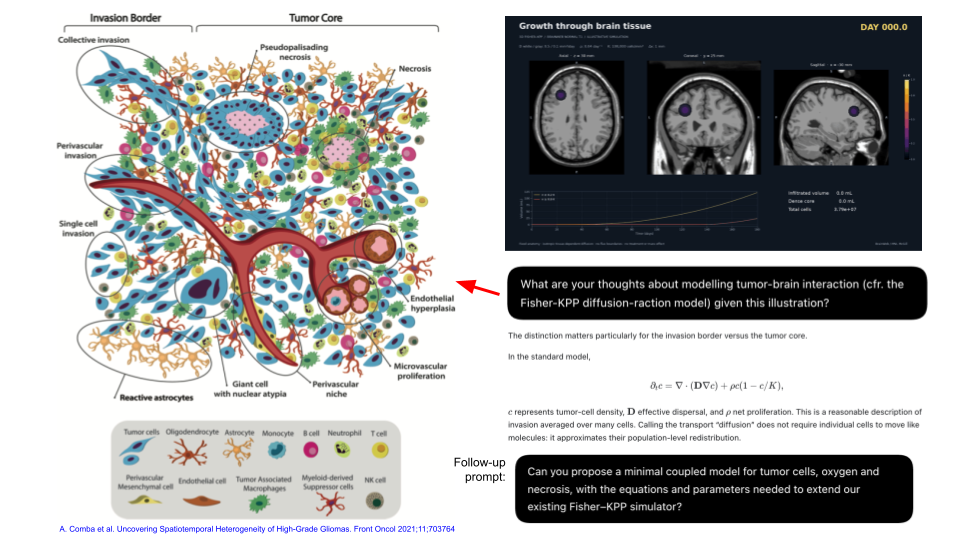
\includegraphics[width=.64\linewidth]{figures/talk/slide-19.png}}
\biopath
The histological schematic contrasts an invasion border with a heterogeneous tumour core. It depicts vessels, immune and stromal components, necrosis and different invasion patterns. Its role is to show how much biology is compressed when a model uses a single density field. The follow-up prompt asks for a minimal extension involving viable tumour, oxygen and necrotic material. That is a modelling proposal inspired by the diagram, rather than a derivation uniquely determined by it.

To interpret the proposal, tell a causal story in plain language. Oxygen can be supplied and consumed; low availability can affect survival; dead tissue can accumulate or be removed. Then ask which parts of that story the chosen equations actually represent and which remain assumptions. A dark region in an oxygen panel is a model state, not automatically a measured hypoxic region or an MRI compartment. The same caution applies to simulated necrotic material. Compare the extended model with the simpler Fisher--KPP reference under matched starting conditions. If the patterns differ, identify which added relationship caused the difference. A richer diagram can motivate a richer model, but additional biological vocabulary increases the need for clear definitions and discriminating observations.
\comppath
Begin with a state vector such as viable density, oxygen availability and necrotic material. Define the units and domain of each component before proposing coupling terms. Oxygen consumption should appear in its own balance; conversion from viable to necrotic material needs compatible units and signs. A production term for one compartment may require a corresponding loss from another, depending on the stated conservation assumptions. Normalised oxygen availability is not a concentration unless a scale has been defined.

The external implementation linked in the presentation guide supplies one illustrative closure: specific mathematical choices that complete the biological sketch. Those choices are unvalidated assumptions, not a unique model implied by the image. Test non-negativity, boundary behaviour and limiting cases, including whether disabling the added effects recovers the intended simpler dynamics. Identify parameters that the available observations could not determine separately. Increasing the number of adjustable coefficients can improve fit while making the mechanism less identifiable. For an exercise, propose two different oxygen-consumption rules that produce similar tumour outlines. Name an additional measurement that might distinguish them. The exercise shows why agreement with a single visible boundary offers limited evidence about the hidden processes represented in a coupled model.
\end{slidenotes}

\begin{slidenotes}{20}{Compare states with matched displays}{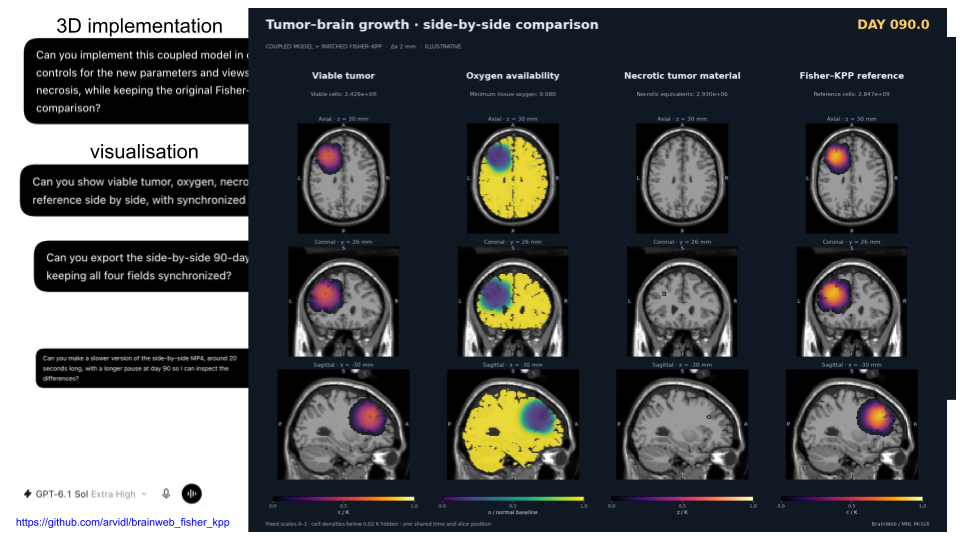
\includegraphics[width=.64\linewidth]{figures/talk/slide-20.png}}
\biopath
The four columns show simulated viable tumour, oxygen availability, necrotic material and a Fisher--KPP reference at a matched time and slice position. The comparison is useful because it separates quantities that a single coloured overlay could conflate. Read the colour bars before interpreting the images. A density fraction and normalised oxygen availability may both range from zero to one while referring to different states. A similar colour therefore does not imply a similar biological amount.

The anatomical background supports spatial orientation, while the overlays show outputs of an illustrative simulation. The extra oxygen and necrosis components have not thereby become measured patient properties. For a fair visual comparison, keep time, physical plane, colour scale and threshold conventions fixed. An apparent difference can otherwise be created by a changed display. Look for both local effects and changes in an integrated quantity. In particular, a thresholded volume asks how much tissue lies above a chosen value; integrated density asks how much modelled burden is distributed over the domain. Explain a case in which those quantities move differently. This develops the ability to read a simulation figure critically rather than equating a visually plausible animation with evidence that its mechanisms describe disease.
\comppath
Synchronisation is an experimental constraint. Store a common time index and physical slice coordinates for all fields, and compare the coupled model with a reference using documented initial conditions, grid and parameters. Fixed colour limits make changes over time interpretable; autoscaling can make a weak field look as intense as a strong one. State any masking or transparency threshold, because hidden low-density values still contribute to some numerical summaries.

For the local three-dimensional lesson, integrated density fraction is $B=v\sum_i u_i/1000$ in mL when each voxel has volume $v$ in mm$^3$. A thresholded volume is $V_\tau=v\sum_i\mathbf{1}[u_i\geq\tau]/1000$. The former is a volume-weighted model burden, and the latter is the volume of a thresholded set. Neither is an absolute cell count without the carrying-capacity scale. These definitions should accompany a numerical comparison even when the video supplies its own labels. Validate the renderer by checking that a stored voxel value agrees with its plotted position and colour. Validate the solver separately through numerical checks. The side-by-side view tests the consequences of modelling choices; it does not by itself establish which choice is biologically correct.
\end{slidenotes}

\begin{slidenotes}{21}{Agents produce different kinds of evidence}{
\includegraphics[width=.64\linewidth]{figures/talk/slide-21.png}}
\biopath
The PrimeView introduces agentic systems as workflows that coordinate reasoning and actions \citep{primeview2026}. The four output categories on the slide form a useful evidence ladder. Extracted information can support a literature map. Ranked hypotheses can guide a study. Iteratively refined candidates can focus resources. Empirically validated knowledge requires observations that test a claim. Producing an articulate hypothesis or an improved candidate does not skip those evidential steps.

Imagine an agent suggesting that an oxygen-sensitive growth model explains an imaging pattern. First check whether the cited studies support the extracted statements. Next examine whether the proposed hypothesis is distinguishable from alternatives. Then decide which observation could test it and whether the study design measures that observation adequately. A fluent chain connecting these stages can conceal a weak link. Natural-language or voice interaction can make the workflow easier to use, but the interface does not supply validation. Preserve the sources, intermediate decisions and failed tests that allow another investigator to examine the chain. The practical learning goal is to classify an output correctly and identify the next justified step. This makes AI assistance valuable without confusing the production of research material with the establishment of a scientific result.
\comppath
An agentic workflow can include a language model, tools, memory, branching logic and stopping criteria. The unit to reproduce is the resulting procedure, including tool versions and permissions, rather than a prompt alone. Save inputs, retrieved sources, tool arguments, outputs and decisions in a trace. A later reader should be able to identify where a claim entered the workflow and whether it was checked against an external observation.

Repeated runs under the same setup probe stochastic variability or technical repeatability. They are not independent biological replicates. Distinguish a rerun on the same data, a new sample from the same study and an independent study with its own acquisition and analysis. Those repetitions address different uncertainties. Also report unsuccessful runs where they affect the claimed reliability; selecting the best of many trajectories changes the meaning of the result. For an exercise, design an agent that proposes growth parameters from generated observations. Specify which actions it may take, which data it may inspect and when it must stop. Keep a forecast time point unavailable during fitting. The ability to inspect a complete trace then supports an audit of both procedural correctness and whether the final evaluation remained independent.
\end{slidenotes}

\begin{slidenotes}{22}{Place assistance inside the research design}{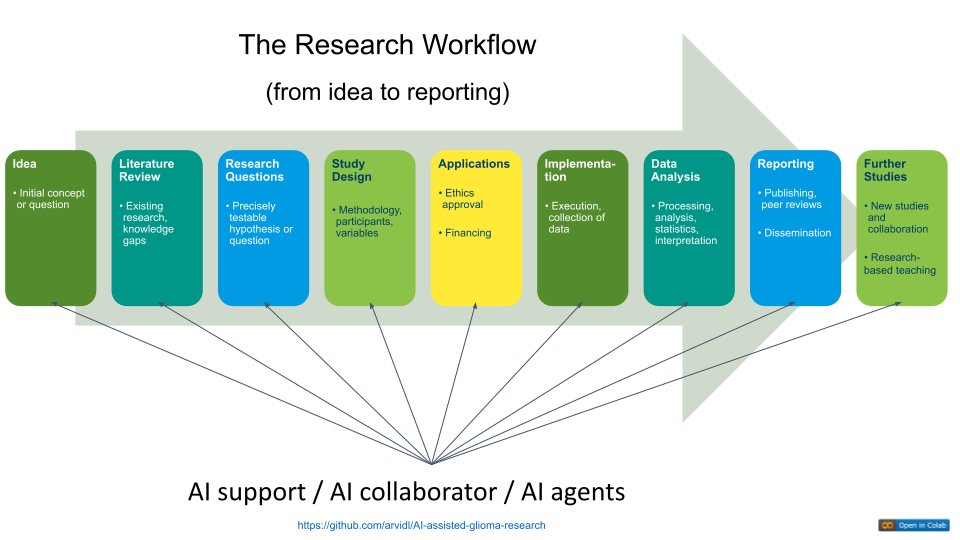
\includegraphics[width=.64\linewidth]{figures/talk/slide-22.png}}
\biopath
The workflow runs from an idea through literature review, a precise question, design, approvals and funding, implementation, analysis, reporting and further studies. AI support can enter at each stage, but each stage has its own criterion for success. A plausible research question must become answerable; an analysis must match the design; a report must preserve what was actually done. Ethics approval and appropriate data access belong to the study's conduct and cannot be inferred from a working analysis script.

Follow one example through the boxes: can serial imaging constrain a tumour-growth model sufficiently to forecast a later observation? Define which imaging quantity is measured, how examinations are aligned, and which time point is withheld. Decide what forecast error would matter before inspecting the final observation. Consider alternatives such as persistence of the most recent measurement. A model can fit earlier images closely without forecasting well, and a successful forecast does not establish a treatment effect. Use AI to draft plans, inspect code or organise evidence, while assigning scientific decisions to identifiable investigators. The diagram's return to research-based teaching closes the loop: explain the assumptions and failures, not only the result that survived to the final figure.
\comppath
The workflow can be represented as dependencies among research artefacts: a question, protocol, dataset version, analysis code, results and report. Record those dependencies so that changing an input identifies which outputs need to be recomputed. Freeze the primary evaluation before looking at its results. Automating a pipeline is useful, but a faithfully automated analysis can still answer an inappropriate question or use leaked information.

\coursenotebook{14c_growth_parameter_recovery.ipynb}{Notebook 14c} makes this distinction concrete with generated observations. It fits a diffusion scale and proliferation rate using selected earlier times, while day 90 remains withheld. The generating model, observation operator and parameter grid are controlled; the true pair is included among the candidates. This demonstrates parameter recovery and a forecast under favourable, specified conditions. It does not establish patient-level identifiability or clinical forecasting accuracy. The reference and fitting calculations use different time steps, but share the model family and spatial grid, so the test does not probe every form of model discrepancy. Compare the withheld forecast with persistence and explain both errors. Then propose one mismatch---an uncertain seed, changed observation operator or altered tissue map---that would make the task more realistic. State what additional evidence would be needed to interpret that new experiment.
\end{slidenotes}

\begin{slidenotes}{23}{A creative workflow and its provenance}{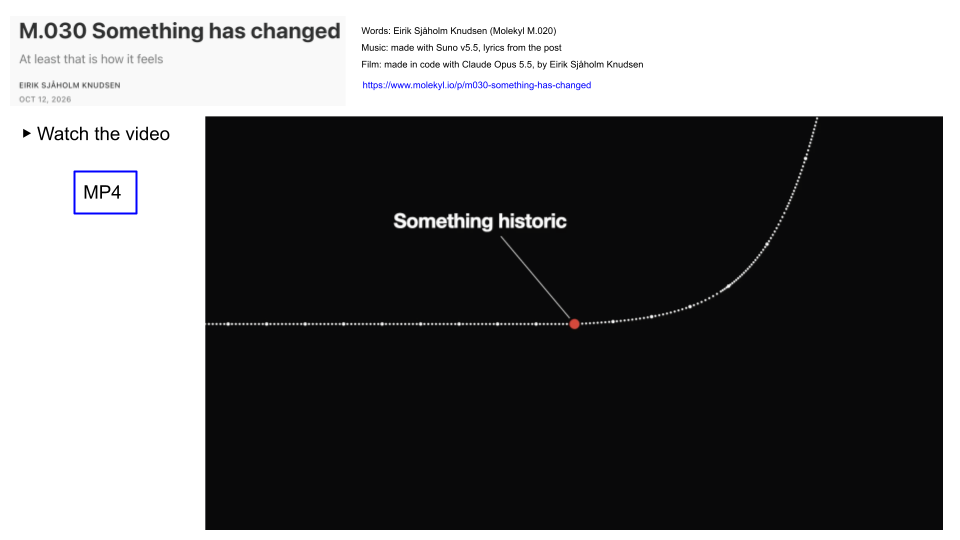
\includegraphics[width=.64\linewidth]{figures/talk/slide-23.png}}
\biopath
The slide introduces Eirik Sj\aa holm Knudsen's \emph{Something has changed}, a creative example combining human-written words, generated music and a film produced through code-assisted iteration. His accompanying post describes revisiting earlier writing in different media \citep{knudsen2026changed}. Use the example to examine collaboration and reception. A work can affect an audience through its words, rhythm, images and context even when parts of its production are automated. That response is evidence about the audience's encounter with the work, not a direct test of experience in the generating system.

The biomedical connection is communication. An animation or carefully chosen metaphor can make a difficult idea accessible, but emotional force can also make uncertain claims feel more settled than they are. If you use generated media to explain a model, distinguish the explanatory image from observed anatomy and state what the illustration simplifies. Ask viewers what they understood rather than assuming that attention implies understanding. In a short exercise, describe one concept twice: first as a factual paragraph, then as a proposed visual sequence. Identify which details the visual version leaves out and whether those omissions change the scientific meaning. The creative opportunity and the responsibility to preserve meaning belong together.
\comppath
Separate the stages of the media pipeline: source text, musical generation, visual specification, code, rendering and editing. Each has inputs and revision decisions. The model and tool names credited on the slide describe the reported production workflow; they do not provide a controlled comparison of those tools. Keep source material and generated artefacts distinguishable so that a later reader can identify which claims or creative decisions came from which stage.

For reproducibility, save the code and assets needed to render a chosen version, together with relevant settings and dependencies. Exact replay of a generation service may be unavailable even when deterministic rendering from saved assets is possible. These are different limits and should be documented separately. Evaluate a scientific animation by checking its correspondence to the underlying data or explanation, not only its visual quality. If the work suggests a dramatic reduction in labour, treat an AI-produced estimate of hypothetical human production time as an unvalidated estimate rather than a measured productivity study. Design a comparison with defined outputs and recorded effort if that claim matters. The example is strongest as an inspectable case of iterative creative collaboration, from which testable questions about quality, accessibility and effort can be developed.
\end{slidenotes}

\begin{slidenotes}{24}{Video interlude: observation and interpretation}{
\includegraphics[width=.64\linewidth]{figures/talk/slide-24.png}}
\biopath
The supplied static export contains a black panel with a red cross and a small credit to Knudsen and Molekyl. It does not contain a readable video frame. Treat this page as a companion to the preceding media example; motion, sound and additional content cannot be recovered from this PNG. The \href{https://www.molekyl.io/p/m030-something-has-changed}{creator's accompanying post} provides context for viewing the work separately. This distinction matters when an appendix must remain usable without the live presentation.

Use the interlude for a structured discussion. First describe something you actually observed in the work or its documented production. Next state your interpretation. Finally identify a claim that would require further evidence. For example, feeling that a sequence is compelling differs from establishing that it improves scientific understanding. If you have not watched it, keep the discussion about the documented workflow and avoid inventing its effects. In biomedical communication, the same discipline helps when a missing sequence, unavailable scan or incomplete record invites a plausible story. State the missing evidence, preserve what is known and specify what you would need to examine next. This is an exercise in careful interpretation as much as a discussion of creative technology.
\comppath
A presentation file, a static slide export and a rendered video preserve different information. A PNG can document layout and embedded credits while losing playback, timing, transitions or linked assets. The placeholder on this page illustrates what can be lost in a static export. It is not evidence that the original media lacked content or that a viewer saw the same panel during playback. Distinguish the source object from the particular export you can inspect.

For a computational exercise, specify a media manifest with the slide number, source asset, rendering method, duration where known, and a text alternative. Check that assets resolve and that the text alternative preserves the instructional purpose. If a video visualises simulated data, record the state files, time sampling, physical coordinates and colour mapping used to generate it. A static appendix can then link to the motion while retaining an explanation that stands alone. Evaluate accessibility and scientific faithfulness independently of whether playback succeeds. Apply the same principle to notebook outputs: a saved figure is evidence of a rendered result, whereas rerunning the computation additionally tests whether the documented environment and inputs reproduce it. The missing frame becomes a useful lesson in what a reproducible artefact must preserve.
\end{slidenotes}

\begin{slidenotes}{25}{Synthesis and a next experiment}{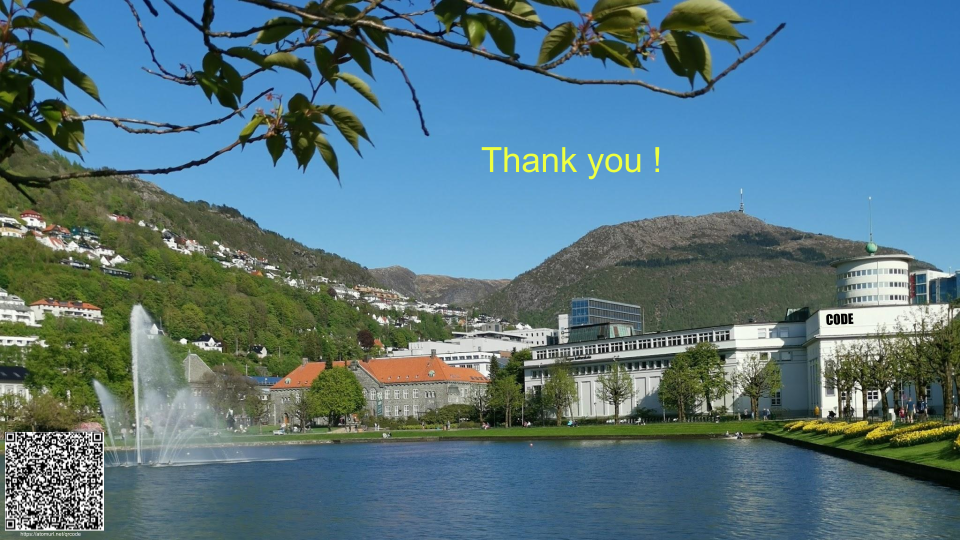
\includegraphics[width=.64\linewidth]{figures/talk/slide-25.png}}
\biopath
The closing image is an invitation to return from the presentation to a question in your own work. Select one model claim and explain it using the distinctions developed across the slides. What was measured? What was represented? Which process was assumed? What would a person do with the result? A useful synthesis connects these questions rather than concluding that machines are either wholly equivalent to people or irrelevant to human understanding.

For a concrete final exercise, interpret a positive test before recommending an action. With 1\% prevalence and both sensitivity and specificity at 90\%, a hypothetical group of 10,000 contains 90 true positives and 990 false positives. Thus only about 8.3\% of positive results are true positives. This expected-count example is constructed, not a measured diagnostic study. The appropriate action also depends on consequences and further evidence. \coursenotebook{15_ppv_and_decisions.ipynb}{Notebook 15} develops the calculation. Explain it to a colleague without beginning with a formula, and ask the colleague to describe the result back to you. Finish by naming one observation that would change your conclusion. That final sentence turns a confident-looking answer into a claim whose limits another person can examine.
\comppath
Choose a small reproducible investigation and state its purpose, algorithm and implementation. The course offers several routes: an input intervention in segmentation, a numerical limiting case, a threshold-versus-density comparison or a withheld growth forecast. Specify which output would count against your preferred explanation. Preserve the input, parameters, code version and result so that the test can be repeated. Report a failure with enough detail to make it useful for the next attempt.

For a final decision exercise, suppose $p$ is a calibrated event probability, a false positive costs one unit and a false negative costs four, with zero cost assigned to correct decisions. Acting has expected loss $1-p$; not acting has loss $4p$. Acting is favoured when $p>0.2$, with a tie at the boundary. These stipulated losses illustrate a decision rule; they are not clinical recommendations. Distinguish this probability threshold from an operating threshold used to obtain a classifier's sensitivity and specificity. The calculation links prediction to action only through its explicit assumptions. End your investigation with the same discipline: state the measured result, the assumptions needed for its interpretation, and the additional test required before extending the claim to a new population, mechanism or use.
\end{slidenotes}
\endgroup

\FloatBarrier
\clearpage
\begingroup
\small
\setlength{\bibsep}{3pt}
\interlinepenalty=10000
\bibliographystyle{plainnat}
\bibliography{references}
\endgroup
\end{document}
